\chapter{Mobiliser des outils de \textit{computer vision} pour relever les imitations et ré-interprétations techniques et iconographiques}
\markboth{}{}

\epigraph{\og In Andean textiles, there is a deep harmony between image and structure.\fg}{William J. Conklin, 1997, \og Structure as Meaning in Andean Textiles. \fg, p.~118.}


\section{Analyse des sources iconographiques}
\subsection{Les images : sources de savoir sur les influences iconographiques ?}

Les données géographiques de la base de données nous ont permis de détecter certains foyers de production textile ainsi que certaines circulations physiques des pièces.  Des circulations textiles ont certes lieu mais, comme nous l'avons vu dans le premier chapitre du mémoire, une partie des évolutions des tissus se fait par imitations ou ré-interprétations iconographiques et techniques. Ces modifications sont détectables en analysant directement les objets et le recours à des outils de \textit{computer vision} semblent adéquats pour les saisir. Nous entendons par \textit{computer vision}, le domaine de l'intelligence artificielle qui, à partir d'images numériques, obtient des informations significatives.

Certaines sociétés se sont influencées à travers les conquêtes mais aussi par les échanges ou la proximité géographique. 
Ainsi, les sociétés voisines Chimú et Chancay, sur la côte centrale du Pérou, partagent des traits culturels communs. Dans la base de données, nous pouvons observer cela à partir de poupées utilisées dans les sépultures. Elles représentent la même divinité homme-ours. Leurs visages sont réalisés en tricot dont partent des cordons et une frange qui forment le corps et les cheveux. Les traits du visage sont formés par quelques points simples de broderie (passé-plat ou chaînette). Ce cas nous montre la complexité de la compréhension des influences entre civilisations, puisqu'il s'agit de civilisations voisines en conflit mais qui ont probablement eu des échanges et dont on sait qu'elles partageaient certaines pratiques rituelles et croyances. Saisir les influences permet donc d'aller au-delà des changements iconographiques et techniques et de saisir l'évolution de traits culturels fondamentaux dans les sociétés, comme les pratiques rituelles d'inhumation. 


\begin{figure}[!h]
    \begin{minipage}[c]{.5\linewidth}
            \begin{center}
                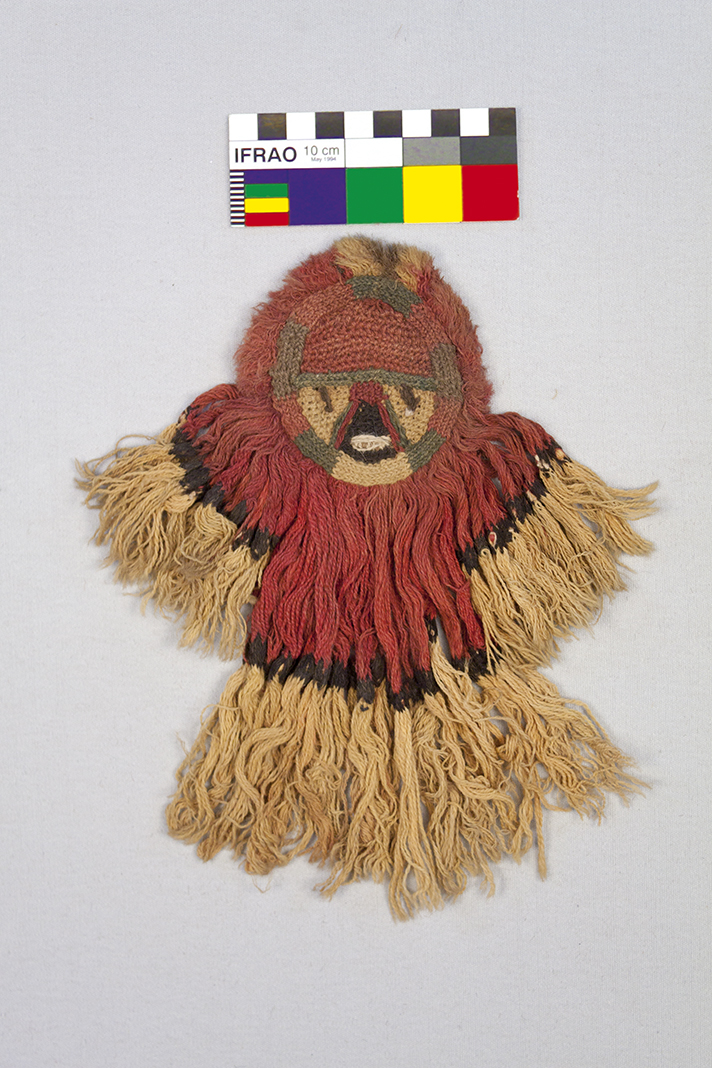
\includegraphics[width=5cm]{../images/BML059.jpg}
            \end{center}
    \end{minipage}
        \begin{minipage}[c]{.5\linewidth}
        \begin{center}
        		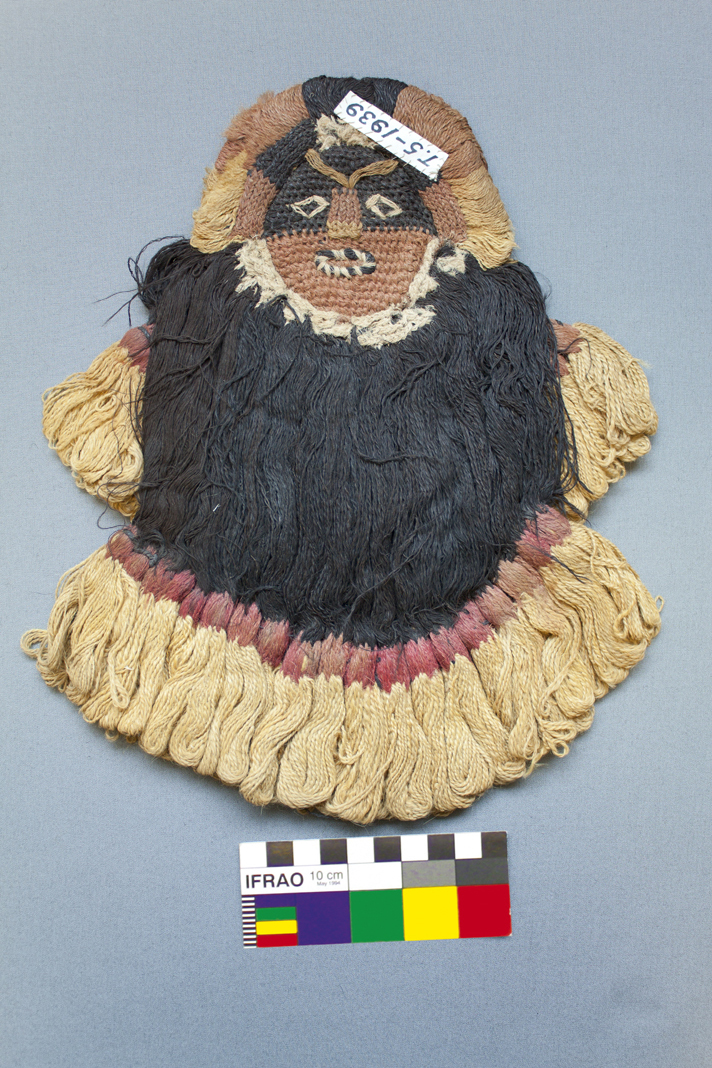
\includegraphics[width=5cm]{../images/VAM018.jpg}
	\end{center}
    \end{minipage}
   \caption{Poupées d'enterrement Chancay et Chimú tardif. \\ Références dans la base de données : BML059 et VAM018.}
   \label{fig:poupees}
\end{figure}


Comme nous l'avons vu, à l'Horizon Récent, les cultures s'influencent avec la culture Inca qui s'impose sur tout le territoire tout en gardant les spécificités locales des populations\footcite[p.~53]{nilesArtistEmpireInca1994}.
Le textile ci-dessous mélange ainsi le style inca, par les couleurs, la forme du sac, la technique à dominante chaîne et les finitions des bordures, avec le style Chimú sur la lanière en double-étoffe qui contient des personnages anthropomorphiques typiques de cette civilisation.
\begin{figure}[!h]
	\begin{center}
		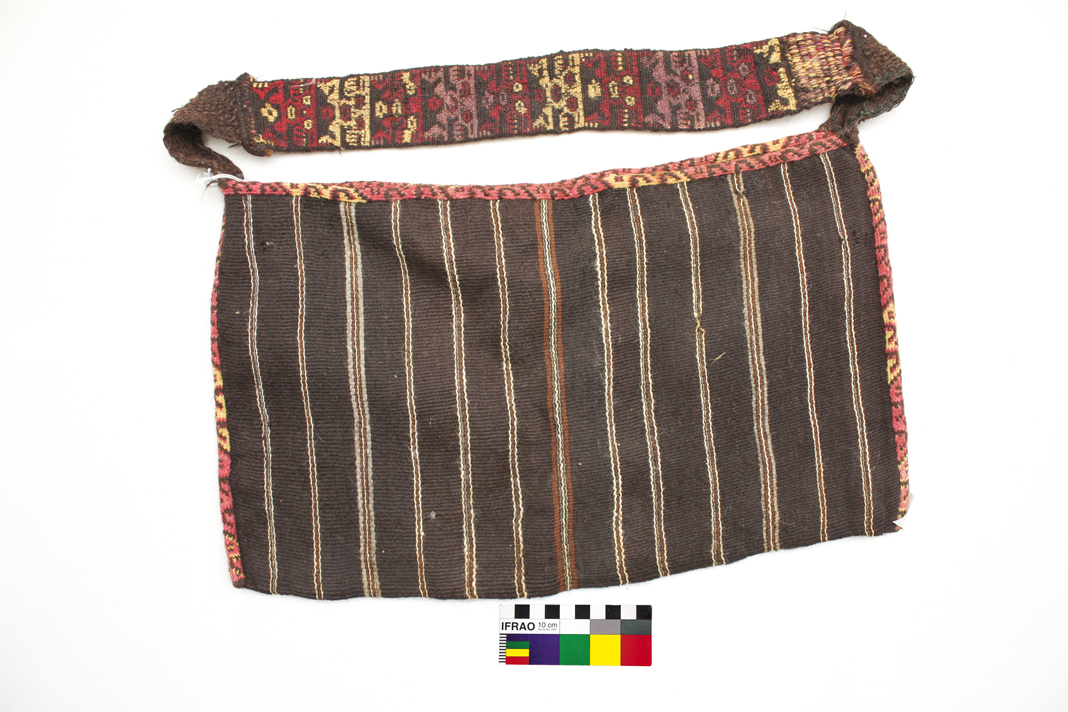
\includegraphics[width=10cm]{../images/MSF066.jpg}
		\caption{Exemple de textile métissé entre Chimú et Inca. \\ Référence dans la base de données : MSF066}
		\label{fig:MSF066}
	 \end{center}
\end{figure}

Ces deux cas nous amènent à réfléchir selon deux axes. Comme le soulignent Sven Helmer et Vuong M. Ngo dans leur proposition de mesure de similarité entre les textiles, comprendre la structure interne des textiles \og peut aider les experts du domaine à mieux comprendre comment les textiles ont évolué au fil du temps et se sont diffusés dans différentes régions\footnote{\cite[p.~163]{helmerSimilarityMeasureWeaving2018}. Citation originale : \textquotedblleft \textit{can help domain experts gain deeper insights into how textiles evolved over time and spread across different regions}\textquotedblright}.\fg \:Classifier les techniques à partir d'images permettrait donc de détecter si certaines sociétés partagent les mêmes traits techniques, indicateurs d'échanges ou d'influence. C'est un travail d'autant plus important qu'avec la numérisation des collections muséales les chercheurs et chercheuses travaillent de plus en plus à partir d'images d'artefacts. Par ailleurs, nous devons nous questionner sur les textiles détenant des traits iconographiques communs ou hybrides. Ce deuxième axe est d'autant plus adéquat que certains motifs sont propices à l'imitation car facilement transférables d'une technique à une autre, comme le relève Sophie Desrosiers pour les motifs \og en escalier qui peuvent être traduits en flottés de chaîne ou de trame\fg \footnote{\cite[p.~7]{desrosiersRevisitingOcucajeOpened2008} Citation originale : \textquotedblleft \textit{with stepped outlines which can be translated into warp or weft floats}\textquotedblright}. Dans les textiles andins, les motifs peuvent en effet difficilement être pensés hors des techniques puisque celles-ci contraignent la réalisation iconographique\footcite[p.~118]{conklinStructureMeaningAndean1997}. Dans le cas des textiles à dominante chaîne, l'organisation des fils, qui constitueront les motifs, doit être pensée en amont du montage sur le métier à tisser, illustrant l'imbrication entre techniques et iconographie. Ces motifs contraints sont donc possiblement détectables à partir du corpus d'images.

\subsection{Les sources iconographiques de la base de données \textit{Weaving Communities of Practice}}

La base de données \textit{Weaving Communities of Practices} est composée d'un corpus iconographique qui regroupe trois types d'images : des photographies, des croquis et des relevés textiles réalisés par logiciel de dessin assisté par ordinateur (DAO) (dans le même esprit que le relevé \ref{fig:BML044_schema}). Nous disposons de 162 modélisations par DAO, réalisées par les ingénieurs du projet. Les 83 croquis, réalisés à la main, font partie des collections du \textit{British Museum}.

\begin{figure}[!h]
    \begin{minipage}[c]{.4\linewidth}
            \begin{center}
                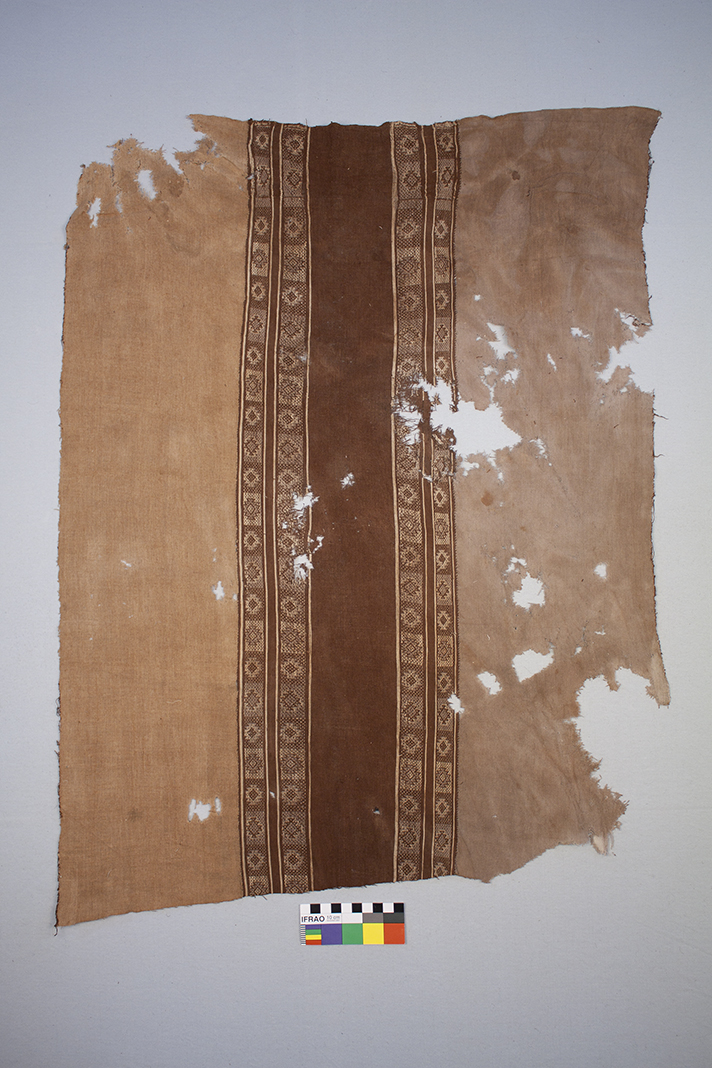
\includegraphics[height=6cm]{../images/BML026_IMG.jpg}
            \end{center}
    \end{minipage}
\hspace{5pt}
        \begin{minipage}[c]{.2\linewidth}
        \begin{center}
        		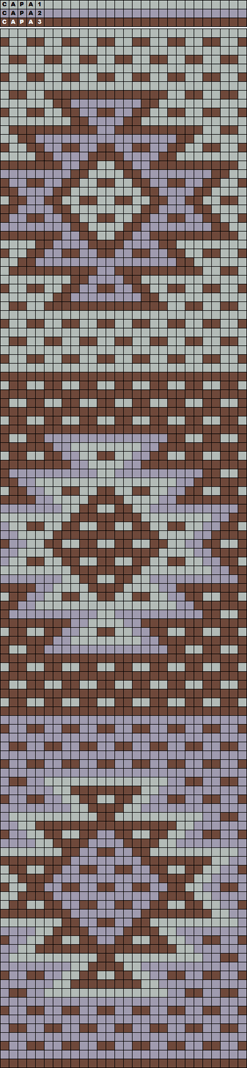
\includegraphics[height=6cm]{../images/BML026_Schema.png}
	\end{center}
    \end{minipage}
            \begin{minipage}[c]{.4\linewidth}
        \begin{center}
        		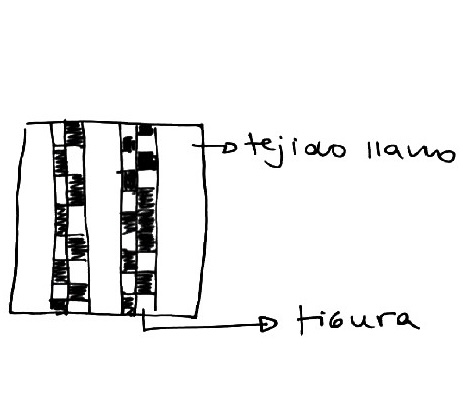
\includegraphics[height=6cm]{../images/BML026_croquis.jpg}
	\end{center}
    \end{minipage}
    \caption{Photographie, schéma et croquis pour un même textile. \\ Référence dans la base de données : BML026.}
\end{figure}

\noindent Le corpus d'images à partir duquel nous allons travailler ne contient ni les schémas ni les croquis, mais uniquement les photographies, soit 3301 images. Nous pouvons observer sur le schéma suivant le nombre d'images disponibles par textile et la répartition statistique de ce nombre sous forme de boîte à moustache. Les photographies sont toutes en couleur (3 canaux), elles contiennent soit les textiles entiers soit des détails de celui-ci ainsi que des supports (en bois, en carton) ou des personnes les portant, notamment dans les collections du musée national archéologique de Bolivie. 

\begin{figure}[!h]
	\begin{center}
		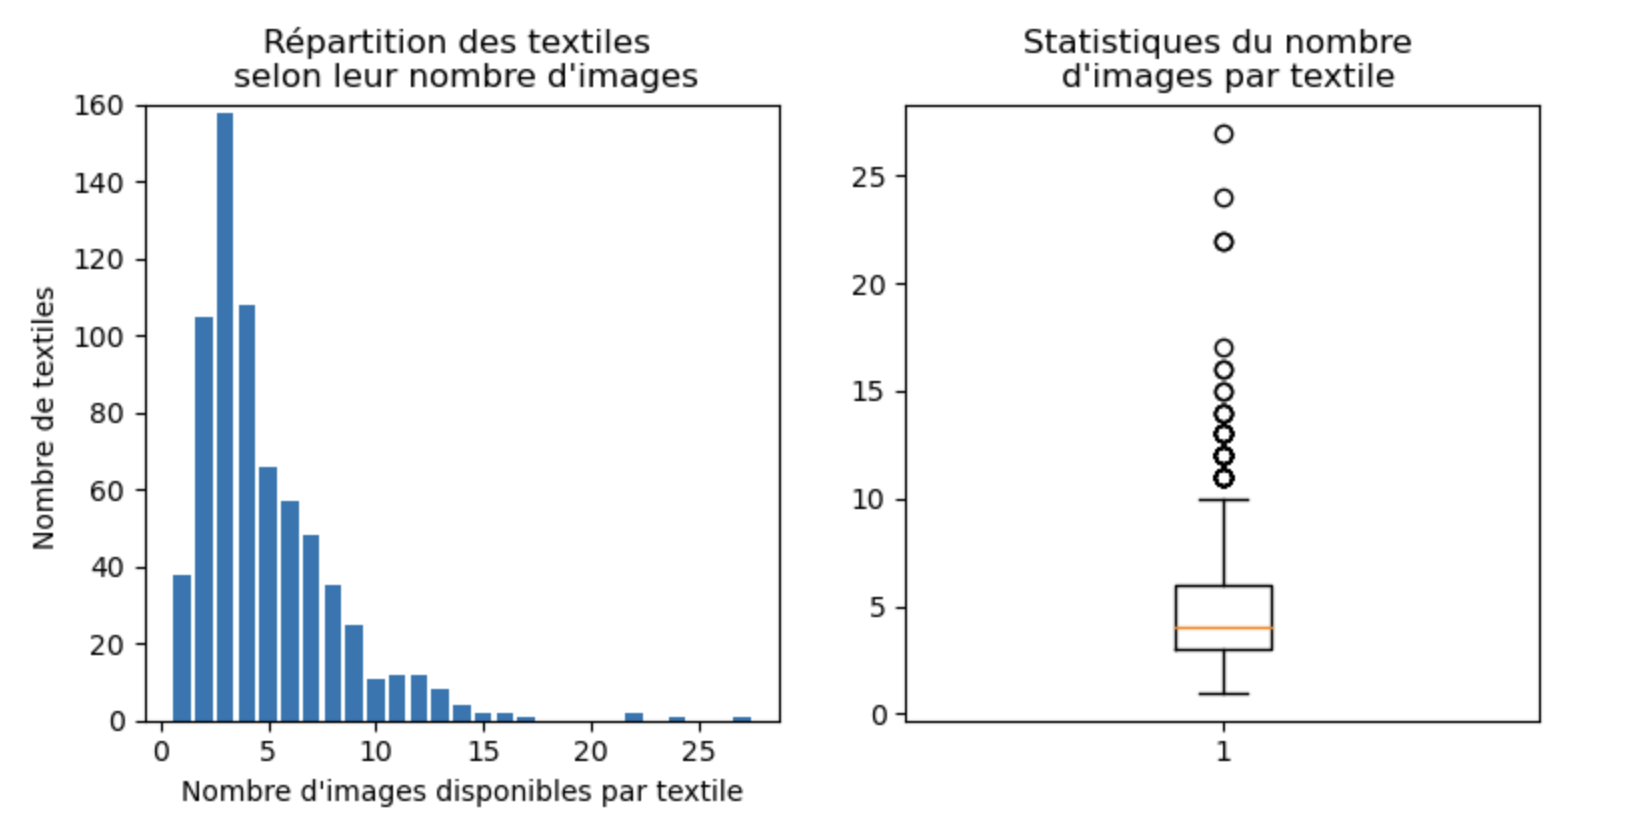
\includegraphics[width=16cm]{../images/nbImages.png}
	 \end{center}
	 \caption{Répartition des images par objet}
\end{figure}

\begin{wrapfigure}{r}{0.3\textwidth}
    \centering
    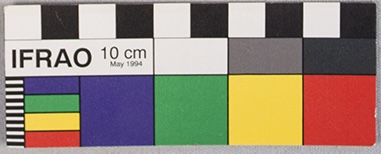
\includegraphics[width=0.3\textwidth]{../images/IFRAO.jpg}
    \caption{Règle IFRAO}
    \label{fig:IFRAO}
\end{wrapfigure}



Une grande partie des photographies contiennent une échelle IFRAO, réglette de 10 centimètres composée de carrés noirs, blancs et colorés (vert, rouge, jaune et bleu). Parue en 1994, cette échelle permettait initialement aux archéologues de calibrer les couleurs des \oe{}uvres d'art préhistoriques\footcite[p.~225]{lopezIFRAOStandardScale2009}. Les couleurs de la règle étant fixées numériquement, elles peuvent servir de référence pour le reste de l'image et ainsi ajuster les couleurs des artefacts au sein des images numériques. La présence de cette règle nous permet d'avoir une idée précise de la taille des pièces textiles et nous confirme la disparité de ces dernières : certaines mesurent plus d'un mètre de longueur et/ou de largeur et d'autres seulement un demi centimètre. Les images ont des dimensions analogues, la plupart ont leur largeur ou leur hauteur entre 700 et 800 pixels, et l'autre côté à 1068 pixels (voir schéma suivant).

Les images de la base de données ont presque toute la même résolution (nombre de pixels contenus dans un pouce (\textit{inch}) ou pixels par pouce). La résolution des images de la base de données est plutôt faible puisqu'on considère que la résolution d'une image est bonne autour de 250~ppp. Nous n'utiliserons donc pas ce paramètre dans la suite du traitement.

\begin{table}[!h]
    \centering
    \begin{tabular}{|c|c|}
        \hline
         \cellcolor{blue!20}\textbf{Résolution (\textit{dot per inch})} & \cellcolor{blue!20}\textbf{Nombre d'images} \\ \hline \hline
         72 &  3220 \\ \hline
         96 & 2 \\ \hline
         240 & 55 \\ \hline
    \end{tabular}
    \caption{Résolution des images de la base de données.}
    \label{tab:resolution}
\end{table}

\clearpage

\begin{figure}[!h]
	\begin{center}
		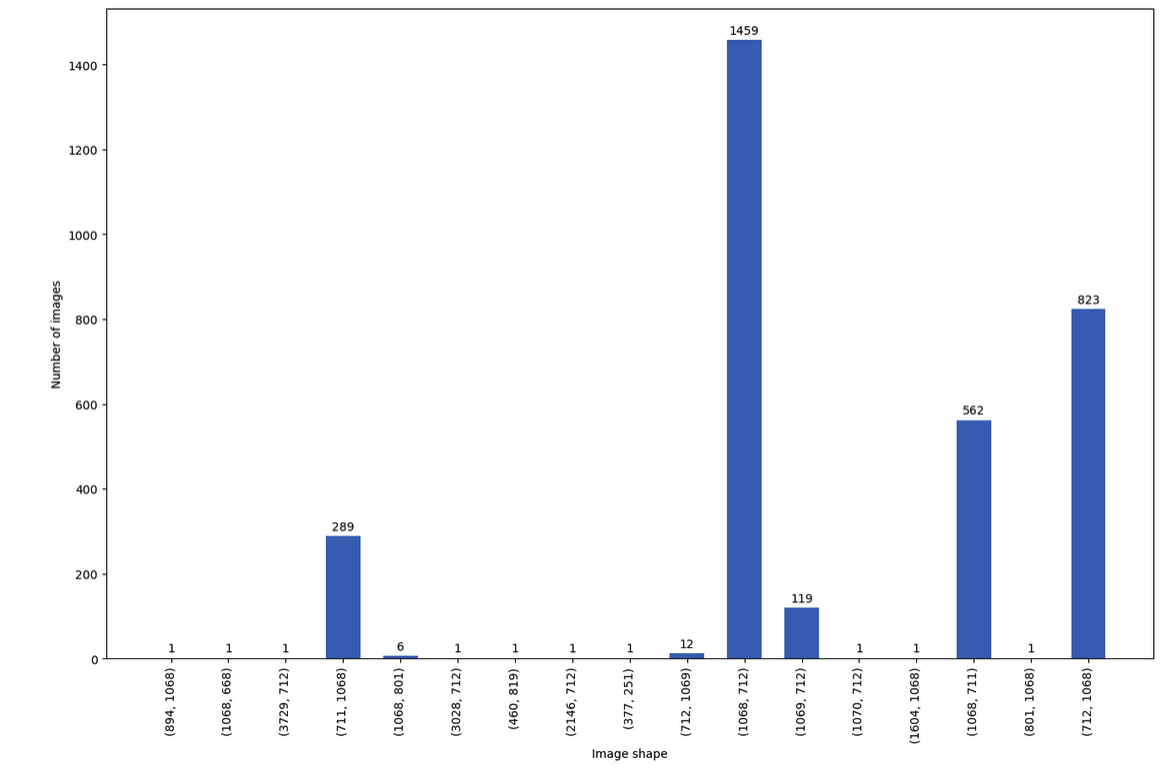
\includegraphics[width=16cm]{../images/dimension.png}
	 \end{center}
	 \caption{Répartition de la dimension des images}
\end{figure}


\section{Une classification automatique des techniques ?}

\subsection{L'apprentissage machine au service de la détection des armures textiles}

Un des indicateurs des influences entre sociétés porte sur les techniques utilisées par ces civilisations. Dans la plupart des cas, les techniques sont détectables à partir des armures, c'est-à-dire de la manière dont les fils sont entremêlés. La question des techniques est centrale en analyse des textiles et l'utilisation de l'apprentissage machine pour détecter des informations techniques à partir d'images est essentielle.


Comme le soulignent  Helmer et Ngo, la variété des armures textiles complexifie leur modélisation\footcite[p.~160]{helmerSimilarityMeasureWeaving2018}. C'est d'ailleurs une des limites aux propositions contemporaines de classification des armures textiles reposant sur l'apprentissage machine. Souvent destinées à une finalité industrielle, elles s'entraînent sur des armures simples au sein desquelles la trame et la chaîne sont visibles (toile, sergé et satin)\footcite[p.~6365-6369]{mengAutomaticRecognitionWoven2022}. Pour les armures plus complexes, la détection des techniques est réalisée après un lourd processus d'annotation\footcite[p.~169]{helmerSimilarityMeasureWeaving2018}. Travailler sur les armures textiles à partir d'images pose en effet question puisqu'il s'agit de saisir une structure en trois dimensions à partir d'images en deux dimensions. Ainsi, \og le dessin d'une étoffe façonnée -- produit par le tissage -- résulte d'un entrelacement et n'est pas un dessin de surface, imprimé sur étoffe ou sur papier\fg\footcite[p.~67]{leclercqEntretienAvecJeanPaul2016}. Nous posons l'hypothèse que certains éléments apparaissant sur les faces des textiles sont discriminants pour déterminer les techniques, notamment les lisières, les directions des fils ou les zones de finition des textiles.


\begin{figure}[!h]
    \centering
    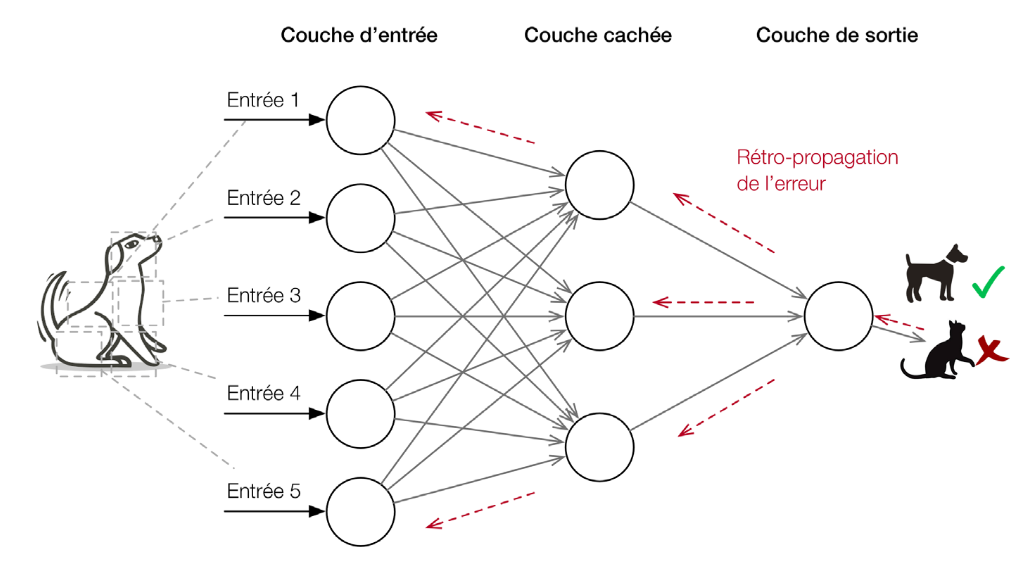
\includegraphics[width=12cm]{../images/resSimple_CardonP199.png}
    \caption[Structure simple d'un réseau de neurones]{Structure simple d'un réseau de neurones \\ Source : C\textsc{ardon} et al., 2018, p.~199}
    \label{resSimple}
\end{figure}

La classification automatique des textiles repose sur des méthodes d'apprentissage machine. Ce concept apparaît en 1943 quand Warren S. McCulloch et Walter Pitts proposent le premier modèle, dans le domaine de la neurophysiologie, qui est associé au concept d'apprentissage\footcite{mccullochLogicalCalculusIdeas1943}. C'est un modèle au sein duquel \og le neurone prend des variables en entrées, y applique un poids pour produire une somme qui, si elle dépasse un certain seuil, déclenche l'activation du neurone\footcite{cardonRevancheNeuronesInvention2018}\fg. Il faut attendre les années 2010 pour que ce type de modèle, \og réseau de neurones \fg, ainsi que ses développements dans les années 1980, soit réutilisé et adapté au traitement des images. Alex Krizhevsky, Ilya Sutskever et Geoffrey Hinton utilisent, en 2012, un réseau de neurones qui modifie profondément le domaine de la classification d'images\footcite{hintonImprovingNeuralNetworks2012}. Ils réussissent à classer un ensemble de plus d'un million d'images grâce à un réseau de neurones convolutif (CNN). Les CNN sont composés d'un ensemble de couches dont :
\begin{citer}
 	les couches additionnelles de neurones permettent d'apprendre des fonctions non linéaires. L'algorithme fonctionne en prenant la dérivée de la fonction de perte du réseau et en \textquotedblleft propage\textquotedblright \:l'erreur pour corriger les coefficients dans les couches basses du réseau\footcite[p.~198]{cardonRevancheNeuronesInvention2018}. 
 \end{citer}
 \noindent Dans notre cas, nous utiliserons le CNN \textit{You Only Look Once} (YOLO)\footcite[p.~1]{redmonYouOnlyLook2016}. Il alterne entre des couches de convolution (\textit{Conv. Layer}) au sein desquelles une fenêtre glissante parcourt l'image pour détecter les caractéristiques de l'images ou \textit{features}, et des couches de \textit{pooling} qui réduisent la taille de l'image d'entrée, en prenant la valeur maximum de la fenêtre considérée (\textit{MaxPooling})\footcite[p.~439]{lecunDeepLearning2015}. L'alternance entre ces couches permet de détecter les caractéristiques de chaque classe au niveau du détail (quand le nombre de pixels est élevé) et au niveau global (en réduisant le nombre de pixels). Ce modèle est notamment destiné à la classification d'objets, il divise l'image d'entrée en une grille de cellules, détecte les objets dans ces cellules et leur adjoint une classe. Dans notre cas, nous reprenons l'architecture de YOLO que l'on entraîne à partir de nos images et de nos classes. 
 \clearpage
 
 \begin{figure}[!h]
	\begin{center}
		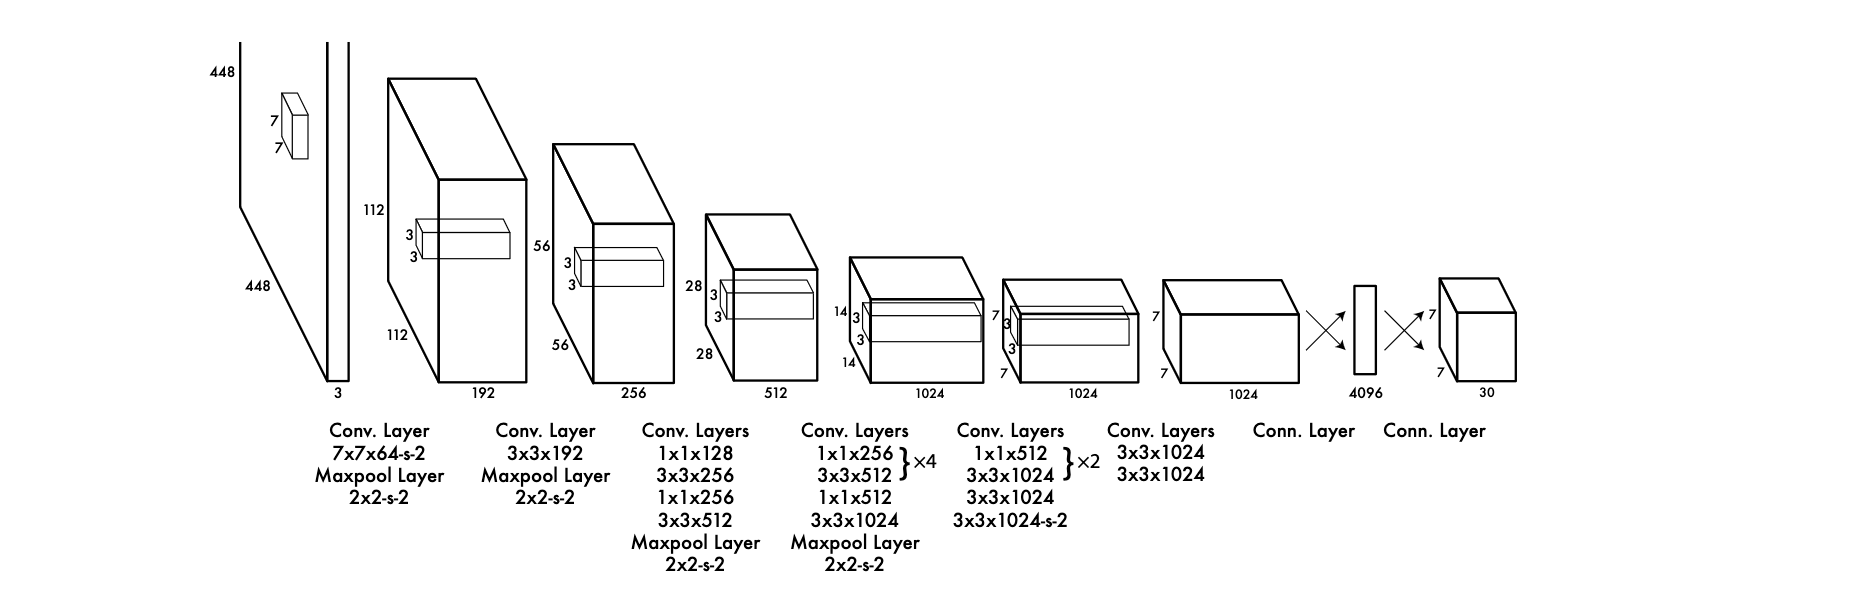
\includegraphics[width=18cm]{../images/YOLO_archi.png}
		\caption{Architecture du réseau YOLO. \\ Source : Redmond \textit{et al.}, 2016, p.~3.}
		\label{fig:YOLO}
	 \end{center}
\end{figure}


\noindent La classification a lieu en plusieurs étapes : 
\begin{itemize}
	\item Attribution de labels aux images ou annotation.
	\item Entraînement d'un algorithme à partir des données annotées.
	\item Récupération des poids obtenus lors de l'entraînement pour classifier les images.
\end{itemize}

\noindent L'annotation des images est réalisée à partir du vocabulaire interne de la base de données. Nous avons utilisé la catégorie \og fabric \fg \:(voir tableau \ref{fig:fabric}) que nous avons simplifiée en cinq classes : tissage dominante chaîne, tissage dominante trame, tissage mixte, maille/réseau et toile. La réduction du nombre de classes permet de rééquilibrer le nombre de cas par classe, critère important pour l'entraînement du modèle. Toutefois, ces classes portent uniquement sur le fond du textile, les ajouts comme les broderies, les franges, les pompons et les tresses cousus sur les tissus ne sont pas pris en compte.

\begin{wrapfigure}{r}{0.3\textwidth}
    \centering
    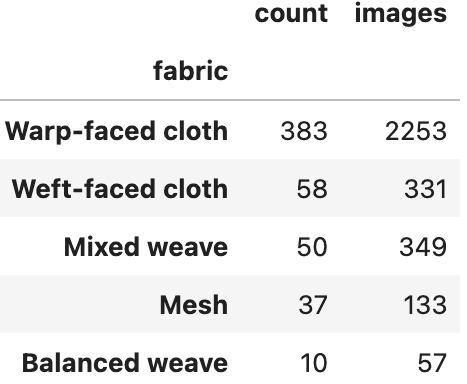
\includegraphics[width=5cm]{../images/fabricmodif.png}
    \caption{Classes modifiées.}
    \label{fig:classes_modif}
\end{wrapfigure}

Avant de décrire les différentes tentatives de classification, nous allons expliciter certains paramètres du modèle (en l'occurence, ceux que nous utilisons) : 
\begin{itemize}
	\item \textit{Epochs} : nombre de passages sur l'ensemble des données d'entraînement.
	\item \textit{Batch} : nombre d'images fournies avant que les paramètres internes du modèle ne soient mis à jour.
	\item \textit{Dropout} : taux de désactivation des neurones au cours d'une \textit{epoch} pour éviter le sur-apprentissage. Fixé à 0,1, il signifie que chaque neurone a une chance sur 10 d'être désactivé lors d'une \textit{epoch}.
	\item \textit{Seed} : graine aléatoire qui permet de reproduire les résultats (toutes configurations égales par ailleurs).
\end{itemize}

\subsection{La détection des armures textiles grâce à la classification supervisée des images}
Pour saisir la diffusion et l'hybridation des pratiques textiles entre civilisations, nous devons déterminer quelles sont les techniques utilisées, critère de similitude discriminant. Cette tâche a déjà été réalisée pour les soies européennes par l'équipe de SILKNOW, à partir d'un \textit{dataset} de 10 383 images\footcite[p.~51]{dorozynskiMultiTaskDeepLearning2019}. Leurs catégories sont moins précises que celles à partir desquelles nous travaillons puisque le tissage est regroupé en une catégorie. En revanche, ils prennent en compte les broderies et ajoutent le velours et le damas, techniques absentes de notre \textit{dataset}. N'étant pas en mesure de réutiliser leur code, nous avons développé une approche similaire de classification supervisée des images, utilisant un autre modèle d'apprentissage machine : YOLOv8\footnote{\url{https://docs.ultralytics.com/}, consulté le 27 avril 2024.}, dernière version du modèle YOLO.

\subsubsection{Classification à partir du \textit{dataset} initial.}
Nous avons réalisé une première tentative de classification à partir des images disponibles. Les cinq catégories sont partagées selon la répartition suivante :  
\begin{table}[!h]
    \centering
    \begin{tabular}{|c|c|c|c|}
        \hline
          \cellcolor{blue!20}\textbf{\textit{Fabric}} & \cellcolor{blue!20}\textbf{Technique} & \cellcolor{blue!20}\textbf{Nombre d'images}& \cellcolor{blue!20} \textbf{Pourcentage} \\ \hline \hline
         Warp-faced cloth & Tissage à dominante chaîne & 2051 & 72\% \\ \hline
         Weft-faced cloth & Tissage à dominante trame & 313 & 11\% \\ \hline
         Balanced weave & Toile & 54 & 2\% \\ \hline
         Mixed Weave & Tissage mixte & 315 &  11\% \\ \hline
         Mesh & Maille et réseaux & 127 &  4\%  \\ \hline
          & \textbf{Total} & \textbf{2860} &  \textbf{100\%}  \\ \hline
    \end{tabular}
    \caption{Répartition initiale des classes techniques.}
    \label{tab:classes_init}
\end{table}

Pour le premier entraînement tel quel, nous entraînons sur 2286 images réparties en 5 classes. 50 époques composent l'entraînement, avec des \textit{batchs} de 64 images et un \textit{dropout} de 0,1.

\vspace{4pt}
 
 \begin{minipage}{\dimexpr\textwidth-3cm}
	\textbf{Rappel sur les métriques permettant de juger des résultats du réseau de neurones}

	La fonction de perte (ou \textit{loss}) est un indicateur de l'optimisation du modèle au cours de l'entraînement, elle indique la différence entre le résultat attendu et le résultat prédit.
	
	La précision (\textit{accuracy}) permet de quantifier la qualité d'un modèle, elle calcule le nombre de classes qui ont été correctement attribuées aux images. Elle est intrinsèquement liée aux notions de Vrai Positif (VP) et Faux Positif (FP).
	\begin{itemize}
	    \item Vrai Positif : les classes correctement reconnues par le modèle. 
	    \item Faux Positif : les éléments qui sont reconnus comme appartenant à une classe alors qu'ils ne lui appartiennent pas 
	\end{itemize}

	La précision est ensuite calculée à partir du nombre d'éléments dans chaque catégorie selon l'équation suivante qui représente le recouvrement entre vérité terrain et prédiction : 

	\[ \frac{VP}{VP+FP} \] 
	
\noindent Au moment des prédictions, YOLO propose cinq classes possibles pour l'image. La \textit{top1\_accuracy} indique si la première classe proposée est bien la classe de l'image, la \textit{top5\_accuracy} indique si la classe de l'image se trouve dans les cinq premières classes proposées. Dans notre cas, ne disposant que de cinq classes, la \textit{top5\_accuracy} est toujours égale à 1.\\
 \end{minipage}

\begin{figure}[!h]
	\begin{center}
		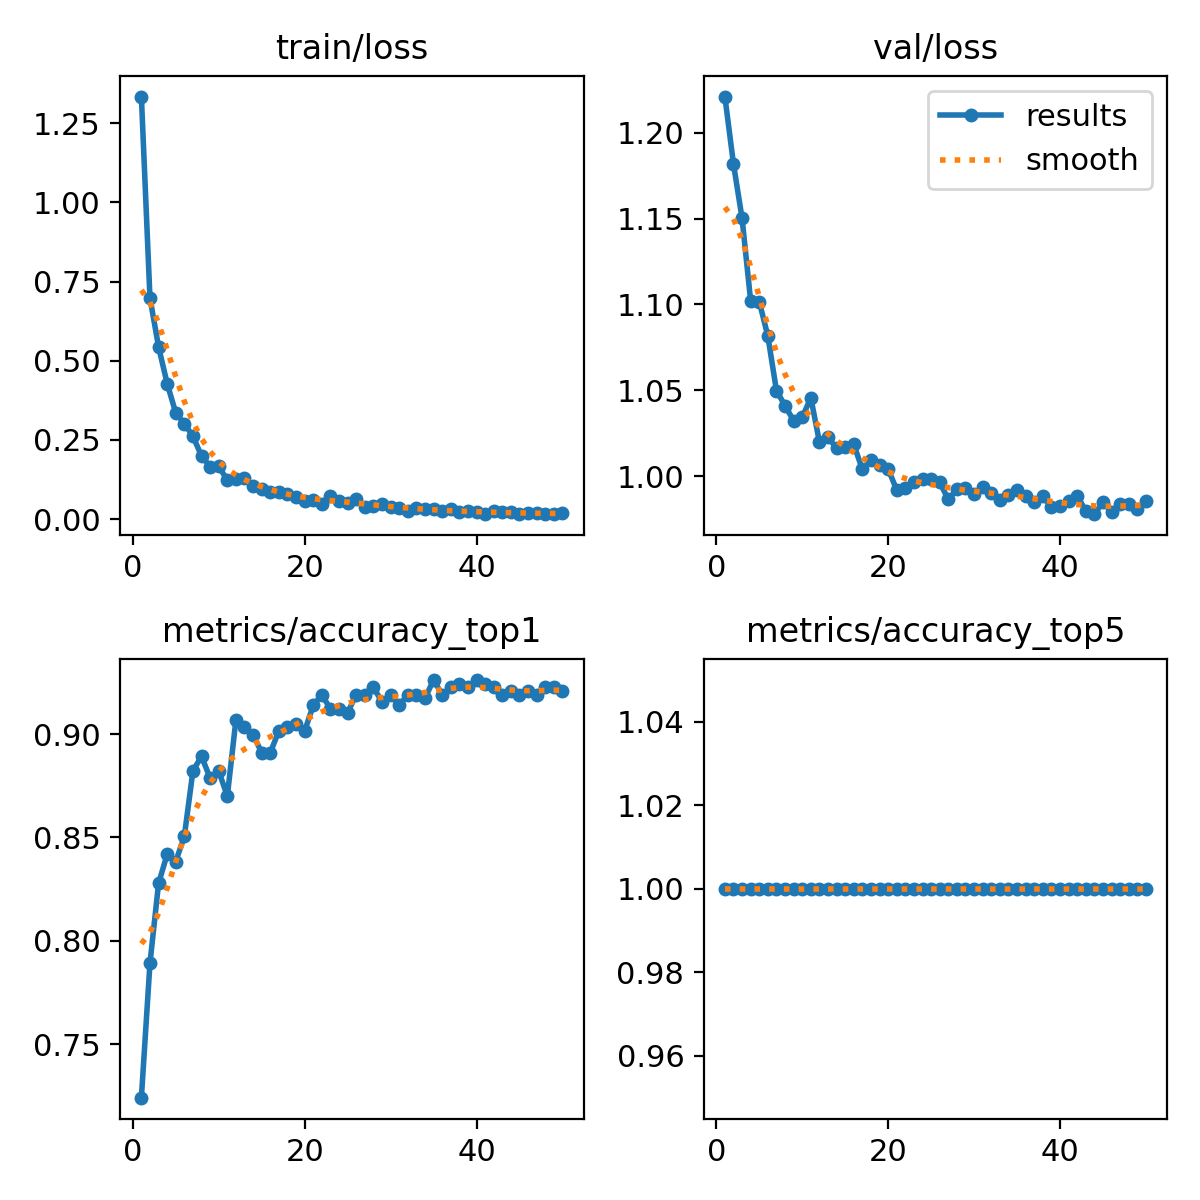
\includegraphics[width=12cm]{../images/YOLO_result50epoch.png}
		\caption{Résultats du premier entraînement YOLO sous forme de graphiques.}
	 \end{center}
\end{figure}

\noindent En observant les résultats de l'entraînement, nous pouvons voir qu'il atteint un palier autour de la $35^{eme}$ époque, avec un taux de précision atteignant 92\%.

Après avoir récupéré le modèle de classification, nous pouvons observer les résultats sur un ensemble de validation, c'est-à-dire des images sur lesquelles le modèle ne s'est pas entraîné. Dans ce cas, notre ensemble de validation est composé de 574 images dont la répartition suit la distribution initiale du \textit{dataset}. Les résultats sont bons dans l'ensemble, notamment pour les tissages à dominante chaîne qui sont correctement reconnus dans 98\% des cas. Toutefois, les autres catégories ont tendance à être également classées dans cette catégorie : 15\% des mailles, 10\% des tissages mixtes et 16\% des tissages à dominante trame. La confusion la plus importante se trouve d'ailleurs entre cette dernière catégorie et la catégorie des tissages à dominante chaîne. Le modèle a donc tendance à sur-classifier en tissage dominante chaîne, classe sur-représentée dans les données.

Les résultats semblent donc bons mais en testant le modèle sur des images de textiles andins extérieurs à la base de données on relève des biais importants. Nous avons réalisé une validation extérieure en utilisant des images de textiles andins issus d'autres sources que celles de la base de données. Nous avons notamment travaillé à partir de photographies d'un textile andin analysé l'année précédente dans le mémoire de première année, ainsi que des photographies de textiles du musée Amano de Lima\footnote{Les images sont disponibles au lien suivant : \url{https://github.com/lisebernard/textileAndes} ou sur le site du musée AMANO (Lima).}. Au moment de la vérification sur des images extérieures, nous retrouvons la très bonne classification des toiles (\textit{balanced weave}). La confusion que nous avons relevée entre les tissages à dominante chaîne et les tissages à dominante trame semble principalement liée à l'orientation des fibres. En testant le modèle sur le même textile orienté différemment le résultat varie. Ainsi, lorsque les fils principaux sont orientés verticalement, le modèle considère qu'il s'agit d'un tissage à dominante chaîne. Lorsque les fils sont orientés horizontalement alors le modèle considère qu'il s'agit d'un tissage dominante trame. Une des \textit{feature} qui distingue la chaîne et la trame repose sur l'orientation des fils, élément certes important pour la compréhension de la technique mais biais lorsque l'on travaille à partir d'images au sein desquelles la trame n'est pas systématiquement horizontale et la chaîne systématiquement verticale. 

\begin{figure}[!h]
	\begin{center}
		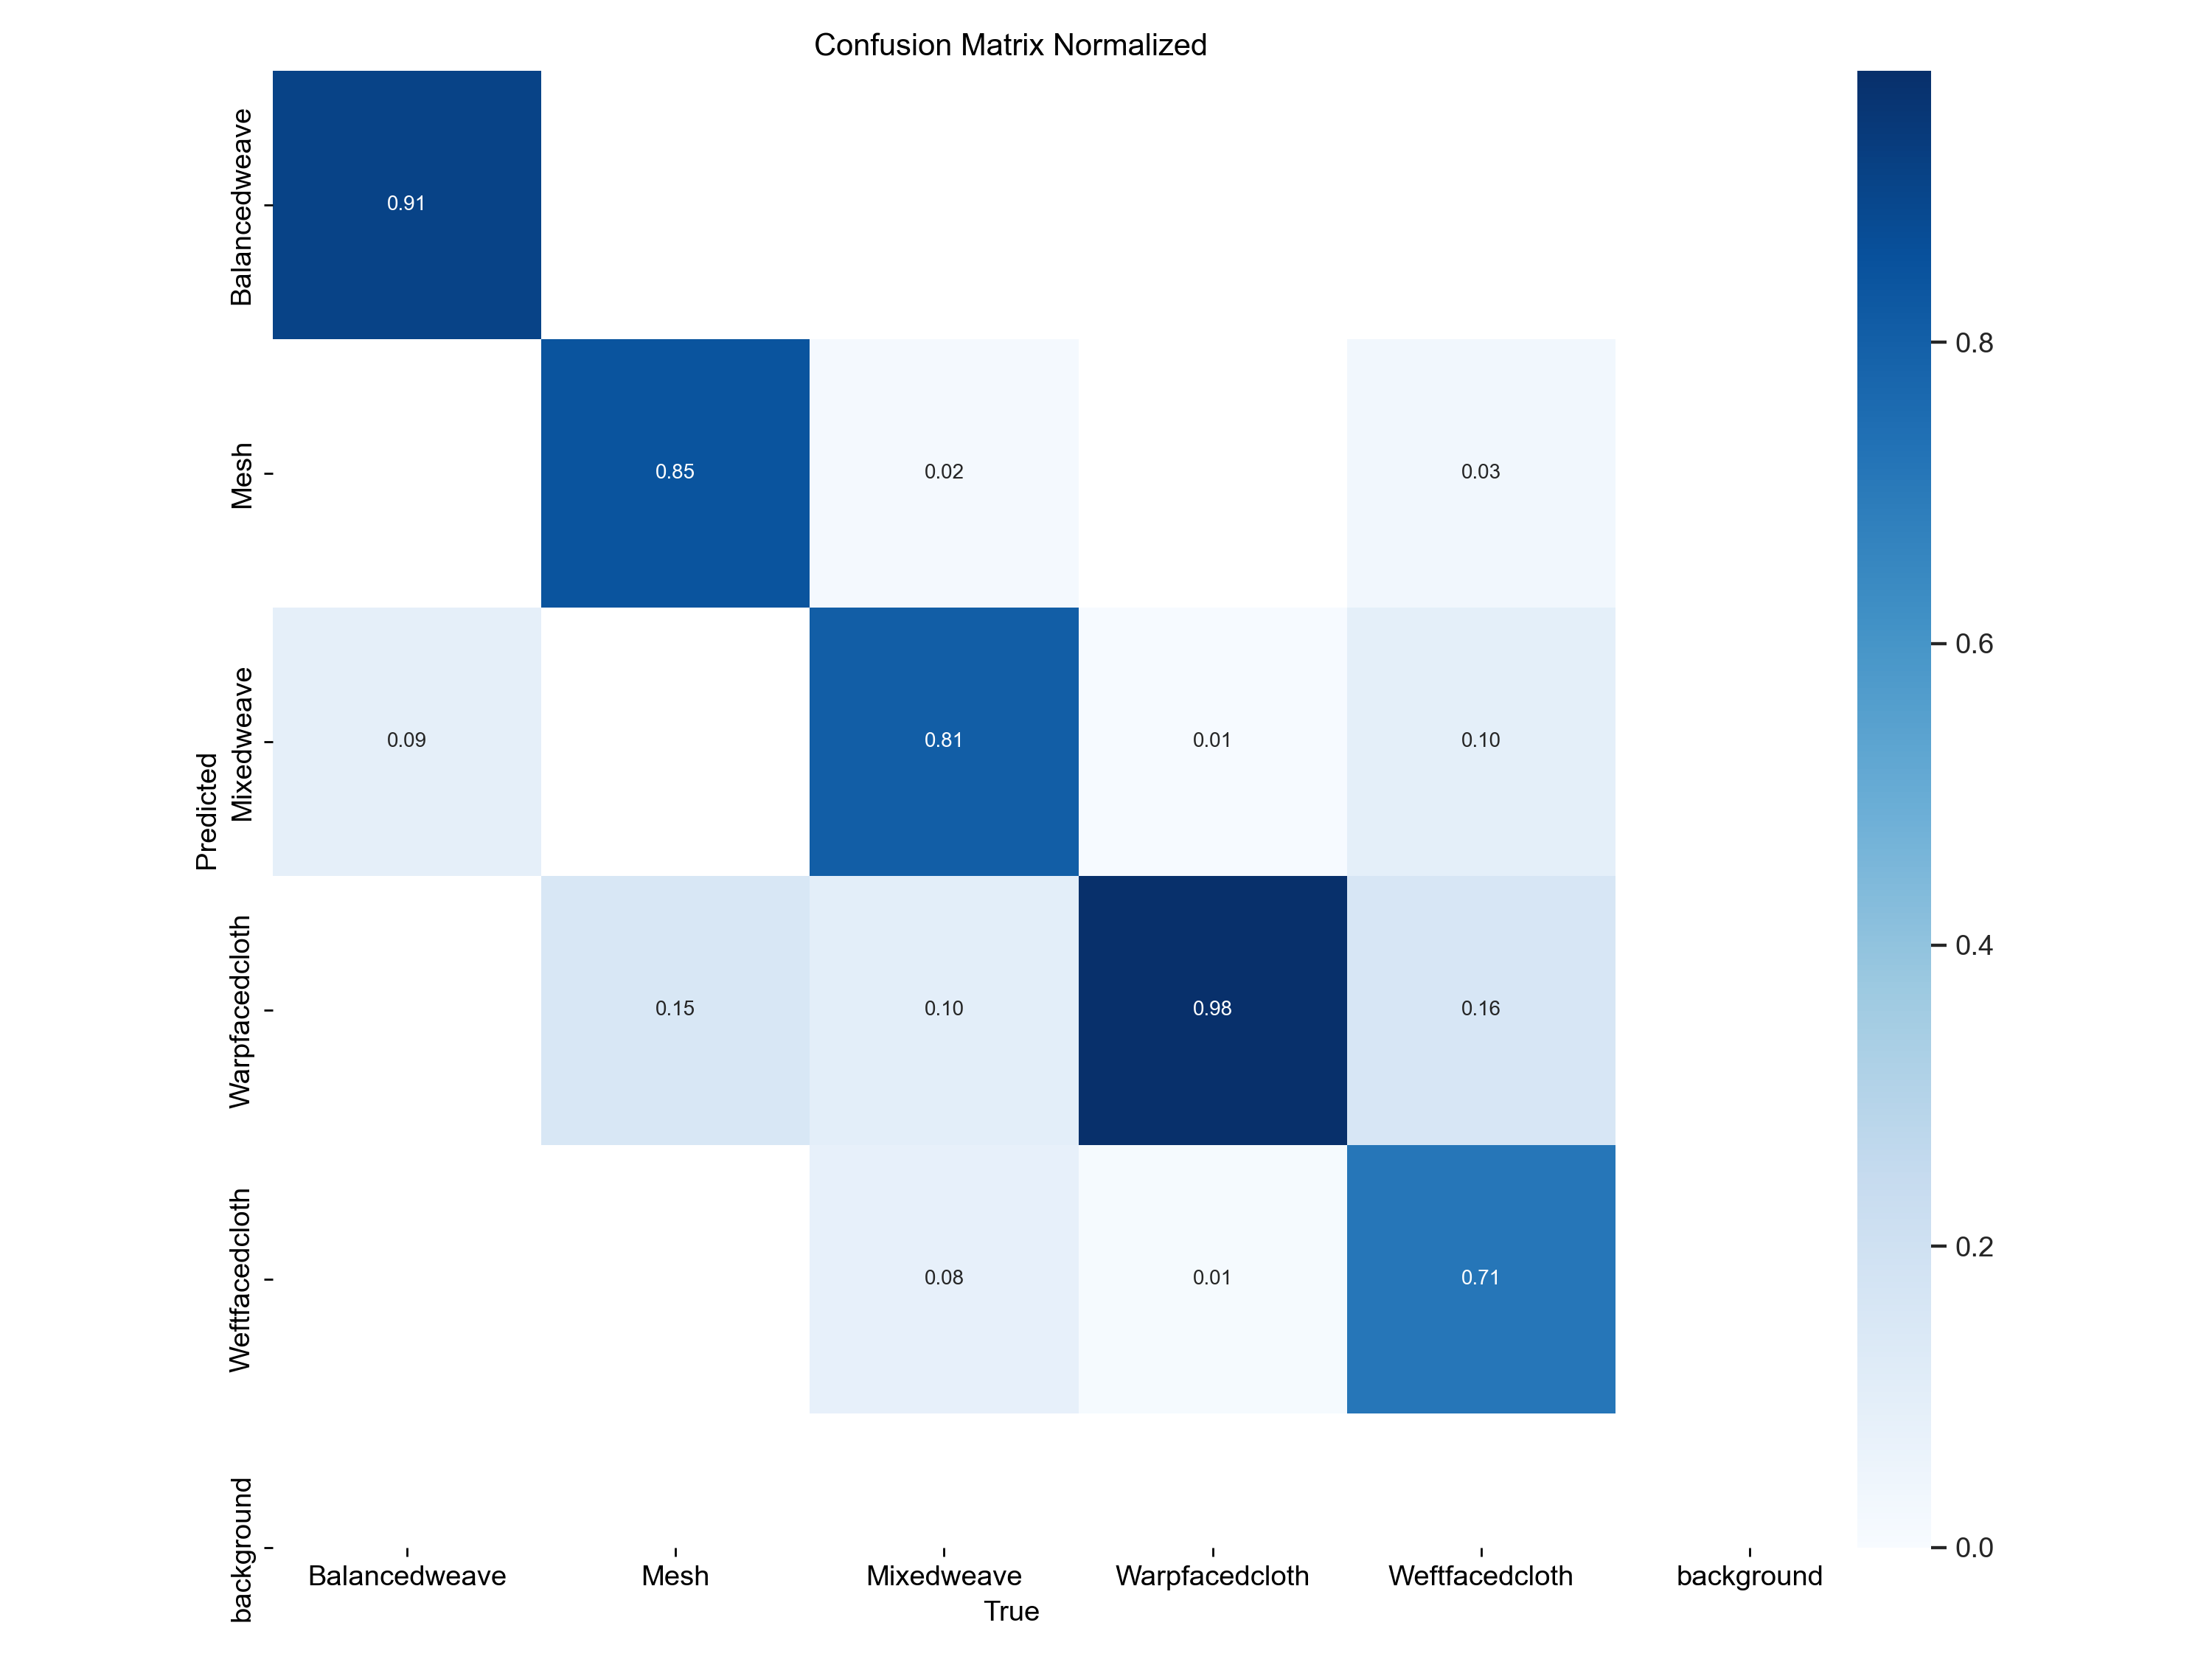
\includegraphics[width=16cm]{../images/YOLO_50epoch_confusion_matrix_normalized.png}
		\caption{Matrice de confusion du premier entraînement YOLO.}
	 \end{center}
\end{figure}

\begin{figure}[!h]
	\begin{center}
		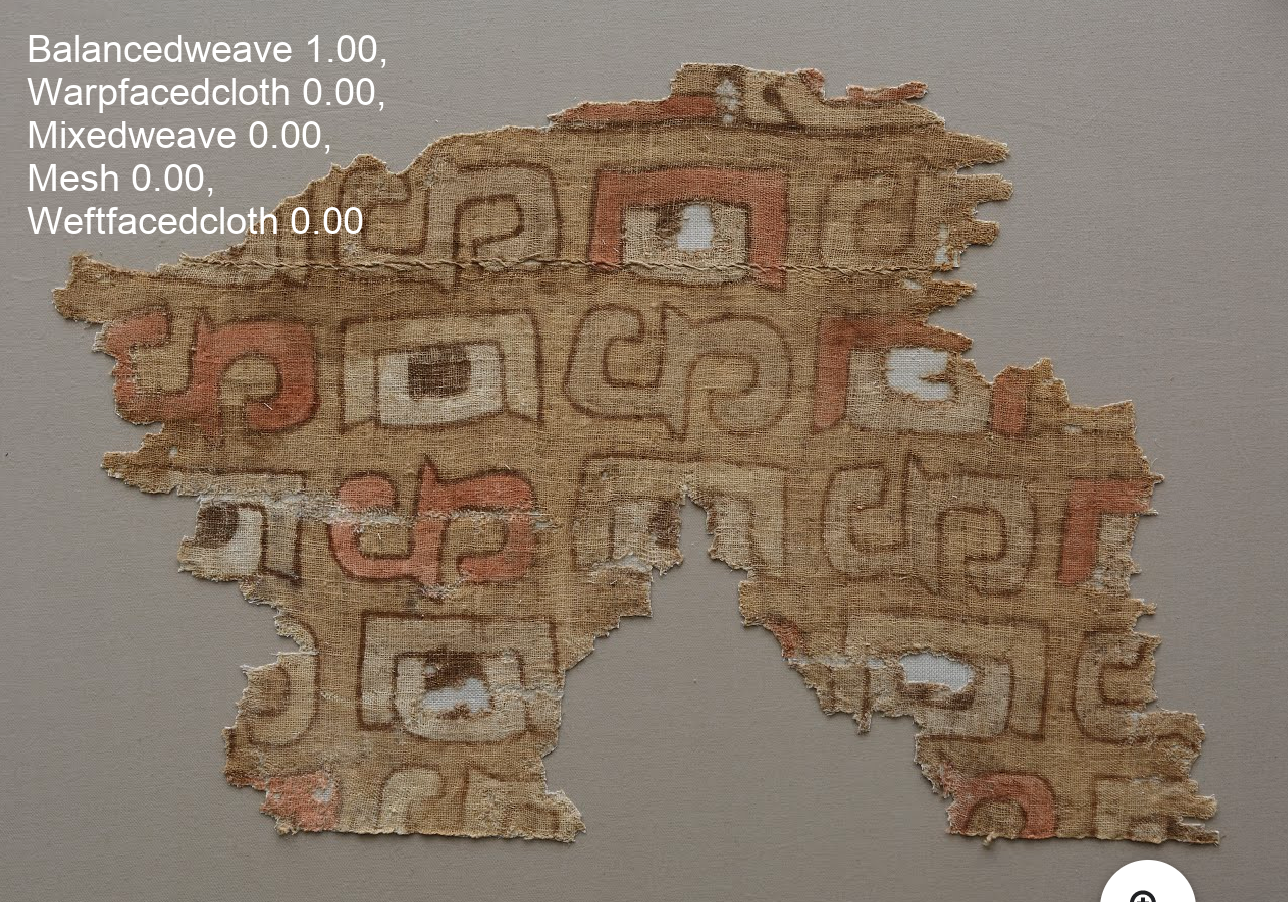
\includegraphics[width=7cm]{../images/AMANObalancedWeave.png}
		\caption{Toile issue des collections du musée Amano.}
	 \end{center}
\end{figure}

\clearpage

\begin{figure}[!h]
 \begin{minipage}[c]{.5\linewidth}
        \begin{center}
        		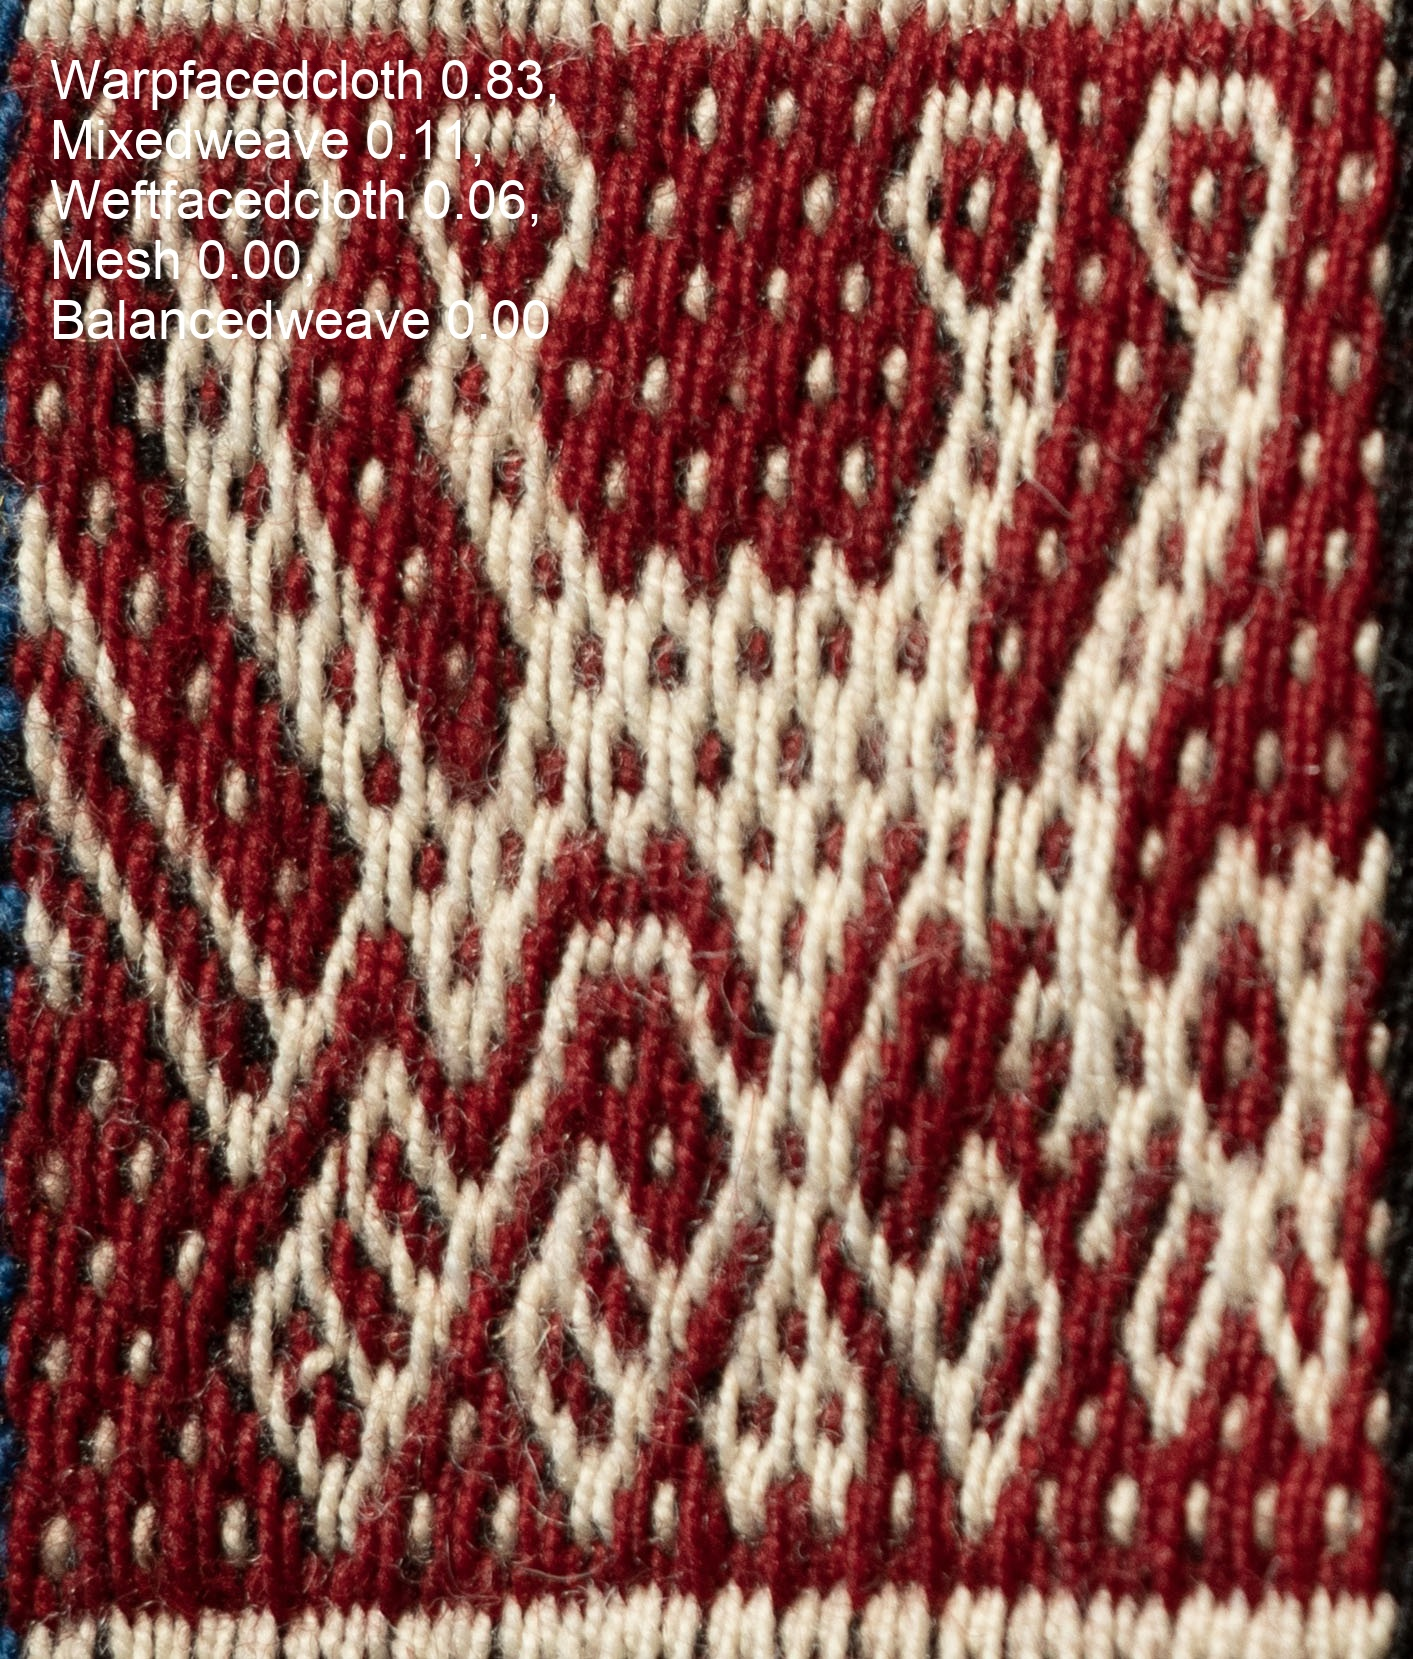
\includegraphics[height=6cm]{../images/weave1.jpg}
	\end{center}
    \end{minipage}
            \begin{minipage}[c]{.5\linewidth}
        \begin{center}
        		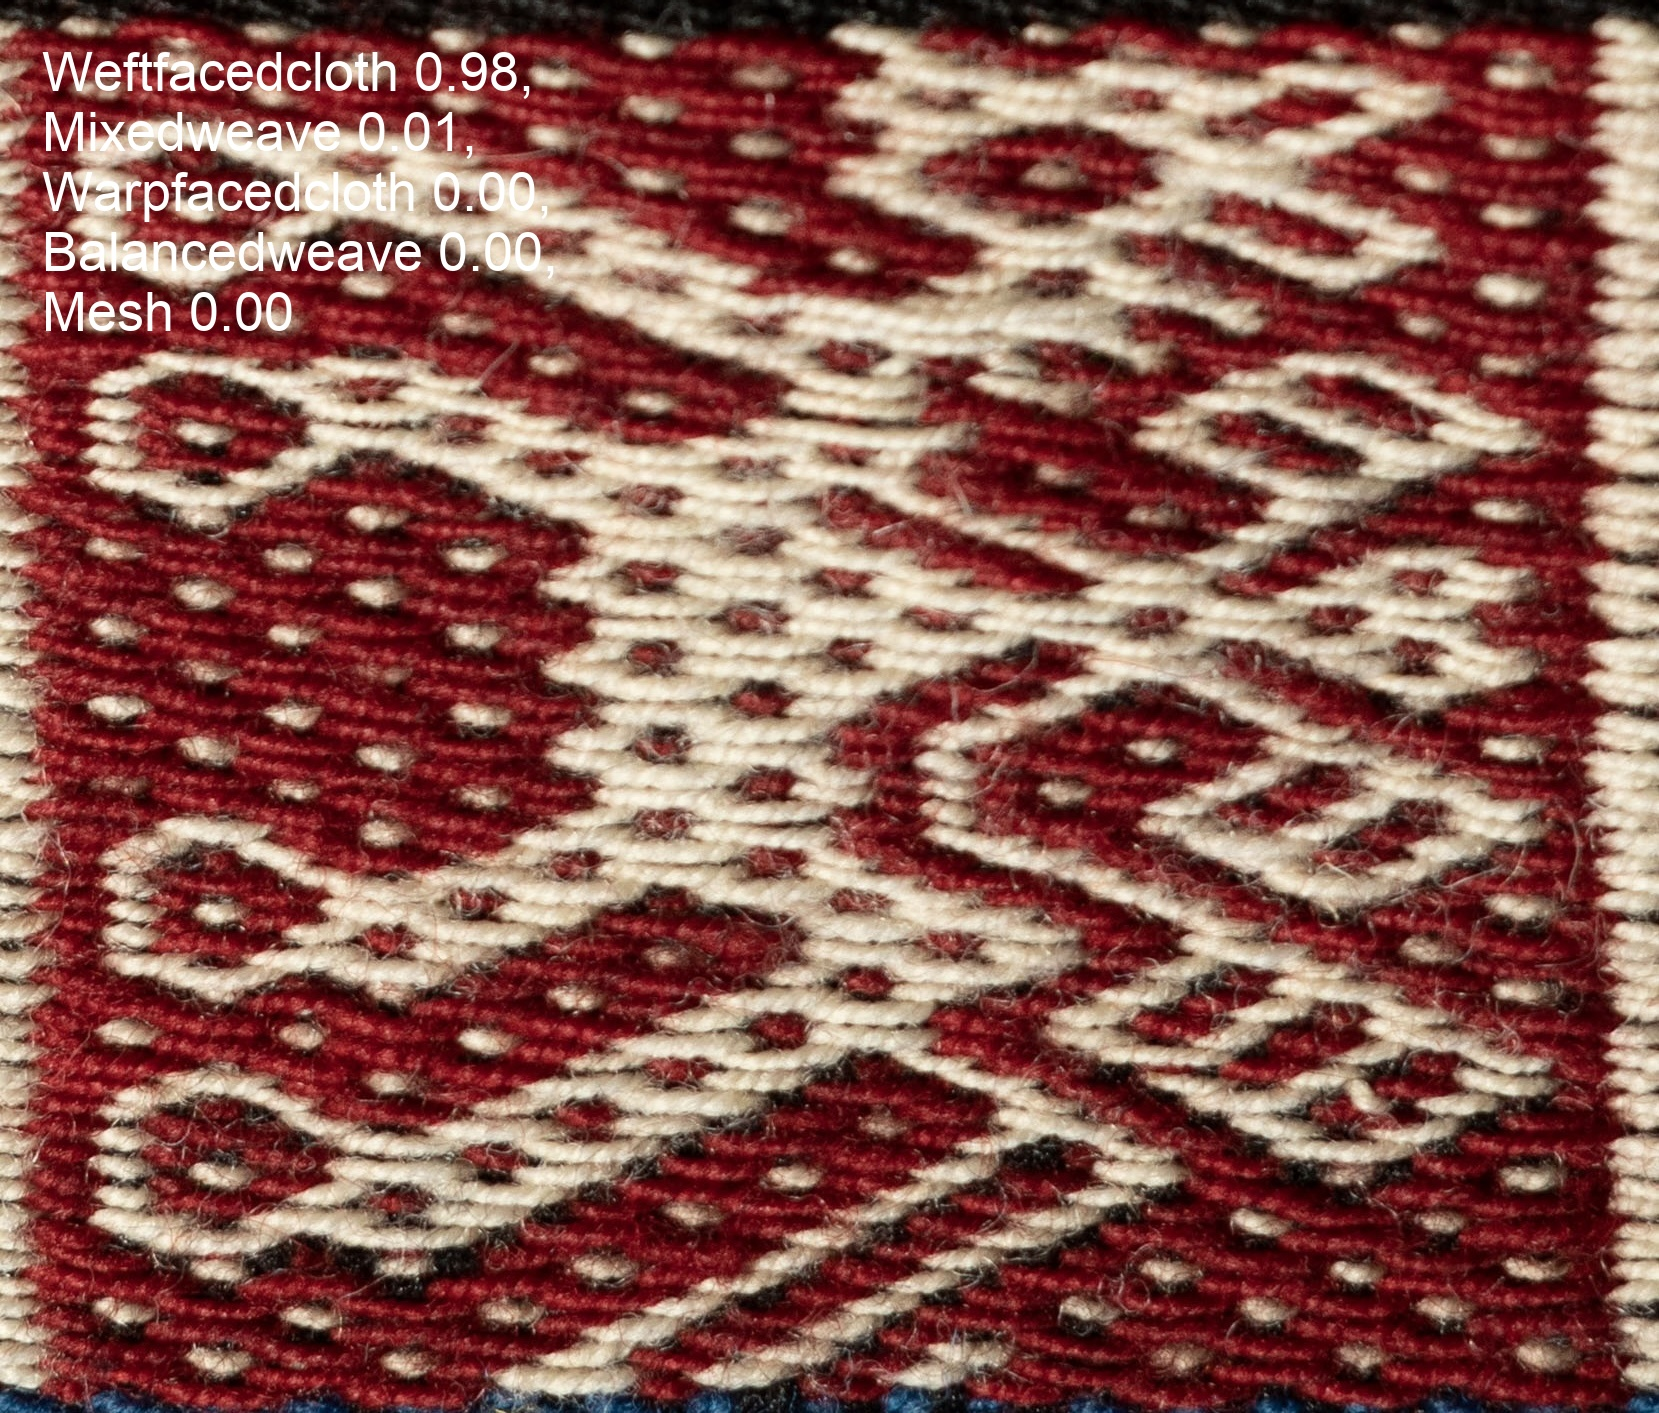
\includegraphics[height=6cm]{../images/weave1r.jpg}
	\end{center}
    \end{minipage}
    \caption{Détail d'un tissage à dominante chaîne orienté différemment.}
\end{figure}

\subsubsection{Classification à partir d'un dataset équilibré.}

\begin{table}[!h]
    \centering
    \begin{tabular}{|c|c|c|}
        \hline
         \cellcolor{blue!20}\textbf{Technique} & \cellcolor{blue!20}\textbf{Nombre d'images}& \cellcolor{blue!20} \textbf{Pourcentage} \\ \hline \hline
         Warp-faced cloth & 54 & 20\% \\ \hline
         Weft-faced cloth & 54  &20\% \\ \hline
         Balanced weave & 54 & 20\% \\ \hline
         Mixed Weave & 54 &  20\% \\ \hline
         Mesh & 54 & 20\% \\ \hline
         \textbf{Total} & \textbf{270} &  \textbf{100\%}  \\ \hline
    \end{tabular}
    \caption{Répartition des classes dans un dataset équilibré.}
    \label{tab:classes_eq}
\end{table}

\begin{figure}[!h]
    \begin{minipage}[c]{.4\linewidth}
            \begin{center}
                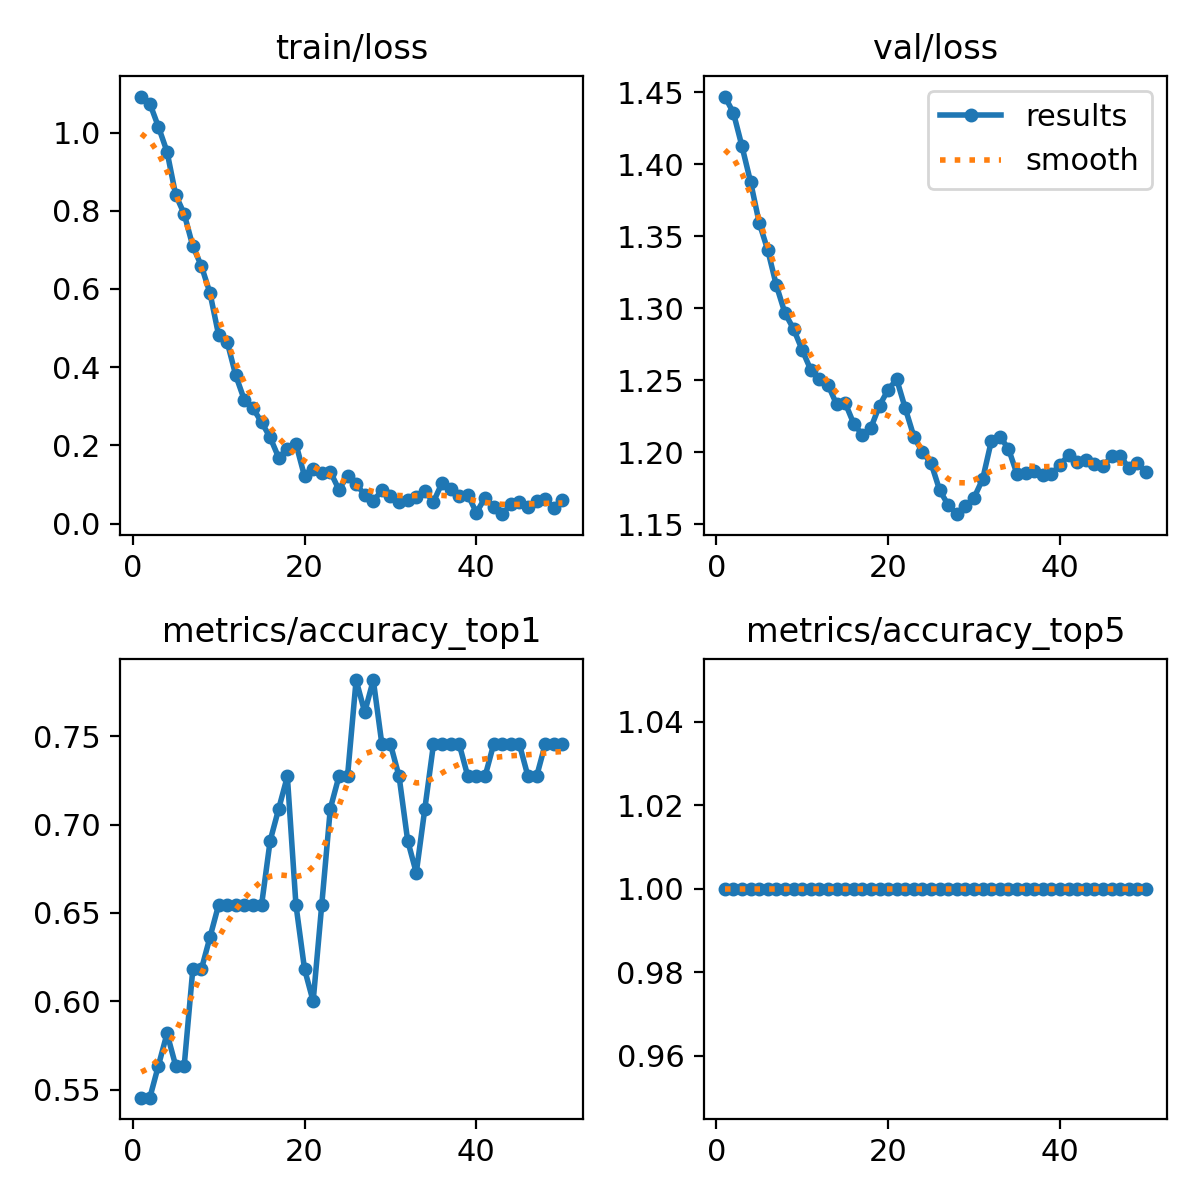
\includegraphics[height=6cm]{../images/YOLO_50epoch_eq.png}
            \end{center}
    \end{minipage}
        \begin{minipage}[c]{.6\linewidth}
        \begin{center}
        		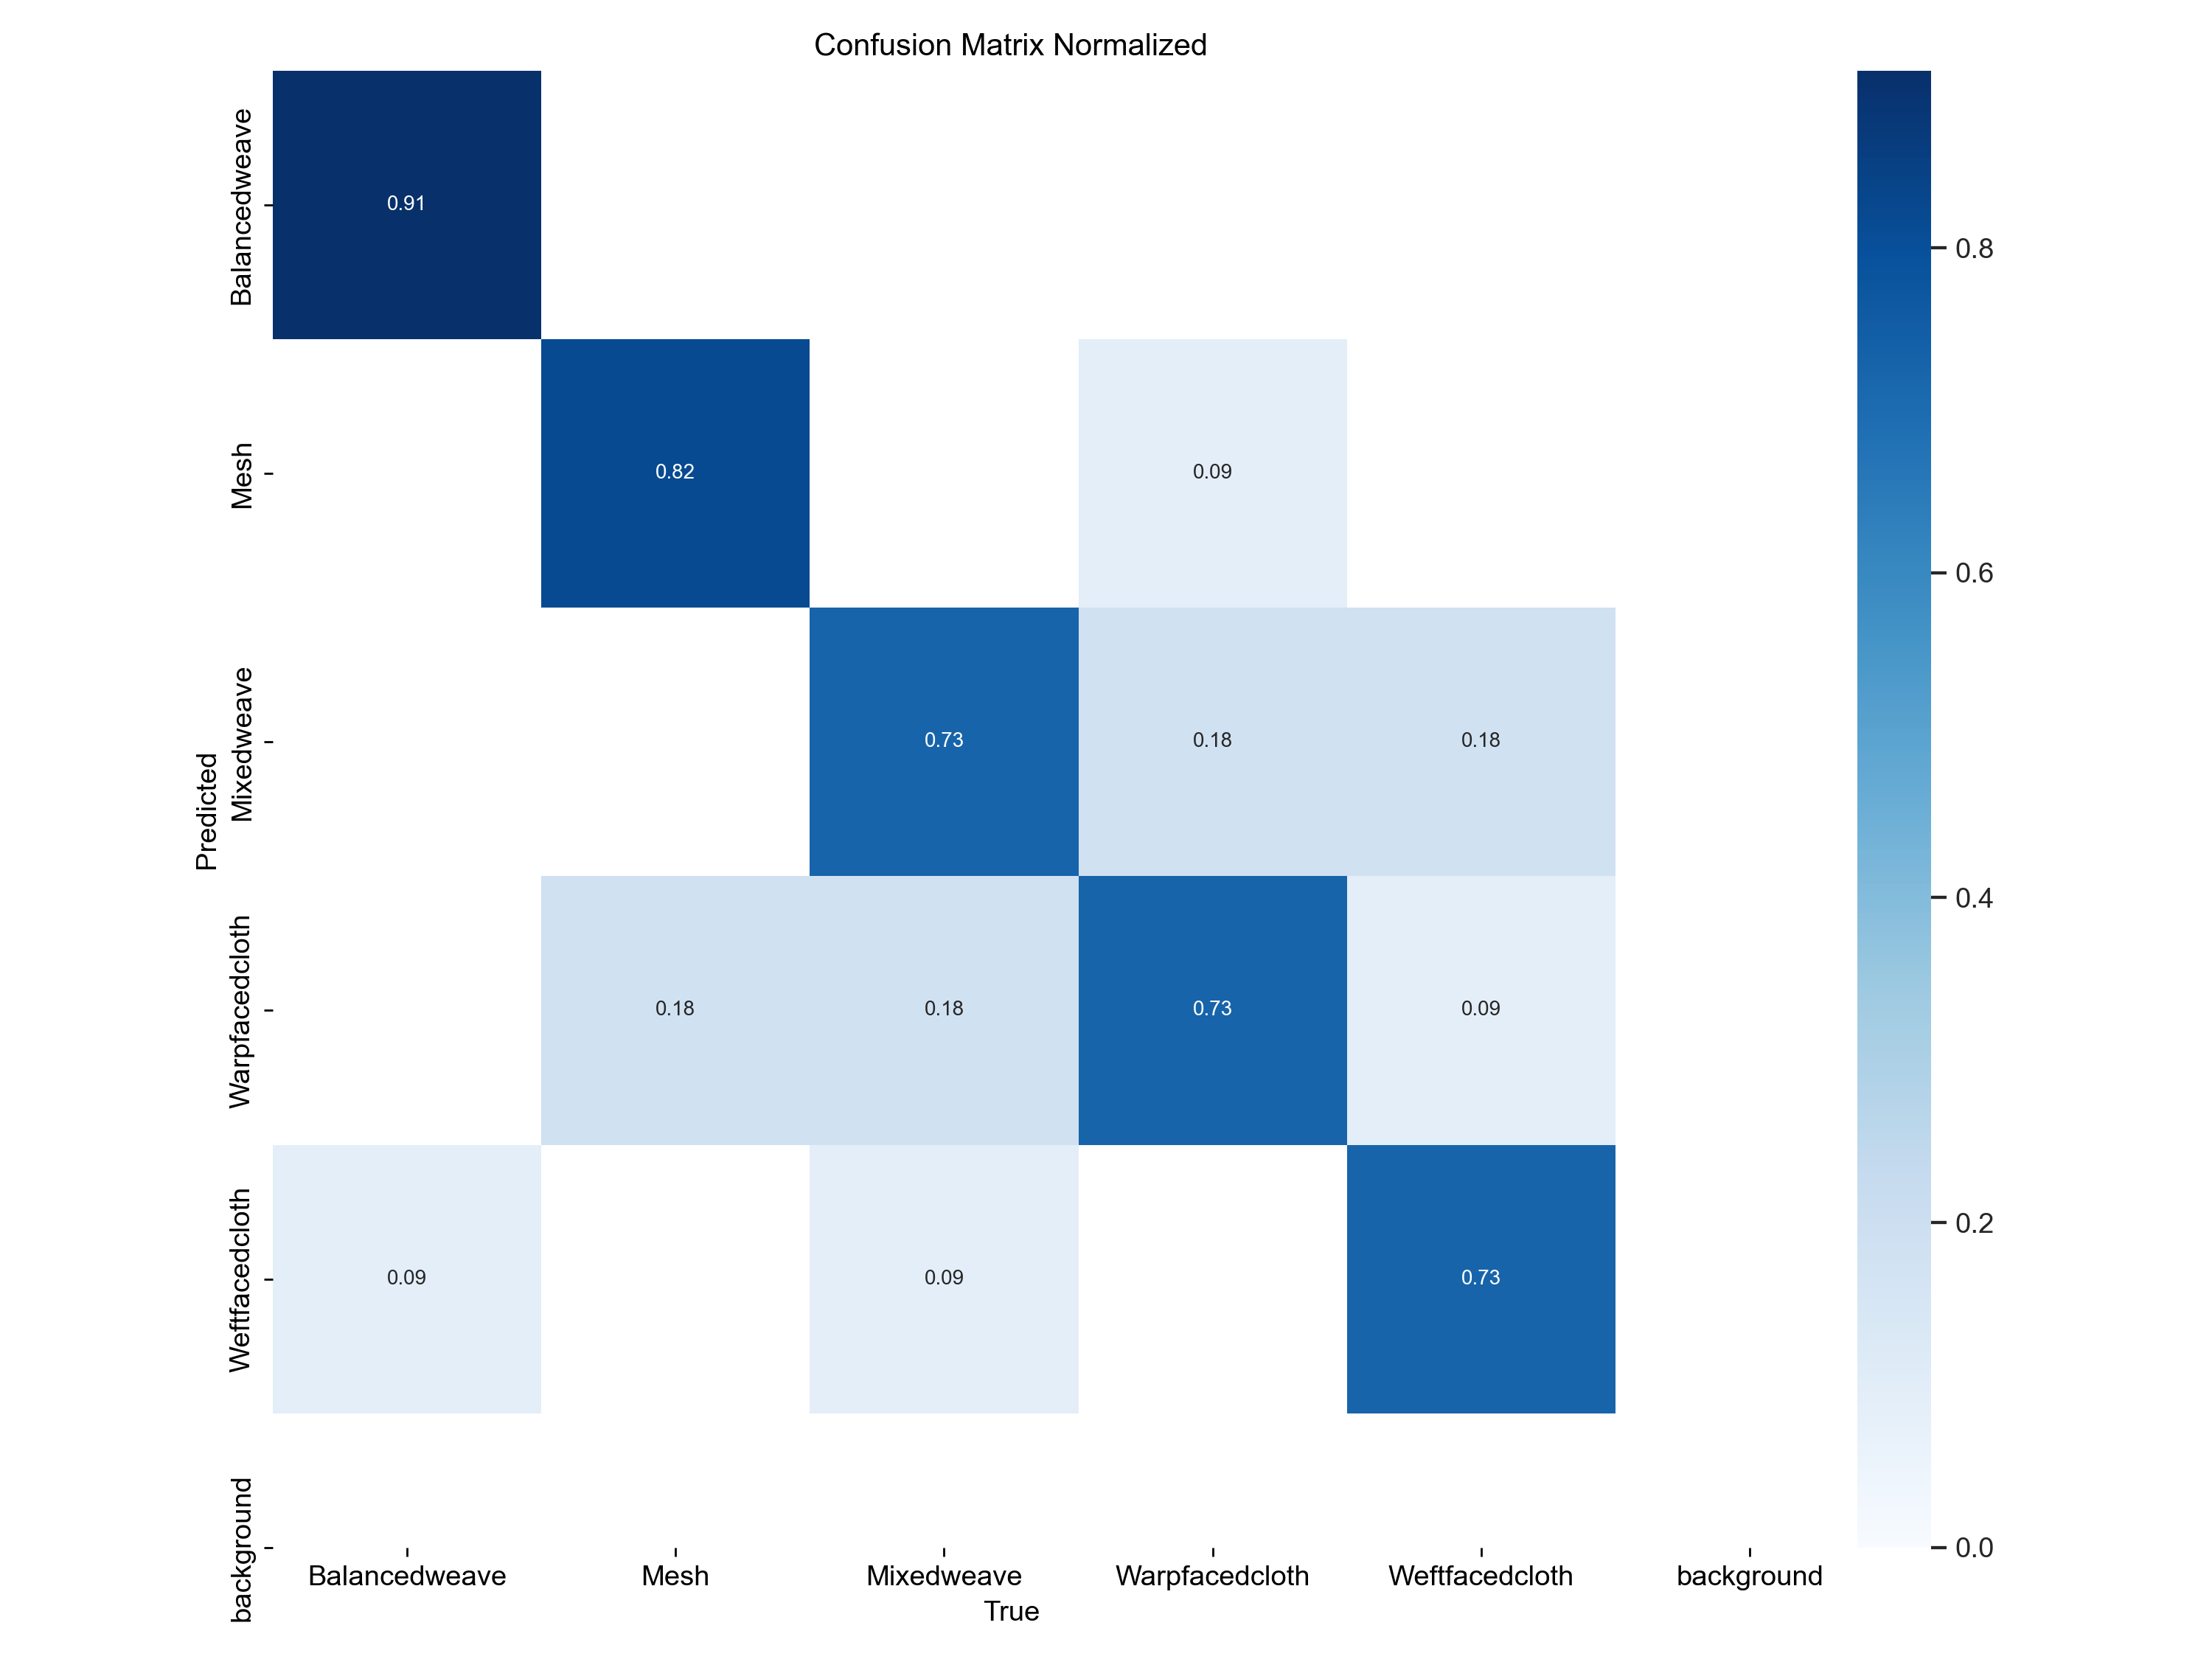
\includegraphics[height=9cm]{../images/YOLO_50epoch_eq_confusion_matrix_normalized.png}
	\end{center}
    \end{minipage}
    \caption{Résultats du second entraînement YOLO (courbes de précision, d'apprentissage et matrice de confusion).}
    \label{fig:YOLO_eq}   
\end{figure}

Face à ces biais, nous avons réalisé une seconde tentative d'entraînement à partir d'un \textit{dataset} équilibré, c'est-à-dire qui contient le même nombre d'images pour chaque catégorie entraînée. Pour cela, nous avons réduit les images d'entraînement à 54 par classes, nombre d'images disponibles pour la classe la moins dotée. Ce second entraînement utilise 270 images. L'entraînement se fait en 50 époques, avec des \textit{batchs} de 32 images et un \textit{dropout} de 0,1. Nous passons à 32 images par \textit{batch} pour réduire le temps de calcul du modèle.

La précision du modèle atteint son maximum à la $26^{eme}$ époque avec 78,18\% de précision, ensuite elle diminue pour alterner entre deux paliers de 72\% et 74\% de précision. Les résultats sont moins bons que le premier entraînement, avec une plus grande confusion entre les classes tissages mixtes, tissages à dominante chaîne et tissages à dominante trame. Toutefois, cette erreur semble cohérente puisqu'il s'agit de trois techniques à l'aspect proche. La catégorie tissage à dominante trame est la mieux détectée après l'équilibrage du \textit{dataset}.

\begin{figure}[!h]
	\begin{center}
		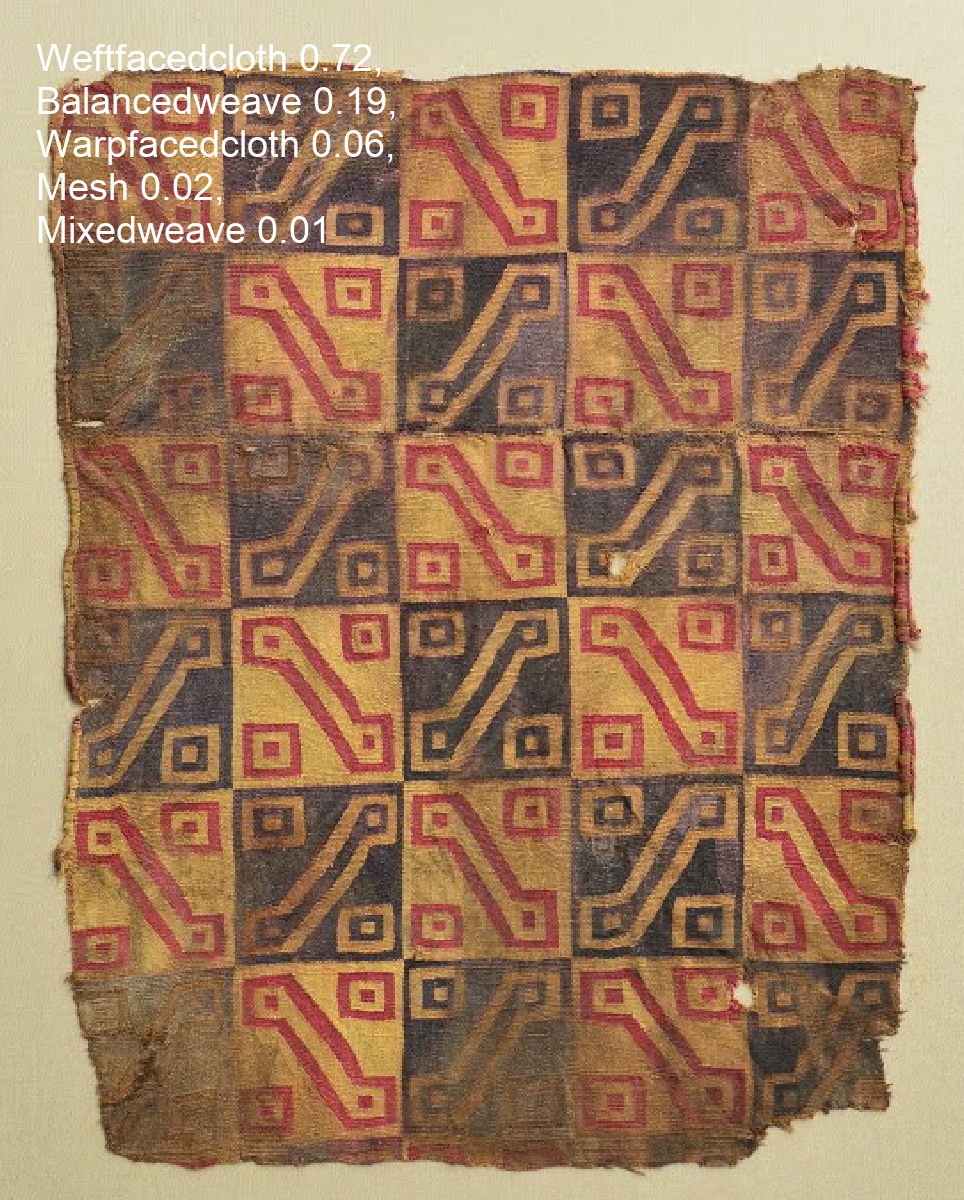
\includegraphics[width=5cm]{../images/AMANOweft2.png}
		\caption{Tissage à dominante trame issue des collections du musée Amano.}
	 \end{center}
\end{figure}

\subsubsection{Classification à partir d'un dataset augmenté et équilibré.}

Pour améliorer les résultats du modèle, nous décidons de garder un \textit{dataset} équilibré, tout en augmentant le nombre d'échantillons fournis au modèle, ce qui semble permettre une meilleure précision globale. Pour cela, nous avons recours à un processus d'augmentation des données c'est-à-dire l'accroissement artificiel de la quantité de données d'apprentissage\footnote{Cette méthode est inspirée par la proposition de Mike Kestemont dans le cadre du projet DeepScript qui visait à classifier les écritures manuscrites médiévales. Voir : \url{https://github.com/mikekestemont/DeepScript/tree/master?tab=readme-ov-file}.}. L'idée est d'extraire des \textit{patchs}, morceaux d'images, issus du \textit{dataset} que l'on modifie pour ne pas sur-entraîner le modèle. Nous avons donc extrait des \textit{patchs} (recouvrant un quart de l'image originale) pour les deux classes les moins dotées, ces \textit{patchs} ont ensuite été modifiés suivant une symétrie axiale.


\begin{table}[!h]
    \centering
    \begin{tabular}{|c|c|c|}
        \hline
         \cellcolor{blue!20}\textbf{Technique} & \cellcolor{blue!20}\textbf{Nombre d'images}& \cellcolor{blue!20} \textbf{Pourcentage} \\ \hline \hline
         Warp-faced cloth & 216 & 20\% \\ \hline
         Weft-faced cloth & 216 & 20\% \\ \hline
         Balanced weave & 216 & 20\% \\ \hline
         Mixed Weave & 216 & 20\%  \\ \hline
         Mesh & 216 & 20\%  \\ \hline
         \textbf{Total} & \textbf{1080} &  \textbf{100\%}  \\ \hline
    \end{tabular}
    \caption{Répartition des classes dans un dataset équilibré et augmenté.}
    \label{tab:classes_eq_augment}
\end{table}

\noindent Par ailleurs, pour pallier le problème de l'orientation des fibres nous avons appliqué sur la totalité du \textit{dataset} des rotations de 0$^{\circ}$, 90$^{\circ}$, 180$^{\circ}$ et 360$^{\circ}$, ce qui signifie que la moitié des images du \textit{dataset} est pivotée et donc que l'orientation de ses fils est modifiée.

Dans ce cas nous avons 216 images par classes, nombres d'images disponibles pour la classe la moins dotée. L'entraînement se fait alors en 50 époques sur 1320 images regroupées en \textit{batchs} de 32 images avec un \textit{dropout} de 0,1. La précision du modèle atteint son maximum à la $46^{eme}$ époque avec 90,78\% de précision. La précision est supérieure à 85\% pour chaque catégorie.

\begin{figure}[!h]
    \begin{minipage}[c]{.4\linewidth}
            \begin{center}
                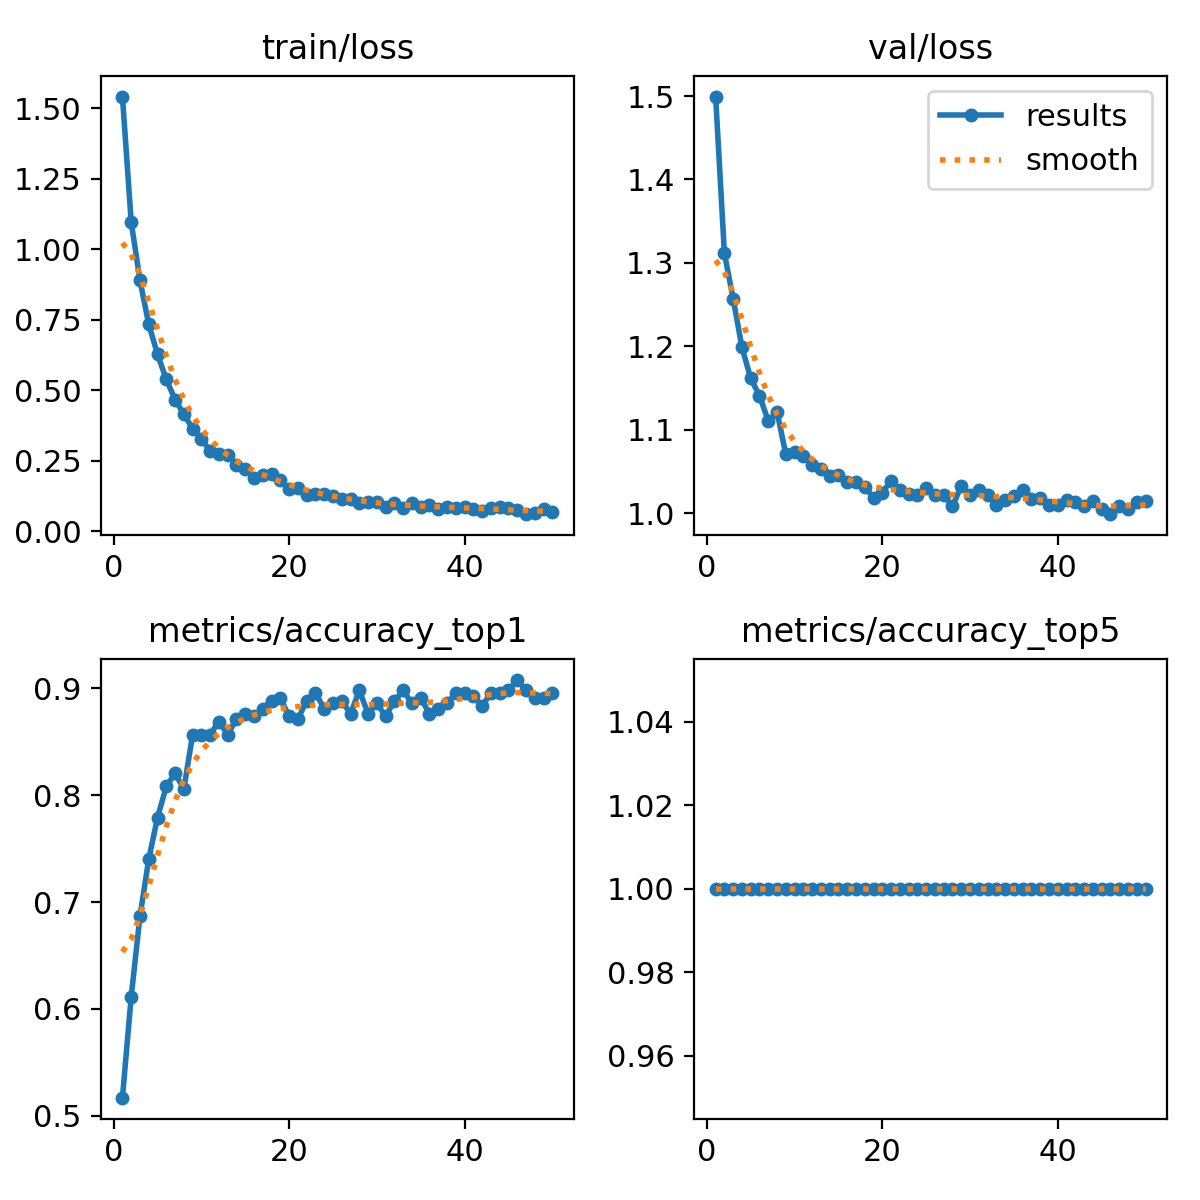
\includegraphics[height=6cm]{../images/YOLO_eq_augment.png}
            \end{center}
    \end{minipage}
        \begin{minipage}[c]{.6\linewidth}
        \begin{center}
        		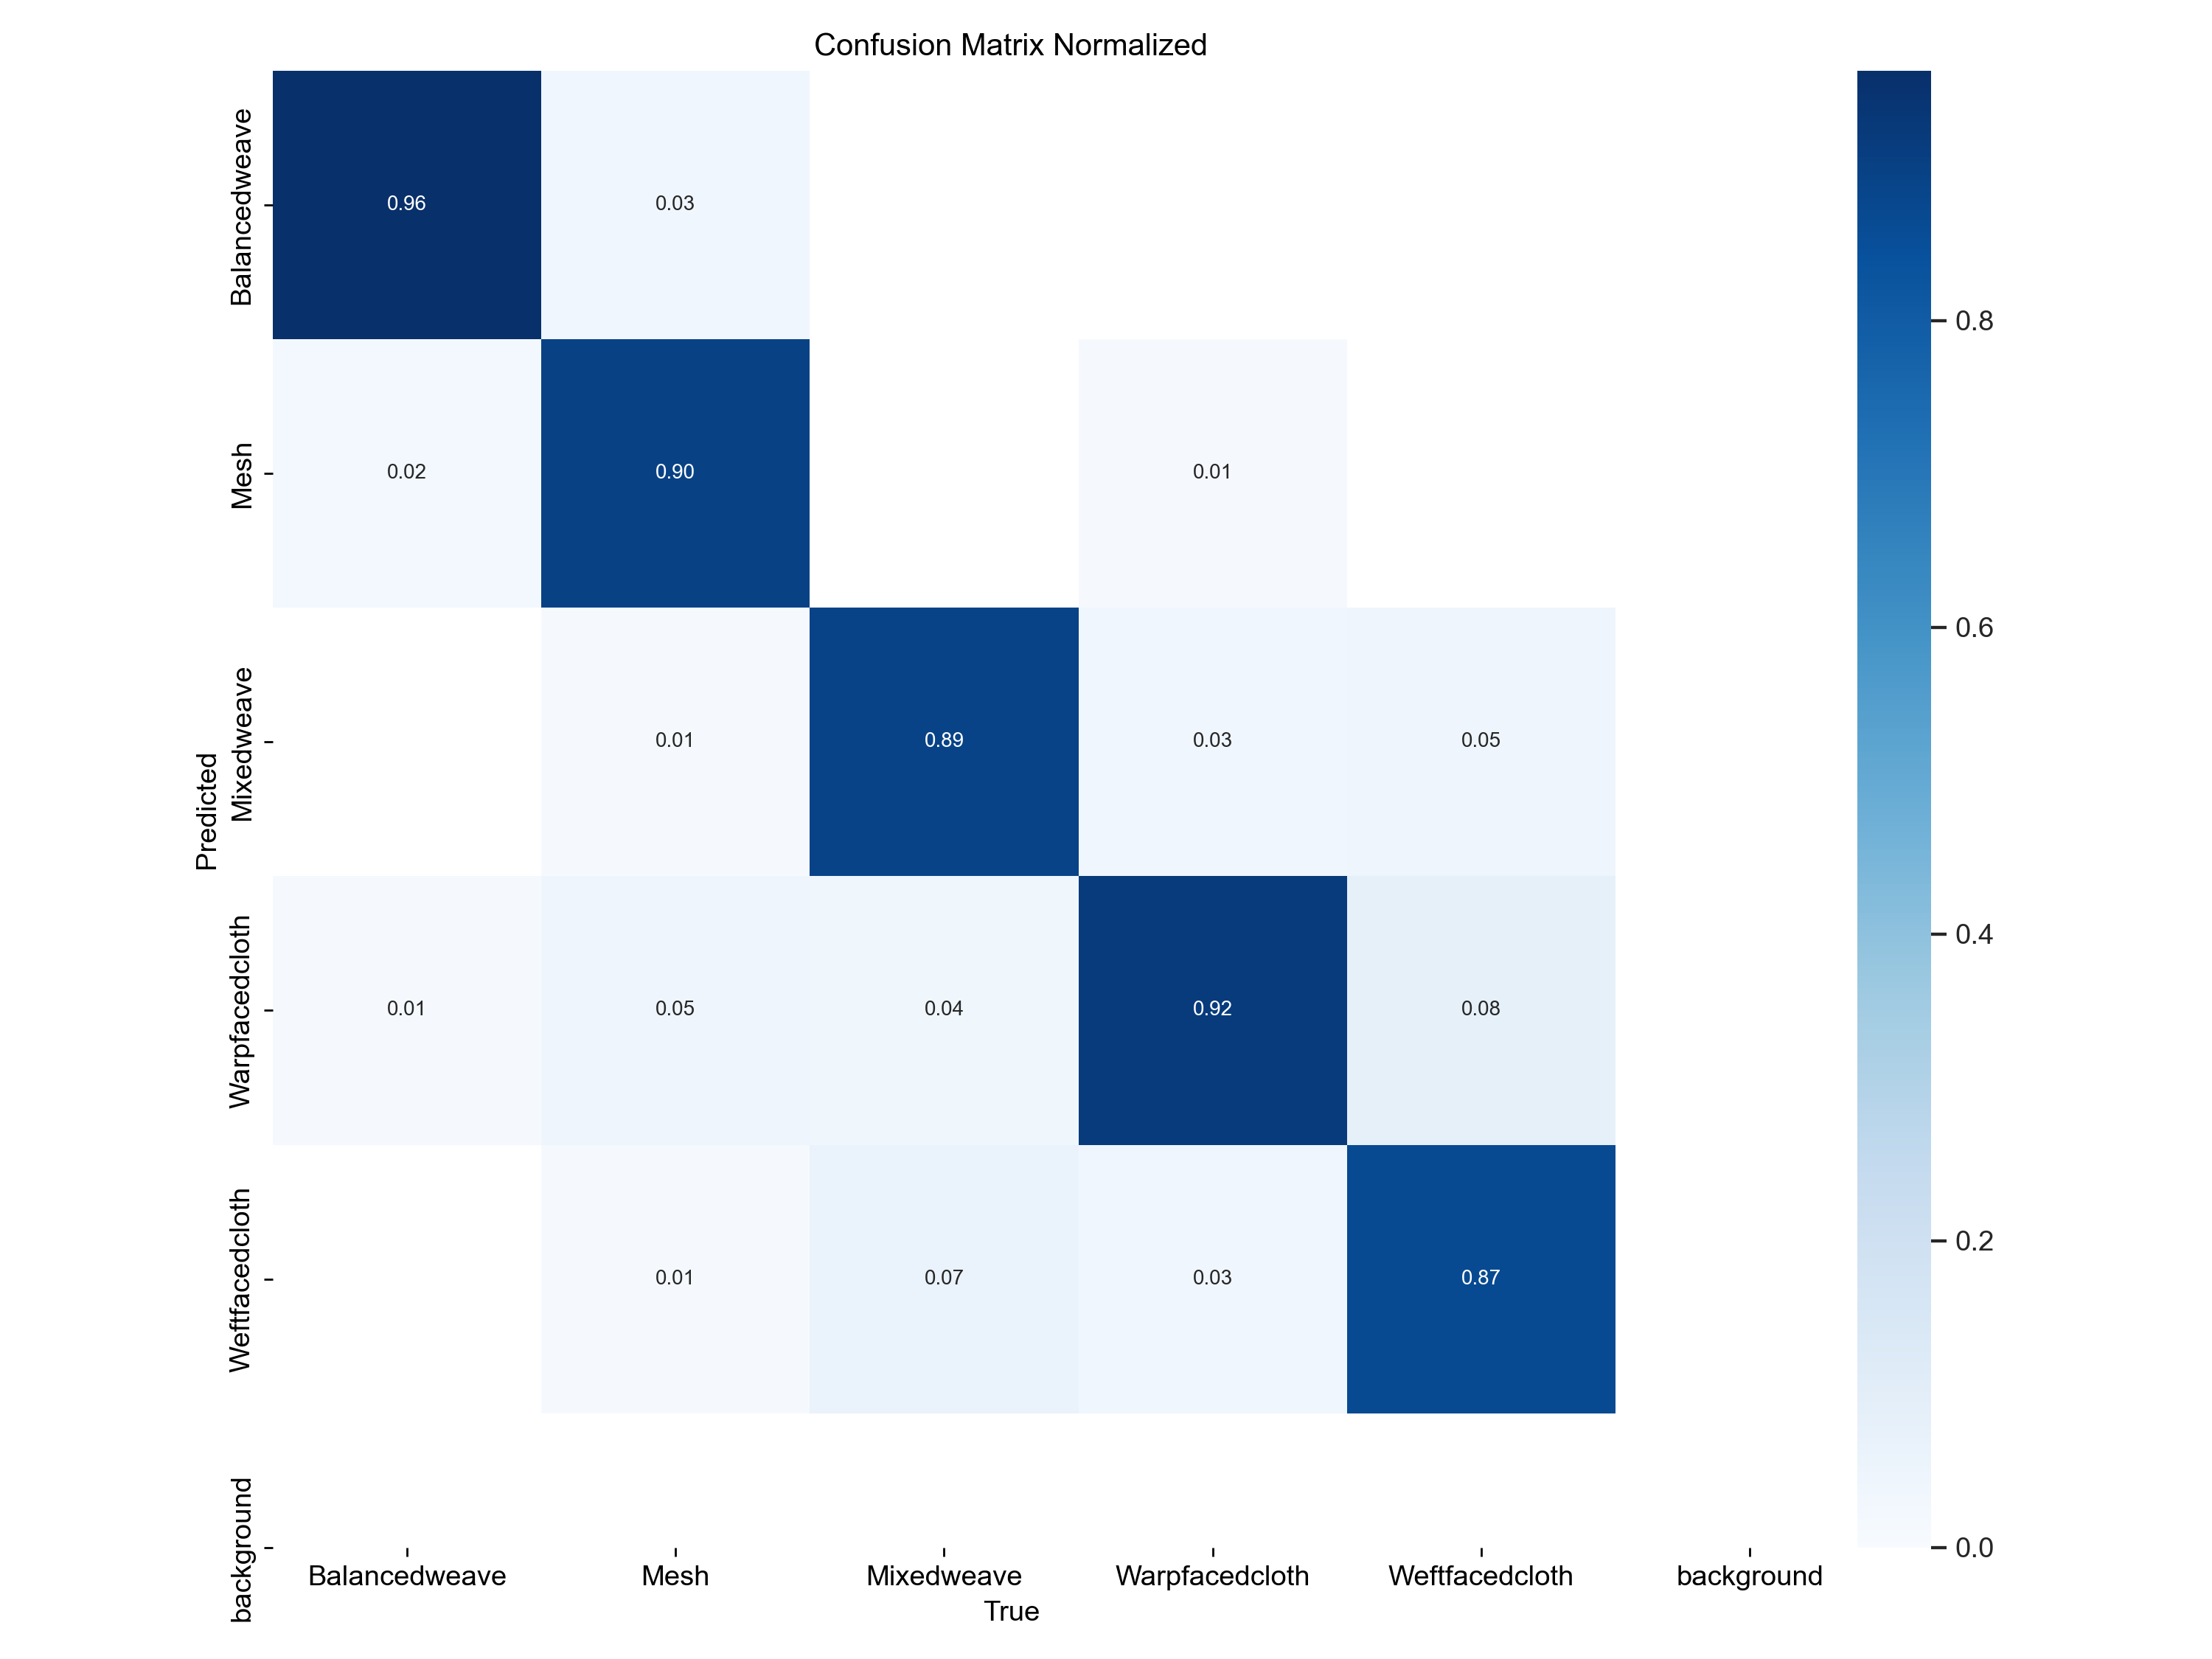
\includegraphics[height=9cm]{../images/YOLO_eq_augment_confusion_matrix_normalized.png}
	\end{center}
    \end{minipage}
    \caption{Résultats du second entraînement YOLO (courbes de précision, d'apprentissage et matrice de confusion).}
    \label{fig:YOLO_eq}   
\end{figure}

\begin{figure}[!h]
 \begin{minipage}[c]{.5\linewidth}
        \begin{center}
        		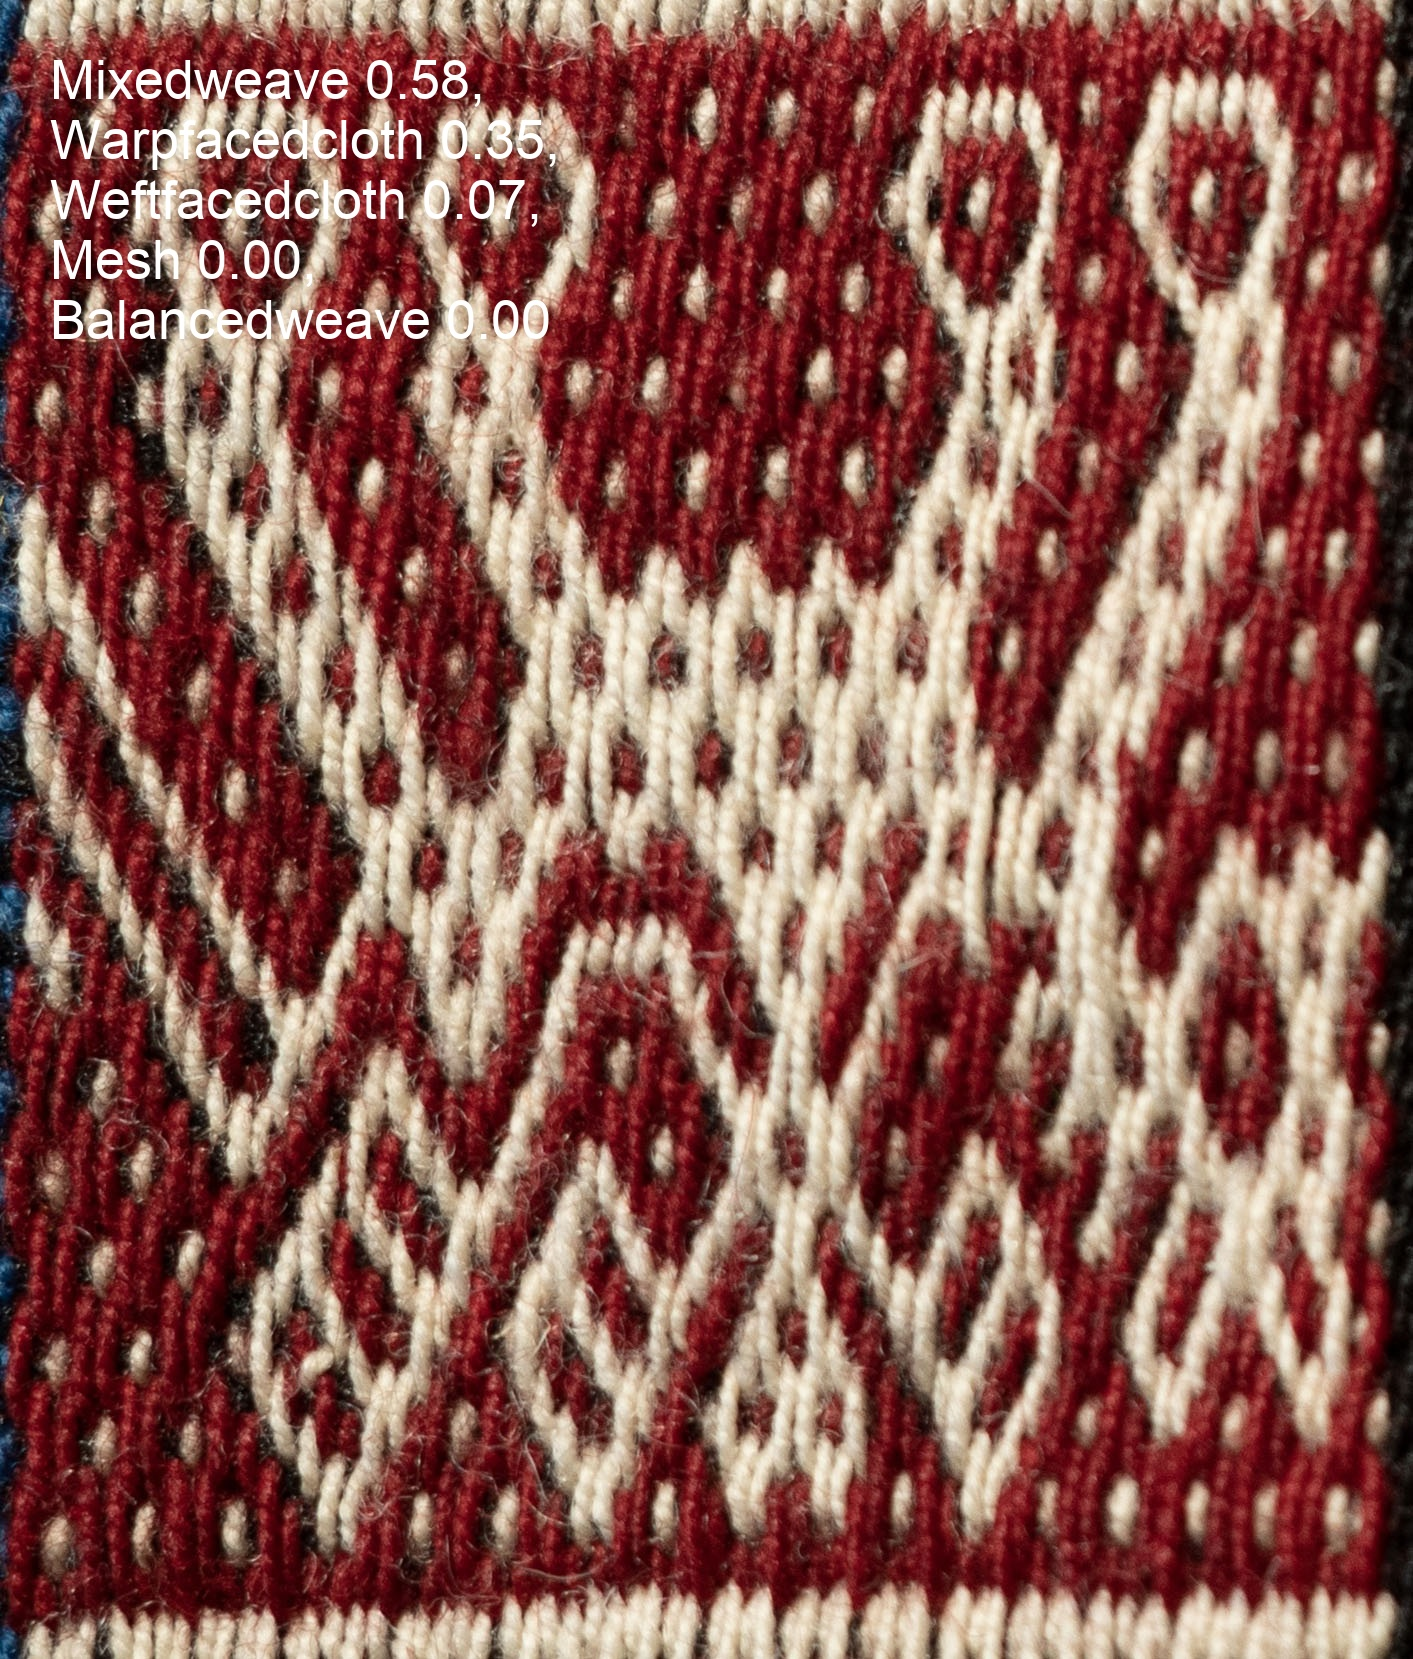
\includegraphics[height=6cm]{../images/weave1eqaugm.jpg}
	\end{center}
    \end{minipage}
            \begin{minipage}[c]{.5\linewidth}
        \begin{center}
        		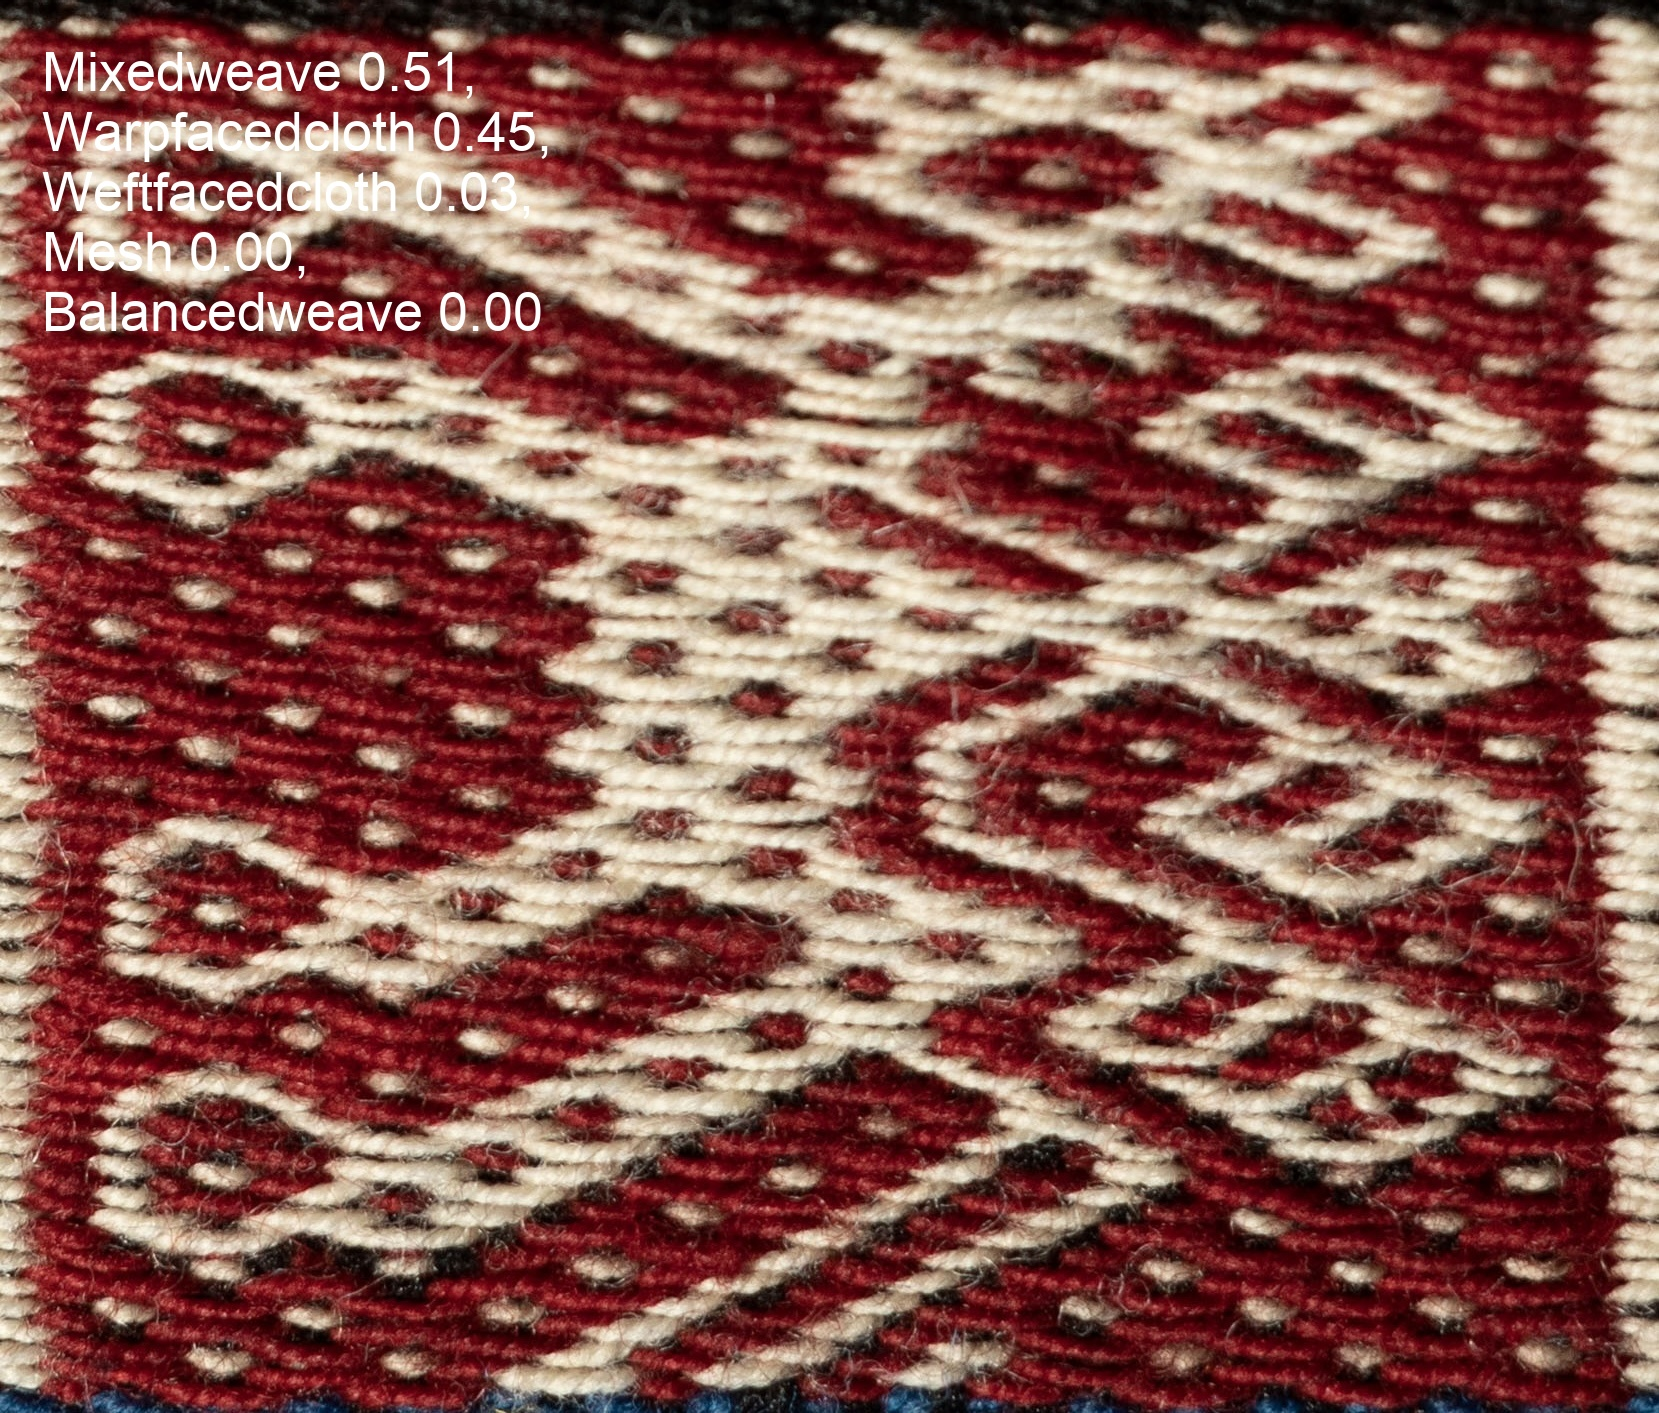
\includegraphics[height=6cm]{../images/weave1reqaugm.jpg}
	\end{center}
    \end{minipage}
    \caption{Détail d'un tissage à dominante chaîne orienté différemment.}
\end{figure}

En reprenant le même exemple de tissage à dominante chaîne, nous n'obtenons toujours pas la bonne catégorie même si cette fois-ci elle arrive en deuxième position dans les deux cas. Cependant, la variation du sens de la trame et de la chaîne n'a plus d'impact sur la classification. En prenant un seconde exemple de tissage à dominante chaîne, nous obtenons la bonne catégorie qui ne varie pas selon l'orientation des fibres. La rotation d'une partie des images du \textit{dataset} semble avoir pallié ce biais.

\begin{figure}[!h]
 \begin{minipage}[c]{.5\linewidth}
        \begin{center}
        		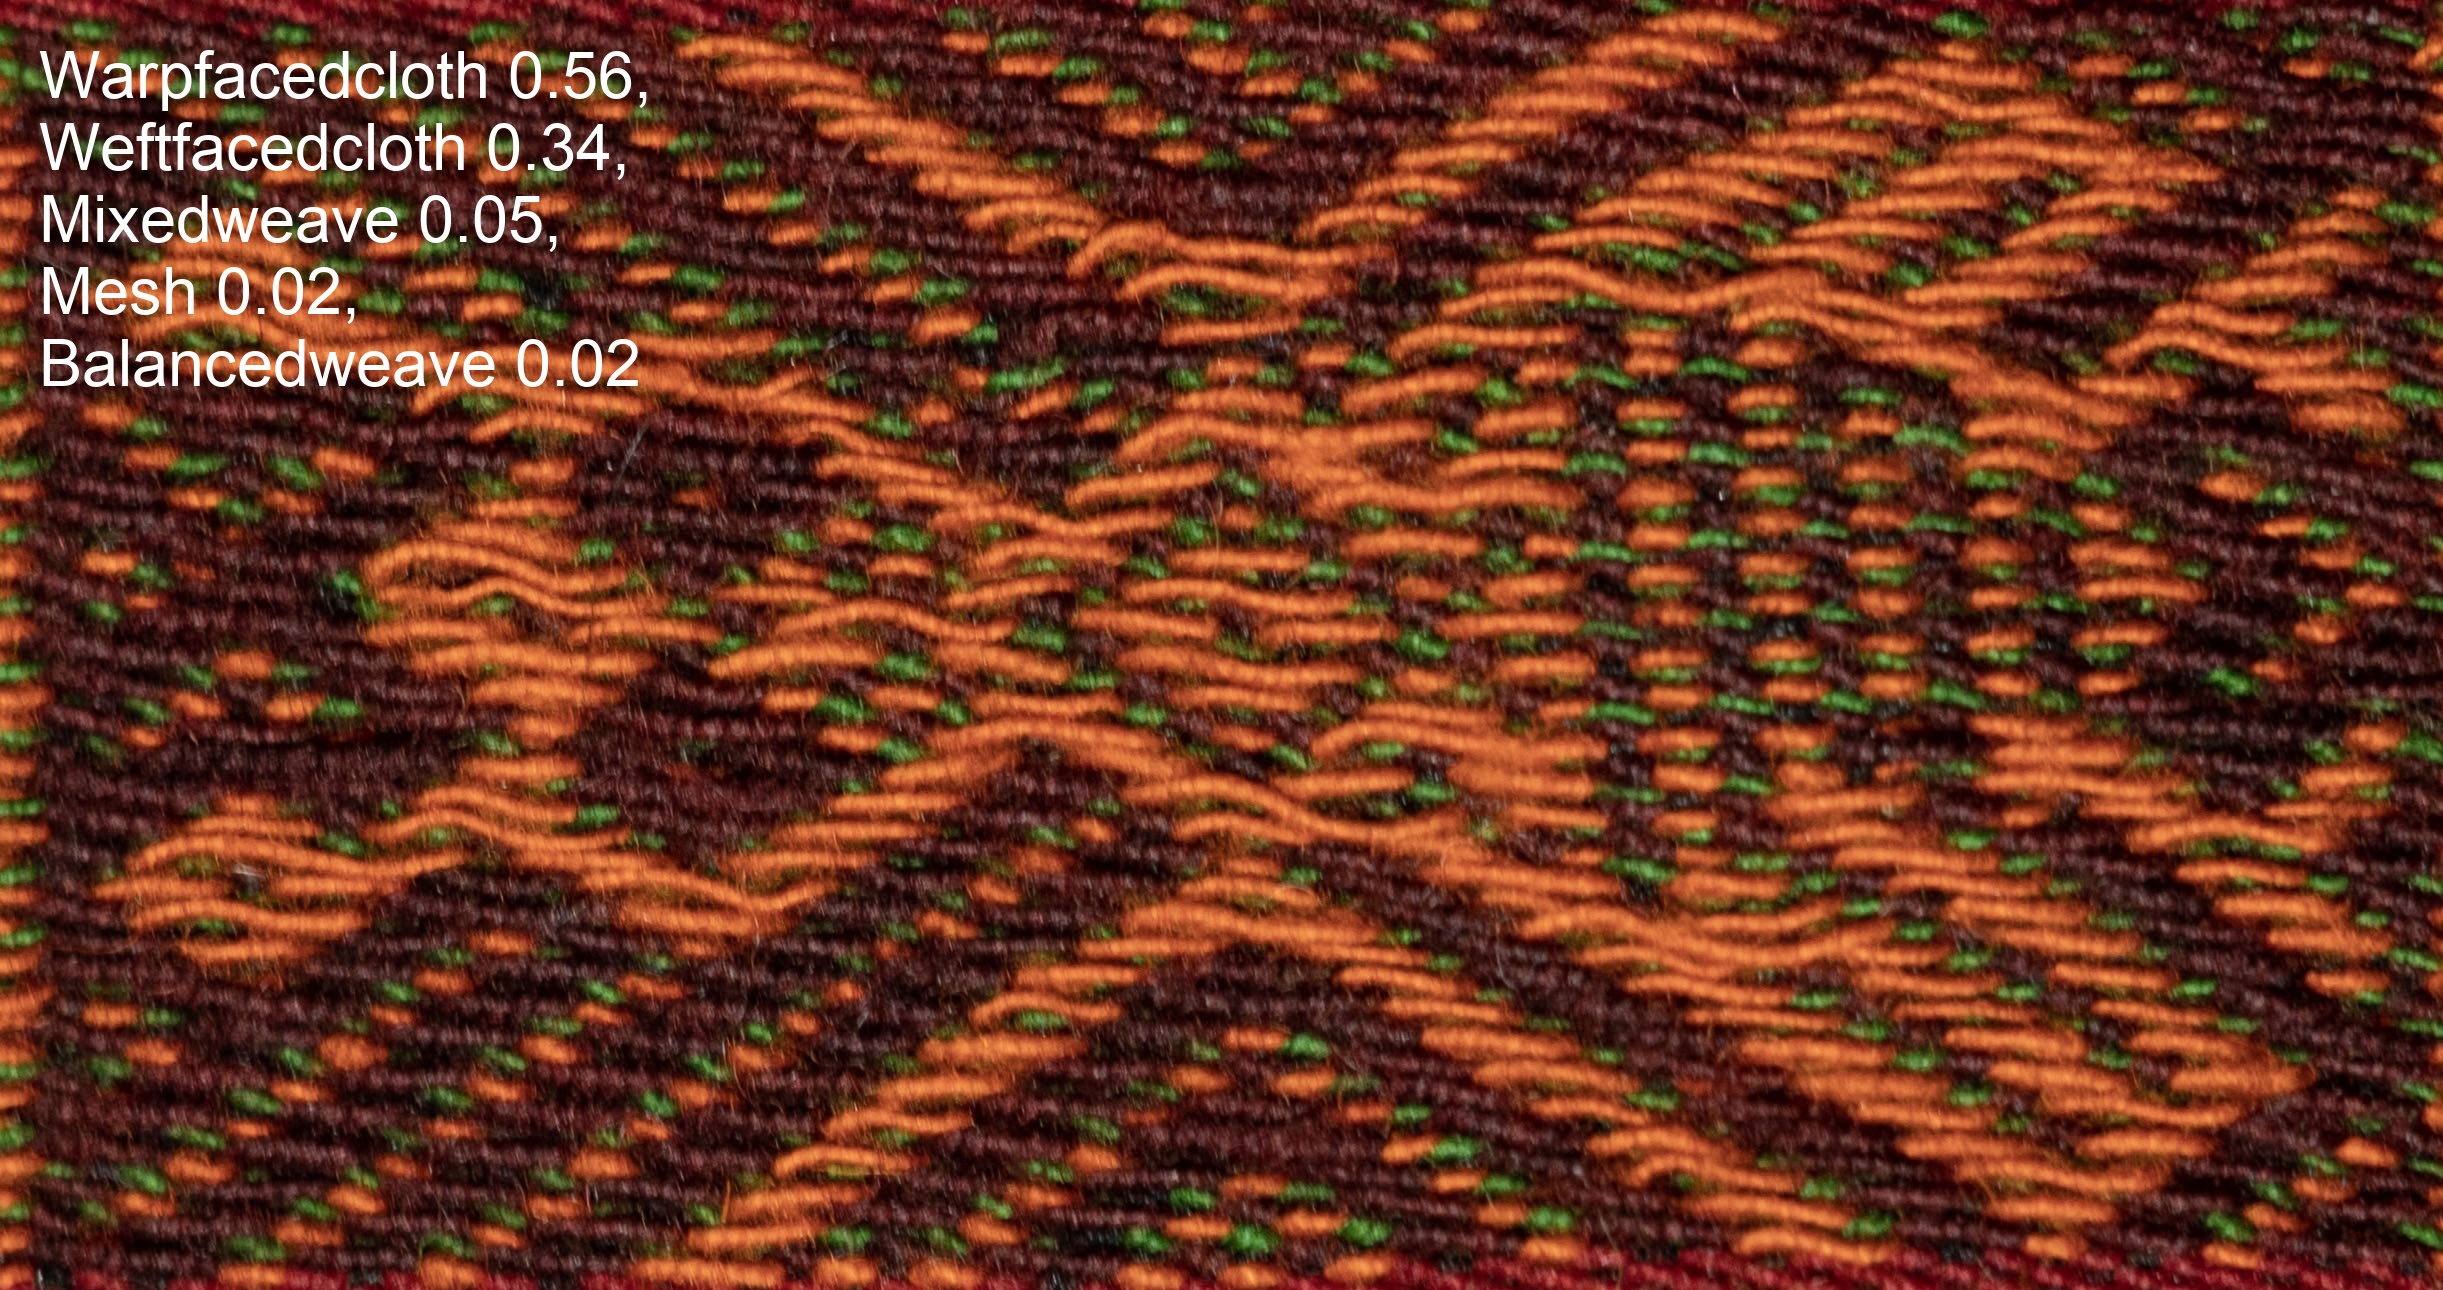
\includegraphics[height=5 cm]{../images/B2_Q10.jpg}
	\end{center}
    \end{minipage}
            \begin{minipage}[c]{.5\linewidth}
        \begin{center}
        		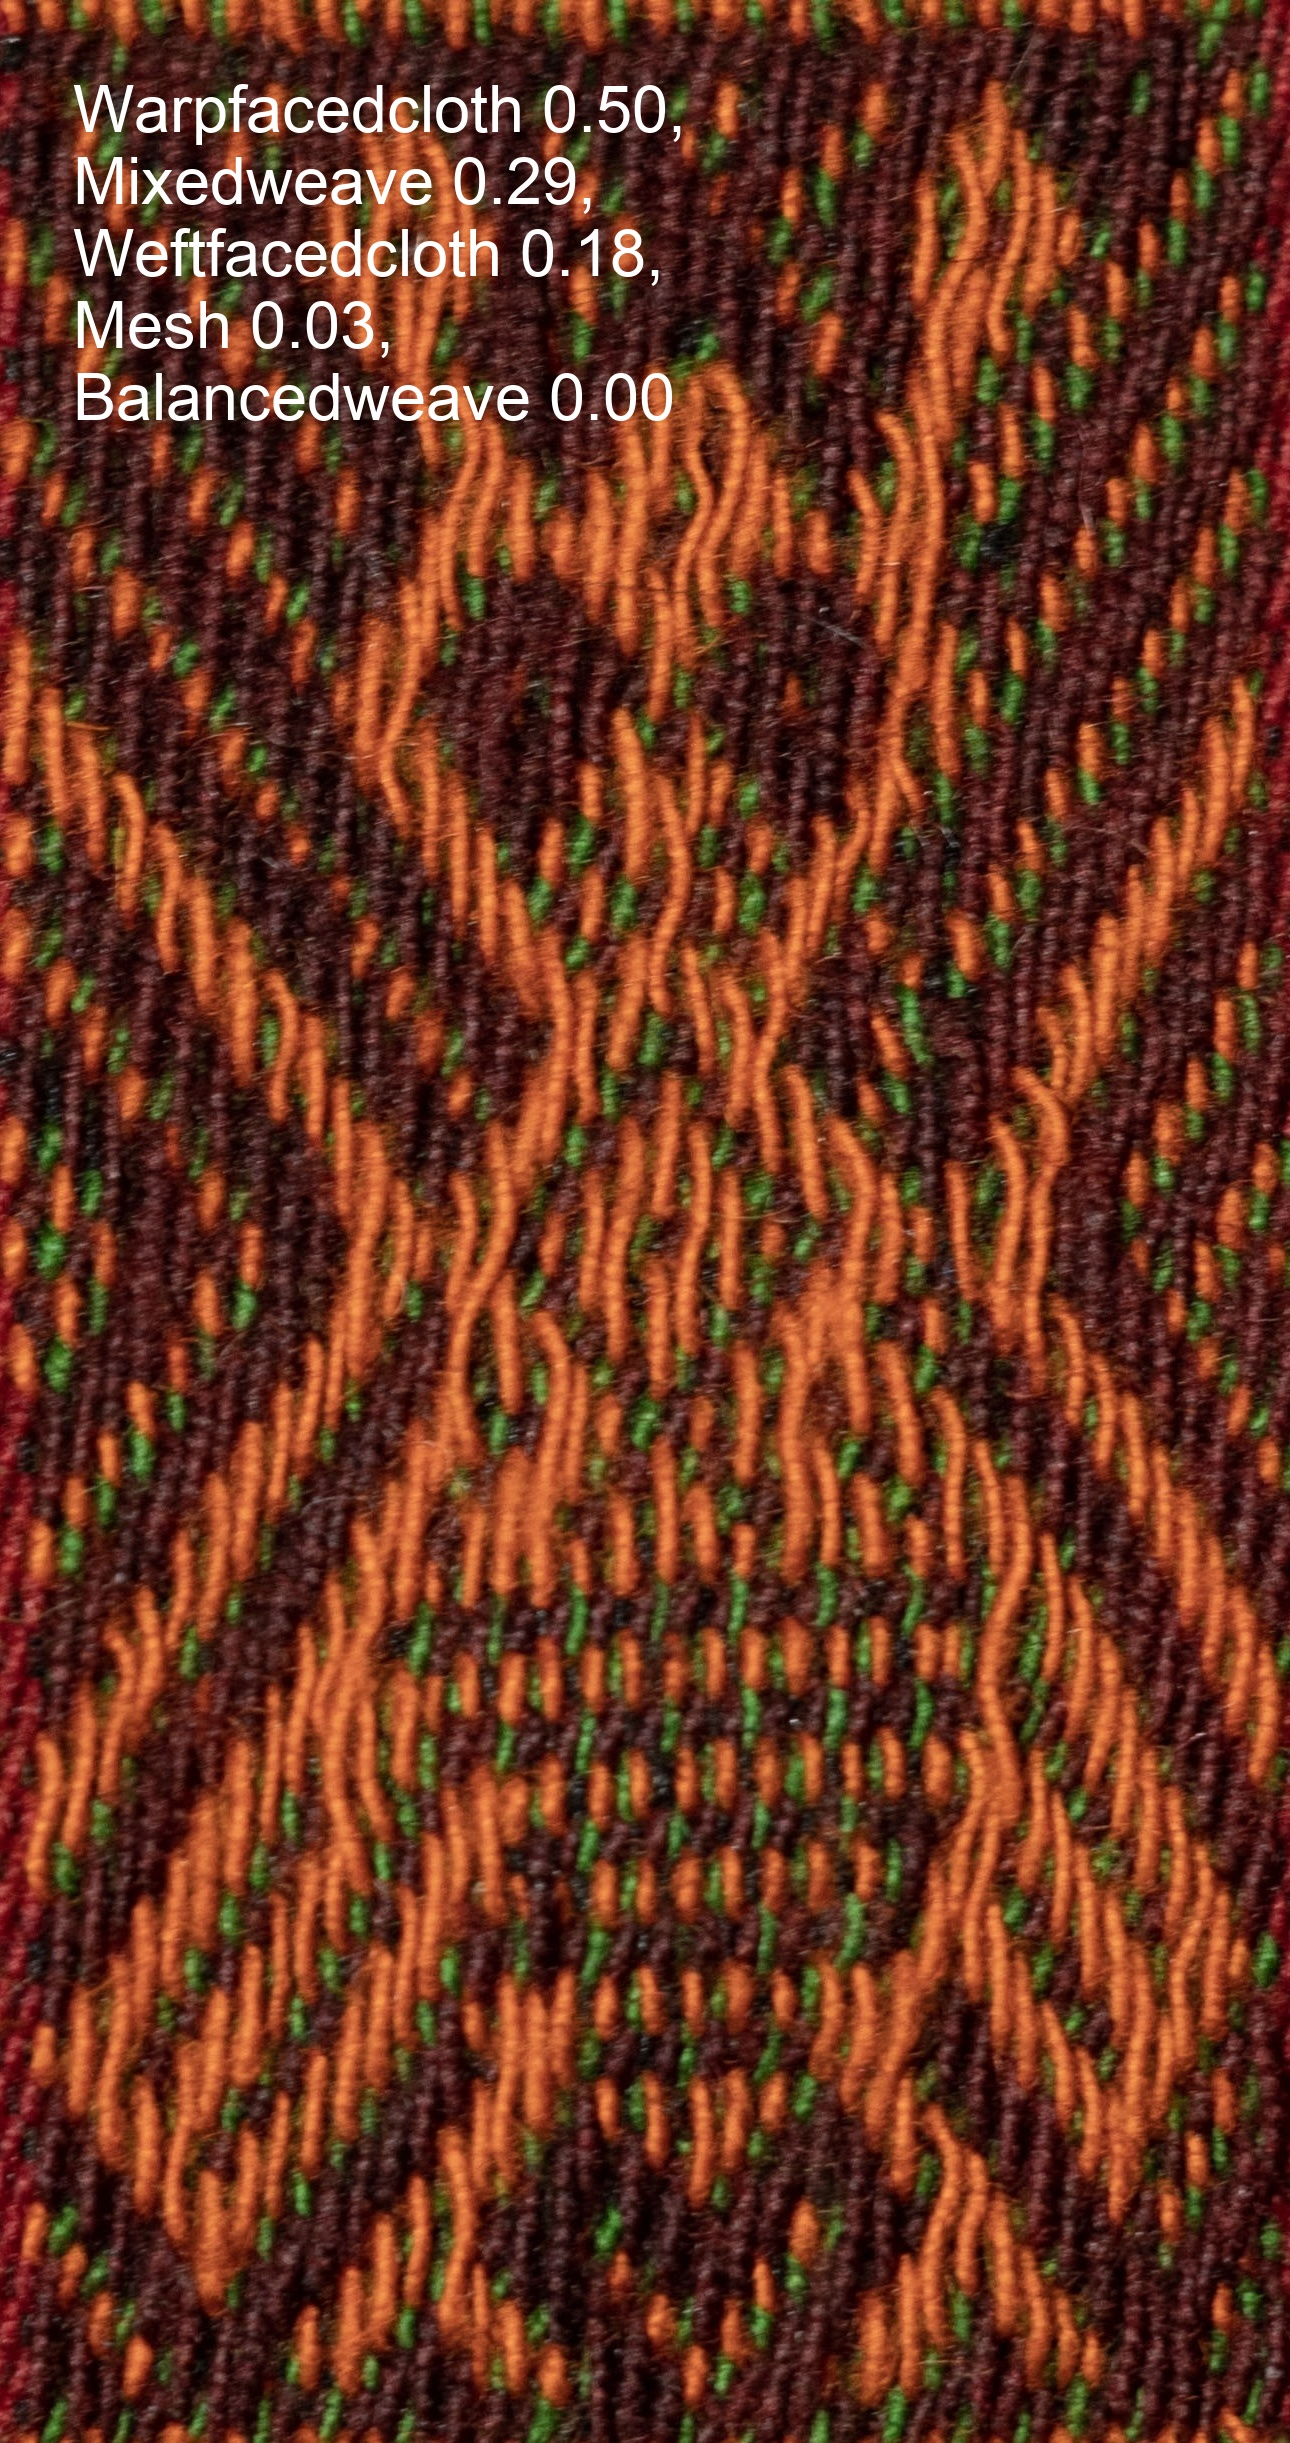
\includegraphics[height=7cm]{../images/B2_Q10r.jpg}
	\end{center}
    \end{minipage}
    \caption{Détail d'un tissage à dominante chaîne orienté différemment.}
\end{figure}

\subsubsection{Comparaison des résultats}

\begin{table}[!h]
    \centering
    \begin{tabular}{|c|c|}
        \hline
         \cellcolor{blue!20}\textbf{Organisation du dataset} & \cellcolor{blue!20}\textbf{\textit{Précision}}\\ \hline \hline
          Dataset initial & 92,4\% \\ \hline
          Dataset équilibré & 78,18\%  \\ \hline
          Dataset augmenté et équilibré & 90,78\% \\ \hline
    \end{tabular}
    \caption{Niveau de précision pour chaque modèle.}
    \label{tab:accuracy}
\end{table}

Nous obtenons la meilleure précision au cours du premier entraînement, sur le plus grand nombre d'images. Néanmoins, en équilibrant et augmentant le \textit{dataset} nous obtenons également une bonne précision globale et une meilleure précision par catégorie. Le niveau de précision obtenu est encourageant et semble indiquer qu'il est possible de détecter les techniques à partir des images des artefacts, première étape de compréhension des évolutions structurales des textiles andins. En comparaison, la méthode de classification des techniques proposée par l'équipe de SILKNOW utilisant un réseau de neurones convolutif avec une architecture ResNet obtenait une précision de 87,4\%\footcite[p.~53]{dorozynskiMultiTaskDeepLearning2019}.
Notre méthode mériterait donc d'être testée sur un \textit{dataset} plus large.




\section{Des sources iconographiques aux influences textiles}
\subsection{Observer les similarités textiles grâce à la classification non-supervisée ?}

La détection des techniques dans les textiles andins est certes une avancée par rapport à l'état de l'art actuel mais ne permet pas, en l'état, de saisir les influences et les hybridations techniques et stylistiques. Pour essayer de détecter les textiles détenant des traits iconographiques communs ou hybrides, nous devons essayer de rapprocher les images similaires. La similarité est une notion vague puisqu'elle indique ce \og qui est plus ou moins de même nature qu'une/que d'autre(s) entité(s); qui peut, sur certains points, être assimilé à une/à d'autre(s) entité(s)\fg\footnote{Source : CNRTL, \url{https://www.cnrtl.fr/definition/similaire}. Consulté le 27 mars 2024.}. Dans notre cas, il s'agit d'organiser les images de telle sorte que celles qui ont des éléments communs, techniques ou iconographiques, soient proches. Pour cela, nous allons également nous intéresser aux \textit{features} des images mais cette fois-ci en comparant directement leurs valeurs sans recourir à de l'annotation. Puisque les images ne sont pas annotées et que se sont seulement les valeurs des pixels qui sont prises en compte, il s'agit d'une classification non-supervisée des images\footcite[p.~439]{lecunDeepLearning2015}. Ce recoupement des images a lieu en plusieurs étapes : 
\begin{itemize}
	\item Récupération des \textit{features vectors} de chaque image.
	\item Projection des \textit{features vectors} dans un espace en deux dimensions.
	\item Récupération de \textit{clusters} d'images dont les \textit{features vectors} sont proches.\\
\end{itemize}

La récupération des caractéristiques discriminantes des images est réalisée par l'obtention de vecteurs représentant les valeurs de l'image. Ces \textit{features} servent de critères de comparaison. Pour cela, nous réutilisons le modèle YOLO, et ses résultats issus de la classification supervisée, auquel nous fournissons les poids de l'entraînement sur le corpus augmenté et équilibré\footnote{Nous avons également réalisé cette opération avec le modèle VGG16 pré-entraîné sur le \textit{dataset} d'ImageNet, soit près de 14 millions d'images labellisées et réparties en 1000 classes. Le code d'extraction de \textit{features} dans YOLO est extrait de \url{https://medium.com/@alaa99.awehbe/revolutionizing-analysis-feature-extraction-with-yolov8-revealed-0d4ab4a56e26} et \url{https://github.com/ultralytics/ultralytics/issues/1724}.}. Nous utilisons ces poids puisque nous savons qu'ils rapprochent les images qui ont des caractéristiques techniques similaires. Les vecteurs utilisés sont extraits de la dernière couche convolutive du réseau (voir \ref{fig:YOLO}). Cette méthode est appelée apprentissage par transfert puisque nous utilisons un modèle déjà pré-entraîné pour extraire les \textit{features} de chaque image\footcite[p.~3]{hosnaTransferLearningFriendly2022}.
Nous pouvons déjà souligner un biais : les images fournies au modèle ont servi à l'apprentissage du modèle et seront donc correctement classifiées. Toutefois, puisque nous ne sommes pas dans un processus de classification mais dans un processus de recherche de similarité,  cela nous indique que les \textit{features} des images d'entraînement appartenant à la même classe seront probablement proches. \\

\begin{figure}[!h]
	\begin{center}
		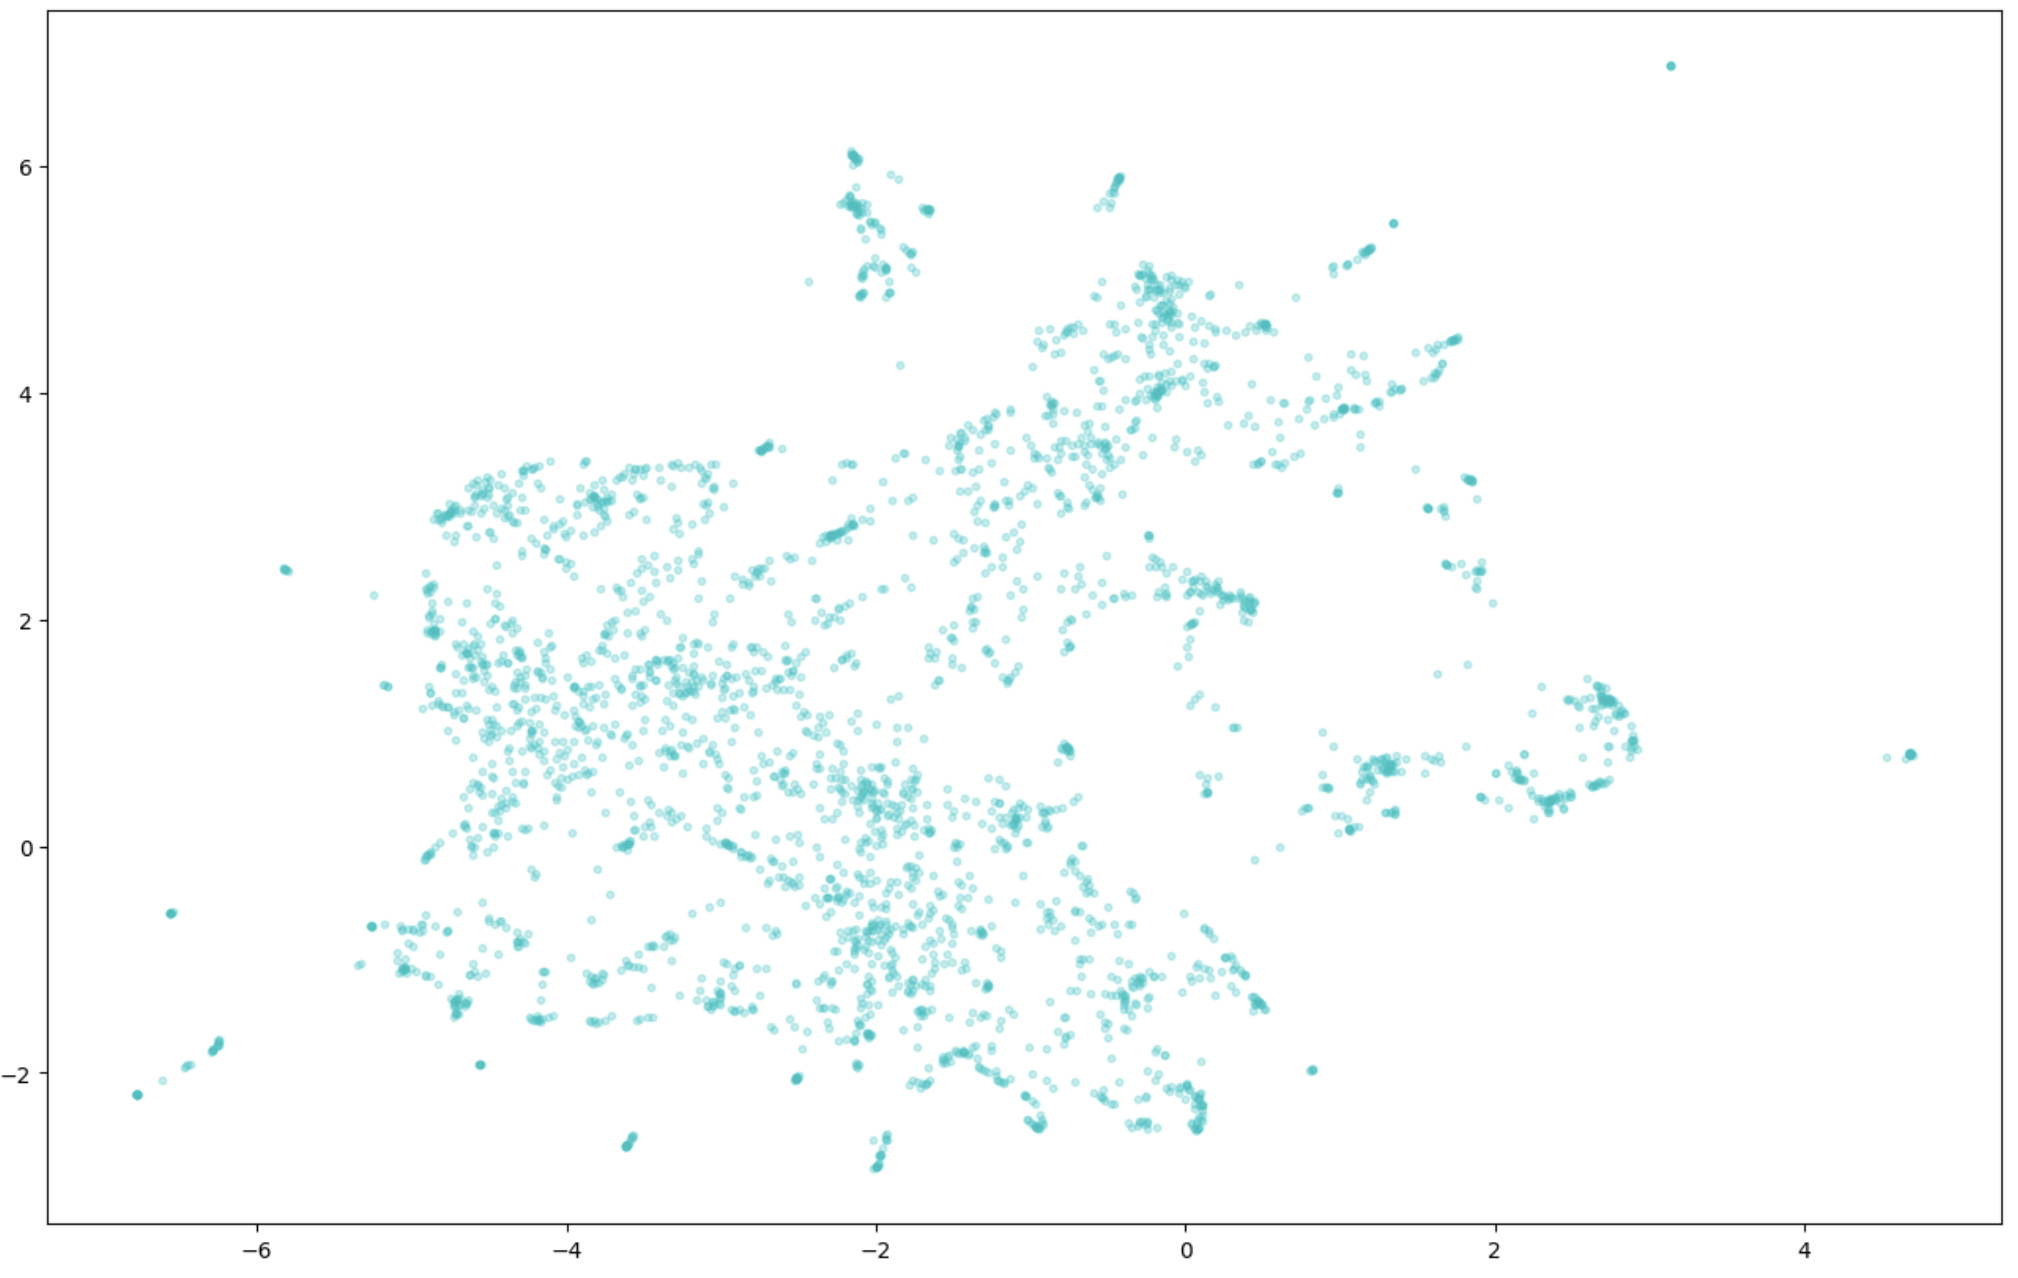
\includegraphics[width=16cm]{../images/YOLO_NS_UMAP.png}
		\caption{Projection des vecteurs dans un espace en deux dimensions (algorithme UMAP). \\ Paramètres : n\_neighbors=10, min\_dist=0.0,  n\_components=2.}
	 \end{center}
\end{figure}

Les \textit{features vectors} sont des tenseurs (tableaux multidirectionels) de dimension (1, 256, 7, 7).
Pour travailler à partir de ces vecteurs, nous utilisons un algorithme de réduction de dimension qui nous permet de les visualiser dans un espace en deux dimensions. Nous avons utilisé l'algorithme \textit{Uniform Manifold Approximation and Projection} (UMAP) pour ce faire\footnote{L'analyse en composantes principales (PCA), autre méthode de réduction de dimension, ne s'est pas avérée efficace pour représenter les données de manière discriminante.}. Il s'agit d'un algorithme topologique dont le but premier est de garder l'organisation topologique des données\footcite[p.~13]{mcinnesUMAPUniformManifold2018}, c'est-à-dire de garder les structures locales et globales des données. Les paramètres de l'algorithme permettent d'ailleurs de déterminer si l'on favorise les structures locales, en diminuant le nombre de voisins de chaque élément, ou la vision globale, en diminuant la distance entre éléments. En réduisant la distance minimale entre éléments, nous favorisons l'agglomération des \textit{features} afin d'obtenir des \textit{clusters} distincts.

Après avoir obtenu une représentation des \textit{features vectors} en deux dimensions, nous pouvons réaliser un \textit{clustering}, c'est-à-dire une partition des données en sous-groupes ou \textit{clusters}. Selon la méthode utilisée, les éléments représentés ne seront pas regroupés de la même manière. Nous avons testé deux méthodes de \textit{clustering} : 
\begin{itemize}
	\item Méthode des \textit{k}-moyens\footnote{Voir la documentation : \url{https://scikit-learn.org/stable/modules/generated/sklearn.cluster.KMeans.html}, consultée le 26 mai 2024.} : il s'agit d'une méthode de partition des données en un nombre \textit{k} défini de sous-groupes, selon une mesure de distance spécifiée. Chaque élément est associé à un seul des \textit{k} groupes par un identifiant numérique.
	\item Méthode HDBSCAN\footnote{Voir la documentation : \url{https://hdbscan.readthedocs.io/en/latest/parameter_selection.html}, consultée le 26 mai 2024 ainsi que l'article \cite{mcinnesHdbscanHierarchicalDensity2017}.} : méthode de partition des données qui ne nécessite pas de nombre défini d'agrégats voulus. Les données sont organisées selon un nombre de paramètres : 
	\begin{itemize}
		\item \textbf{min\_cluster\_size} : choix du plus petit nombre d'éléments que l'on considère comme composant un \textit{cluster}.
		\item \textbf{max\_cluster\_size} : choix du plus grand nombre d'éléments que l'on considère comme composant un \textit{cluster}.
		\item \textbf{min\_samples} : distingue le bruit des éléments des \textit{clusters} (zone les plus denses). En l'augmentant, on augmente ce qui est considéré comme bruit. Par défaut, il prend la même valeur que \textbf{min\_cluster\_samples}, le réduire permet de garder plus de \textit{clusters} différents.
		\item \textbf{cluster\_selection\_epsilon} : conserve des grands \textit{clusters} dans les zones les plus denses (même si \textbf{min\_cluster\_size} est faible)
	\end{itemize}
Cet algorithme tient compte du bruit c'est-à-dire qu'il ne prend pas en compte le éléments les plus dispersés, ceux qu'il n'arrive pas à attribuer à un \textit{cluster}. Dans cette configuration, certains éléments n'appartiennent donc à aucun \textit{cluster}. \\
\end{itemize}

\begin{figure}[!h]
	\begin{center}
		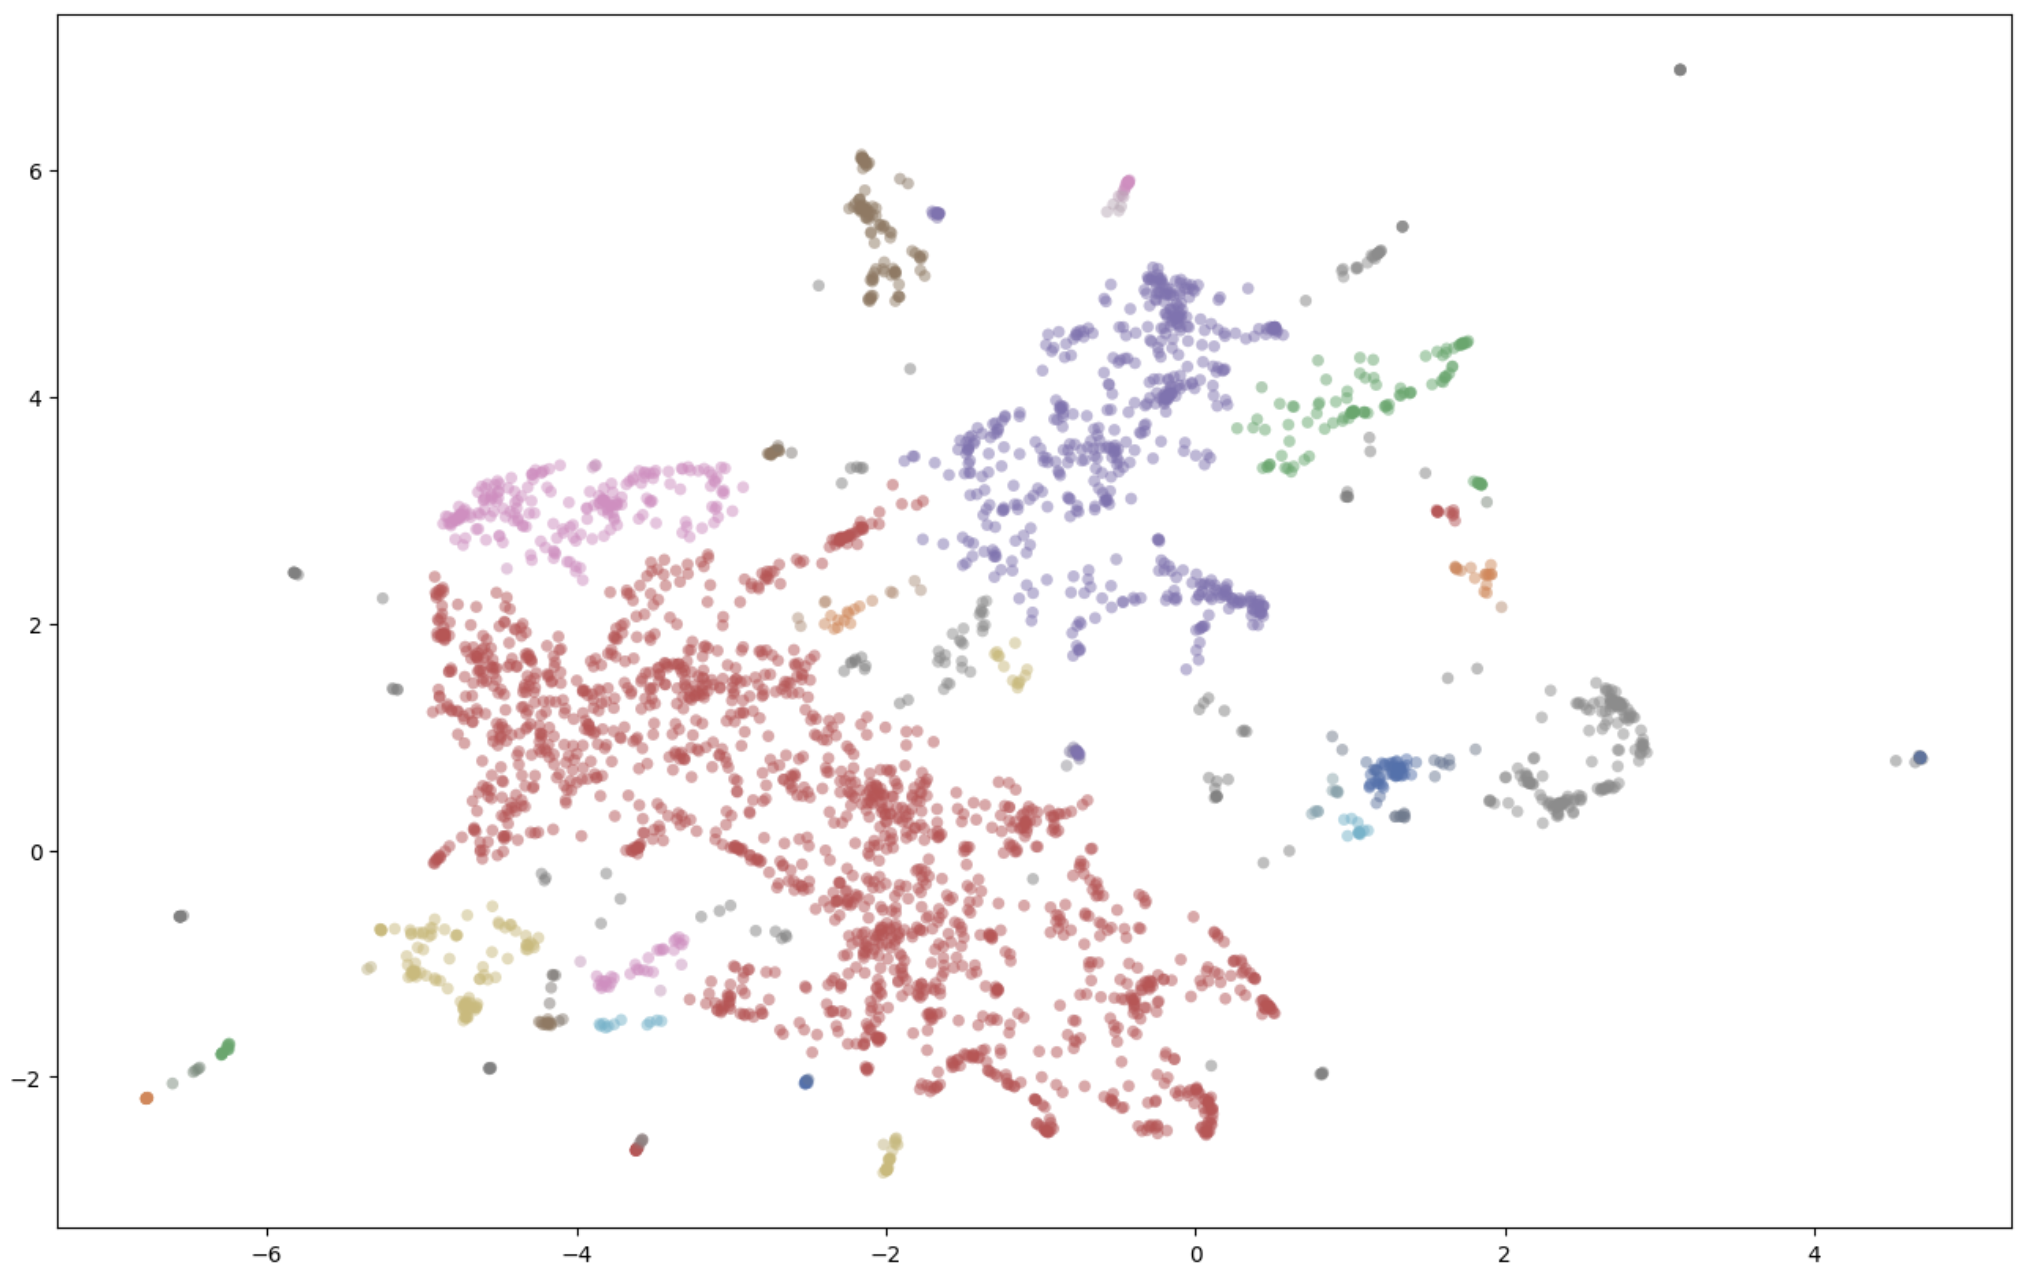
\includegraphics[width=16cm]{../images/YOLO_NS_HDBSCAN.png}
		\caption{\textit{Clustering} HDBSCAN des \textit{features} des images. \\ Paramètres :  min\_cluster\_size=10, min\_samples=1, cluster\_selection\_epsilon=0.2.}
	 \end{center}
\end{figure}

\noindent Avec la partition HDBSCAN, nous récupérons trois grands clusters, composés de 1583 images (en rouge), 517 images (en violet) et de 205 images (en rose). Le reste des \textit{clusters} sont composés de peu d'images (entre 10 et 30). Une bonne partie de ces petits clusters est uniquement composée de photographies de maquettes (voir les exemples de maquettes, page \pageref{fig:MEE004B}), le reste des textiles est concentré dans les grands \textit{clusters}. Par ailleurs, l'organisation des \textit{features} repose en grande partie sur la composition des images, plus que sur les éléments des textiles. Ainsi, le \textit{cluster} 24 (en violet) est composé de bandes de textiles verticales entourées de fond blanc. En outre, une partie des points n'est pas attribuée à un \textit{cluster} (en gris sur le graphique). C'est pourquoi nous avons favorisé l'algorithme des \textit{k}-moyens qui génère une partition de la partie centrale du graphique et qui prend en compte la totalité des points.

\begin{figure}[!h]
	\begin{center}
		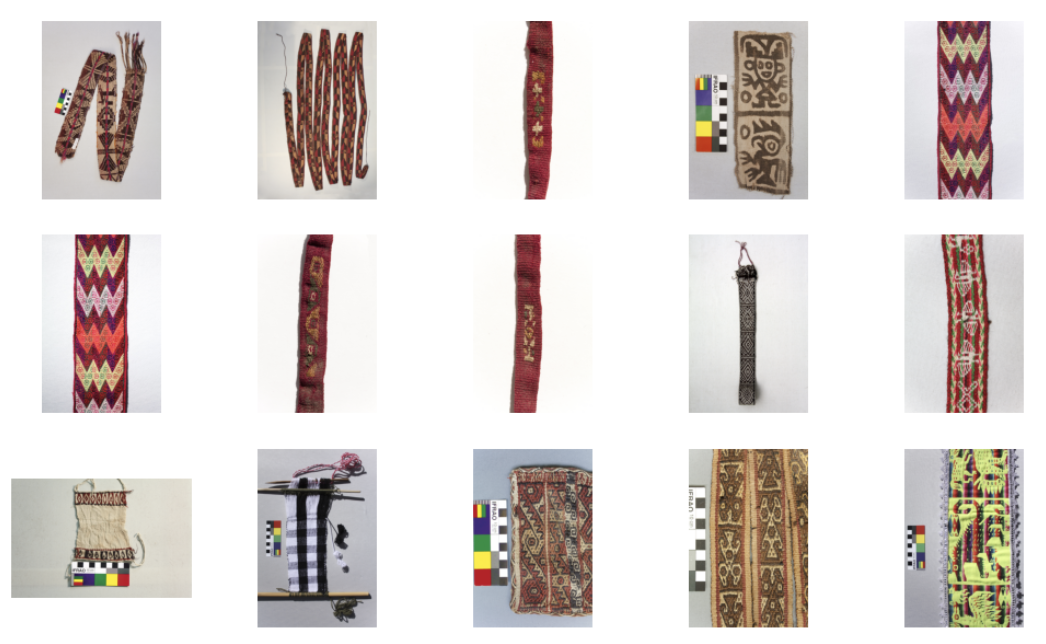
\includegraphics[width=12cm]{../images/YOLO_NS_HDBSCAN_24.png}
		\caption{\textit{Cluster} numéro 24 de la partition HDBSCAN}
	 \end{center}
\end{figure}

Nous avons utilisé la partition HDBSCAN comme référence du nombre de \textit{clusters} à obtenir avec l'algorithme des \textit{k}-moyens, auquel nous avons donc demandé 30 \textit{clusters}. Ces derniers restent de grande taille puisqu'il s'agit de classer 3301 images en 30 \textit{clusters}.

\subsection{Saisir les imitations et les ré-interprétations textiles à partir du \textit{clustering} des \textit{features} des images}

\begin{figure}[!h]
	\begin{center}
		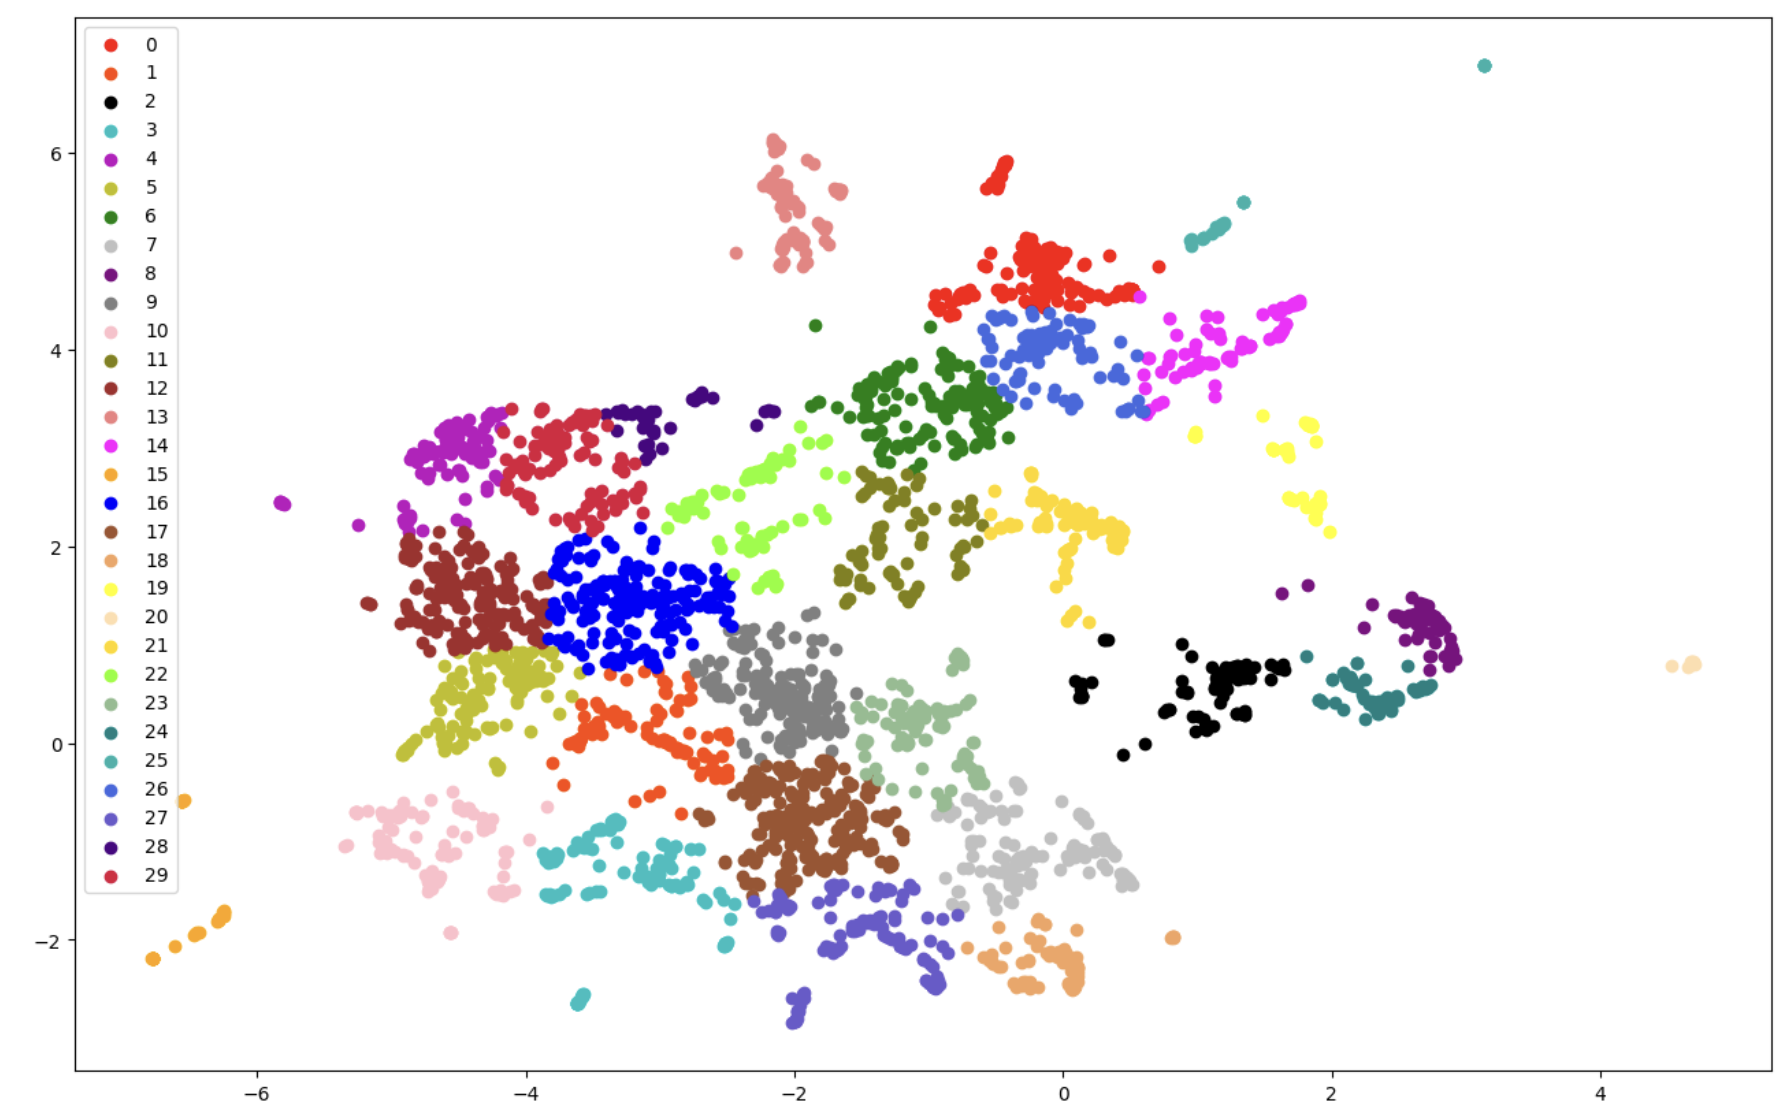
\includegraphics[width=16cm]{../images/YOLO_NS_KMEAN.png}
		\caption{\textit{Clustering} KMEANS des \textit{features} des images \\ Paramètre : n\_clusters=30}
	 \end{center}
\end{figure}

Nous allons donc analyser les résultats de l'extraction de \textit{features}, avec une réduction de dimension UMAP et un \textit{clustering k}-moyens.
Là encore les  \textit{clusters} semblent être largement déterminés par la prise de vue de l'image. Ainsi, le \textit{cluster} 21 (en jaune foncé) est composé de bandes verticales accompagnées d'une règle IFRAO sur leur gauche. Les \textit{clusters} 6 et 26 sont déterminés par des textiles entourés d'un fond blanc et les \textit{clusters} 0, 2, 8, 14, 19, 20, 24 et 25 (à l'extrême droite du graphique) regroupent uniquement des maquettes. Les \textit{clusters} ainsi composés ne sont pas incohérents mais ne permettent pas d'obtenir d'informations probantes. 

Puisque le corpus détient en moyenne 5 images par textile, un textile peut se trouver dans plusieurs \textit{clusters}, notamment dans les \textit{clusters} composés d'images de détails des textiles. C'est un avantage puisque selon les parties du textile étudiées, les \textit{features} pourrons effectuer des rapprochements avec une plus grande variété de textiles. Les \textit{clusters} composant le bas du graphique semblent ainsi se distinguer par des caractéristiques iconographiques. Par exemple, le \textit{cluster} 4 regroupe des \textit{mantas} républicaines et coloniales, malgré les prises de vue diverses. Nous retrouvons dans ce cluster la \textit{manta} coloniale présentée dans le premier chapitre (voir \ref{fig:MSF102}) qui, nonobstant sa réalisation en tapisserie (face trame), est réunie avec des \textit{mantas} en tissage face chaîne. Le critère de similarité iconographique semble déterminant dans ce cas. Il est d'ailleurs intéressant de voir qu'elle est majoritairement associée à des textiles républicains et non à des textiles pré-hispaniques dont on aurait pu imaginer qu'elle reprenait certains traits. Le \textit{cluster} voisin, 12, contient également des détails de \textit{mantas} alternant bandes unies et fines lignes de motifs. Elles sont tout à fait distinctes des \textit{clusters} de \textit{mantas} 5 et 10 (en dessous sur le graphique) structurés autour de textiles avec des bandes larges de \textit{pallay}, motifs tissés. Ces quatre \textit{clusters} de \textit{mantas} sont principalement composés de tissages républicains des hautes-terres. Les textiles côtiers à dominante chaîne plus anciens que l'on trouve dans ces \textit{clusters} n'ont pas de traits iconographiques qui permettraient de les lier avec certitude aux textiles des hautes-terres.


%\begin{figure}[!h]
%	\begin{center}
%		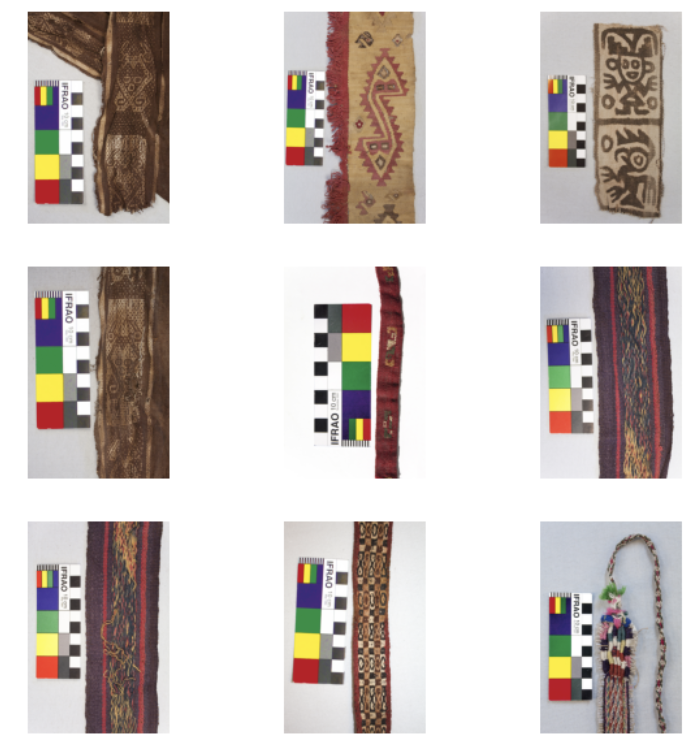
\includegraphics[height=7cm]{../images/YOLO_NS_KMEAN_21.png}
%		\caption{Images extraites du \textit{cluster} 21 (jaune foncé).}
%	 \end{center}
%\end{figure}
%
%\begin{figure}[!h]
%	\begin{center}
%		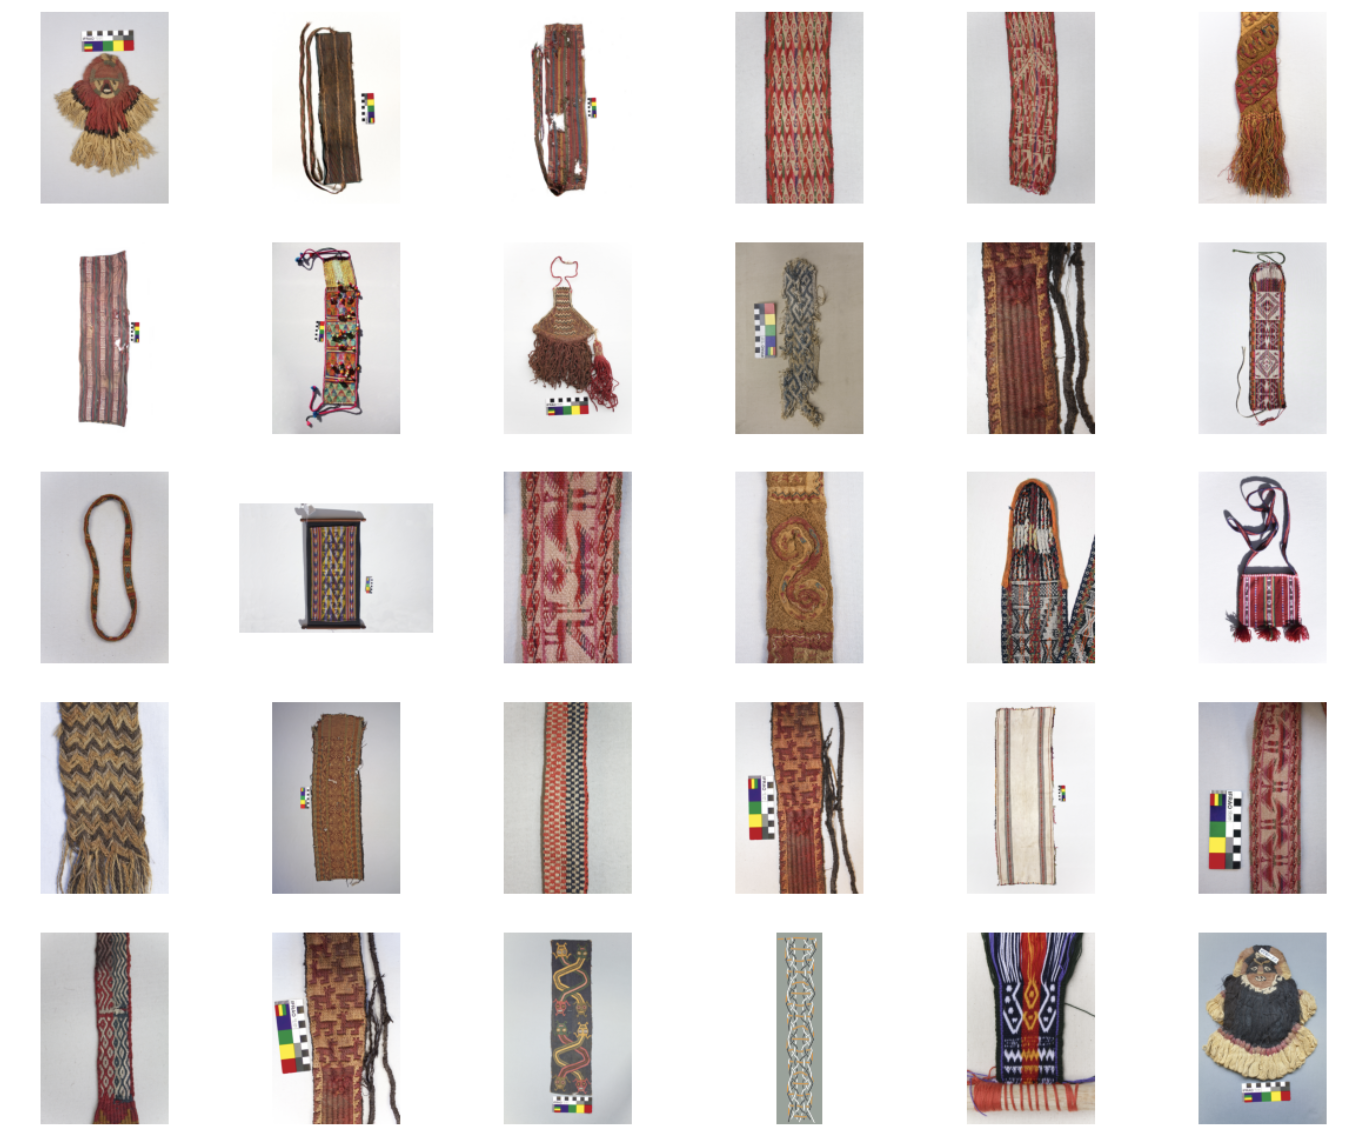
\includegraphics[height=7cm]{../images/YOLO_NS_KMEAN_6.png}
%		 \caption{Images extraites du \textit{cluster} 6 (vert foncé).}
%	 \end{center}
%\end{figure}

\begin{figure}[!h]
\begin{minipage}[c]{.5\linewidth}
      \begin{center}
       		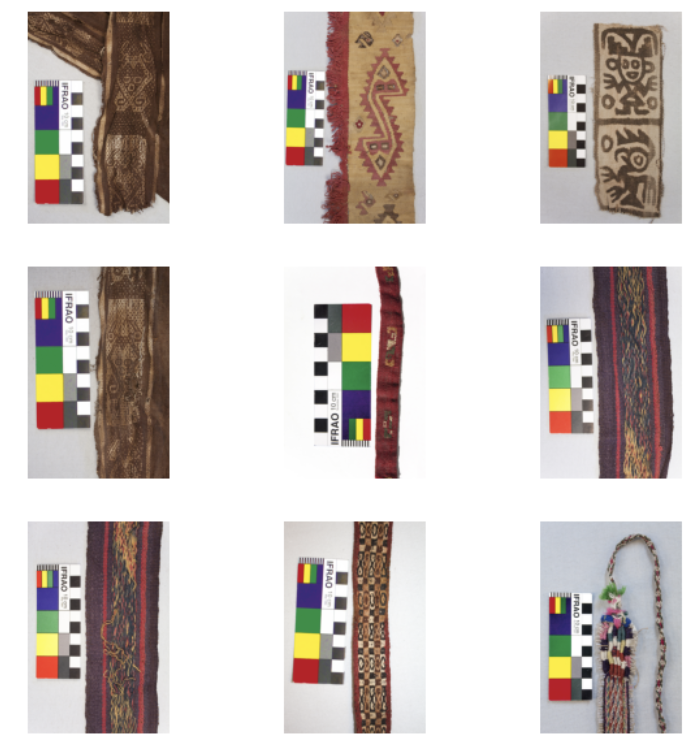
\includegraphics[height=7cm]{../images/YOLO_NS_KMEAN_21.png}
		 \caption{Images extraites du \textit{cluster} 21 (jaune foncé).}
		 \label{fig:c21}
	\end{center}
    \end{minipage}
    \hspace{5pt}
    \begin{minipage}[c]{.5\linewidth}
        \begin{center}
        		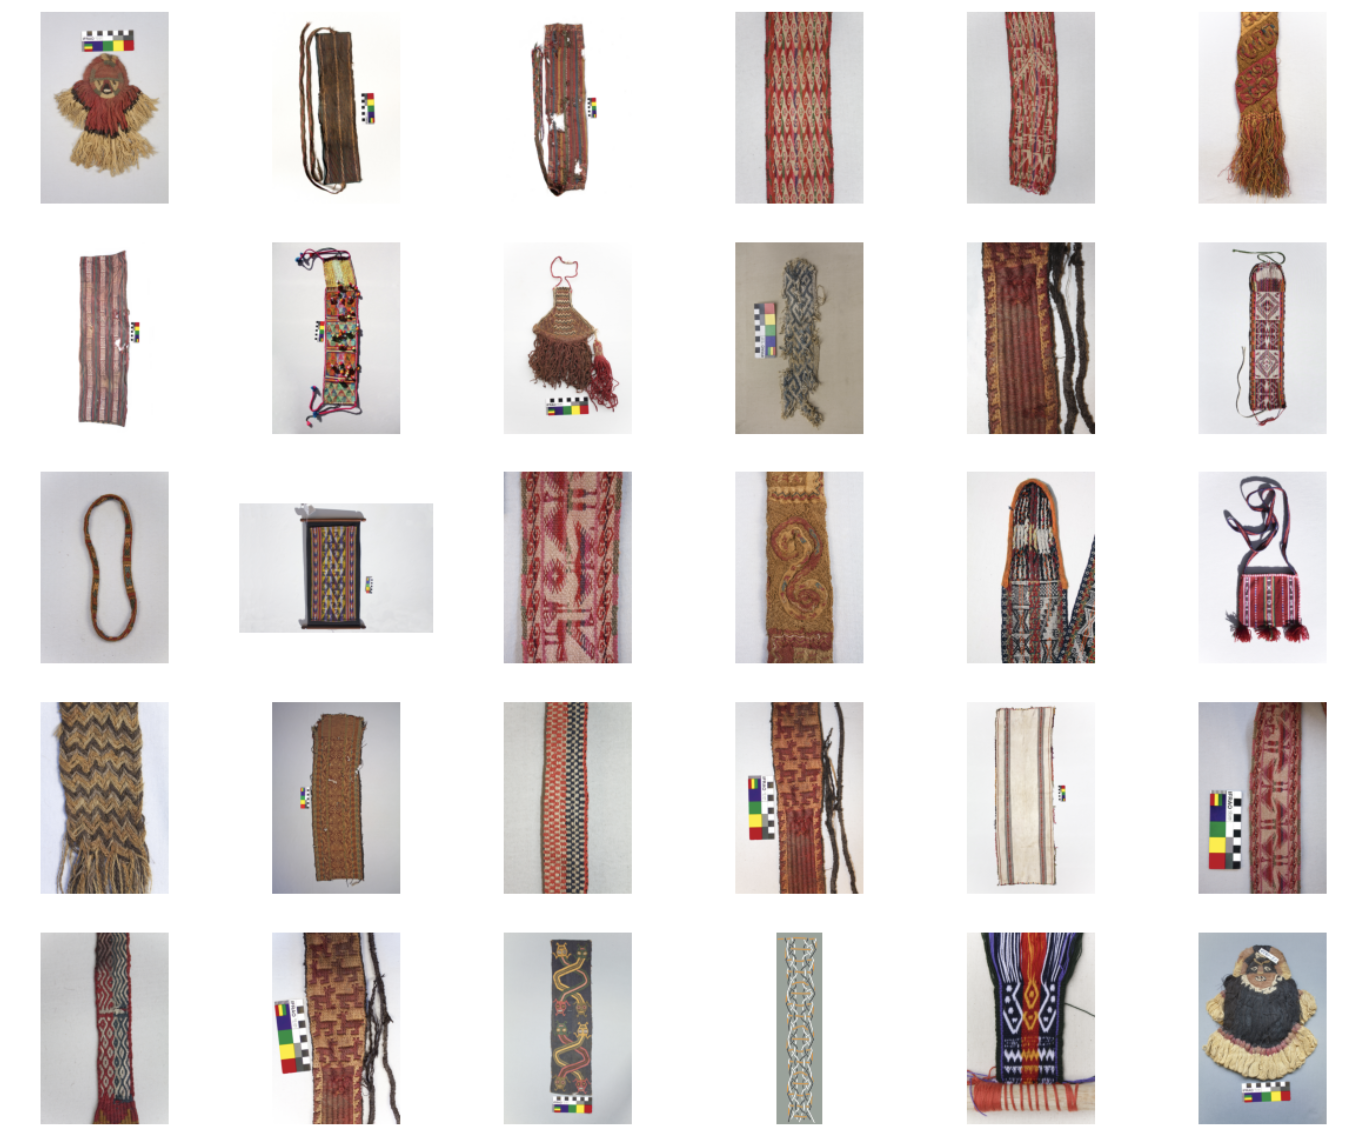
\includegraphics[height=7cm]{../images/YOLO_NS_KMEAN_6.png}
		 \caption{Images extraites du \textit{cluster} 6 (vert foncé).}
		 \label{fig:c6}
	\end{center}
    \end{minipage}
\end{figure}

\begin{figure}[!h]
 \begin{minipage}[c]{.5\linewidth}
        \begin{center}
        		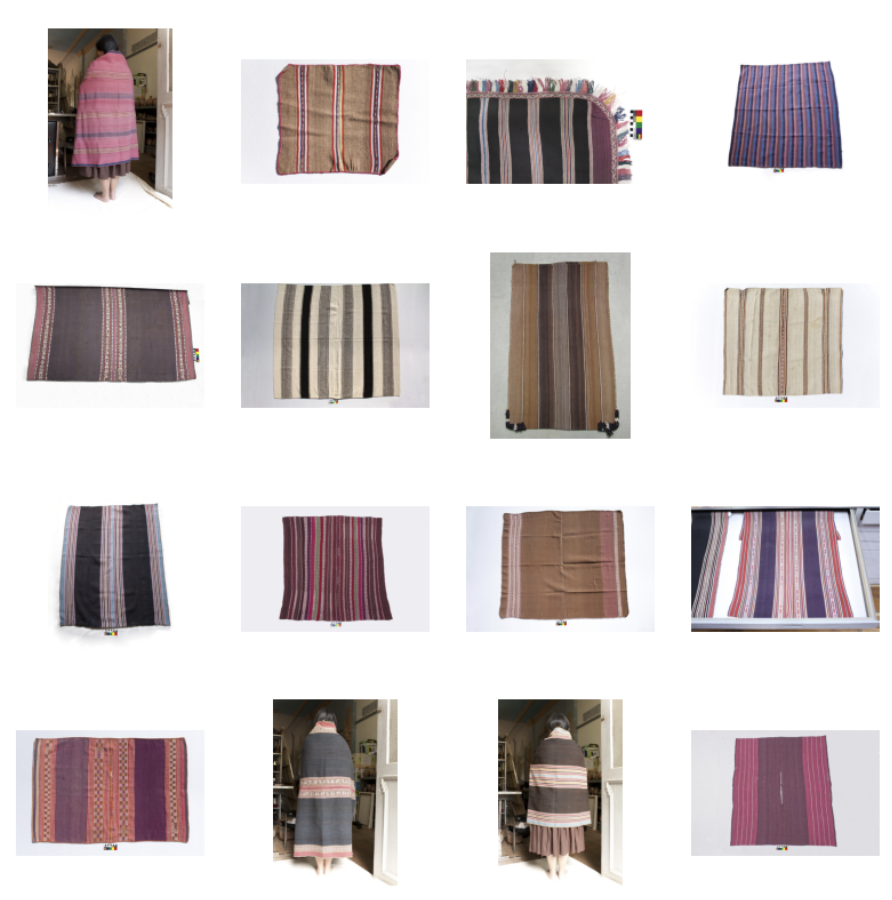
\includegraphics[width=8cm]{../images/YOLO_NS_KMEAN_4.png}
		\caption{Images extraites du \textit{cluster} 4 (fuchsia).}
		\label{fig:c4}
	\end{center}
    \end{minipage}
    \hspace{5pt}
    \begin{minipage}[c]{.5\linewidth}
        \begin{center}
        		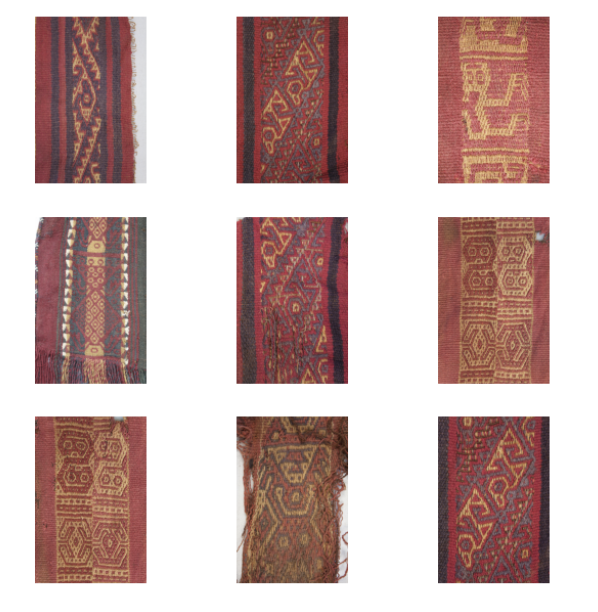
\includegraphics[width=8cm]{../images/YOLO_NS_KMEAN_3.png}
		\caption{Images extraites du \textit{cluster} 3 (bleu clair).}
		\label{fig:c3}
	\end{center}
    \end{minipage}
\end{figure}

De la même manière, le \textit{cluster} 3 concentre les motifs côtiers en tissage à dominante trame et en tissage à dominante chaîne. En son sein, apparaissent des rapprochements iconographiques entre techniques mais également entre lieux de production et entre collections muséales, comme nous pouvons le voir à partir des deux images suivantes extraites du \textit{cluster}. Ces deux exemples sont à rapprocher du tissage à dominante chaîne présenté dans le premier chapitre, provenant d'Ica, sur la côte sud du Pérou à la même période qui se trouve également dans ce \textit{cluster} (voir textile BML019, page \pageref{fig:BML019}). Ces trois textiles portent les traits caractéristiques présentés par Sophie Desrosiers comme preuves d'un transfert technique et iconographique au cours de la période Intermédiaire Tardive : délimitation des motifs en noir, points alternés sur toute la bande et formes triangulaires\footcite[p.~5]{desrosiersRevisitingOcucajeOpened2008}. Dans notre base de données, nous n'avons pas de traces de circulations entre la société Chancay et la société Ica, sociétés qui occupaient le territoire côtier à la même période, sans être voisines. Ces textiles pourraient alors être des indices d'une influence commune venue des hautes-terres, adaptée aux techniques textiles maîtrisées par les civilisations côtières.

\begin{figure}[!h]
 \begin{minipage}[c]{.5\linewidth}
        \begin{center}
        		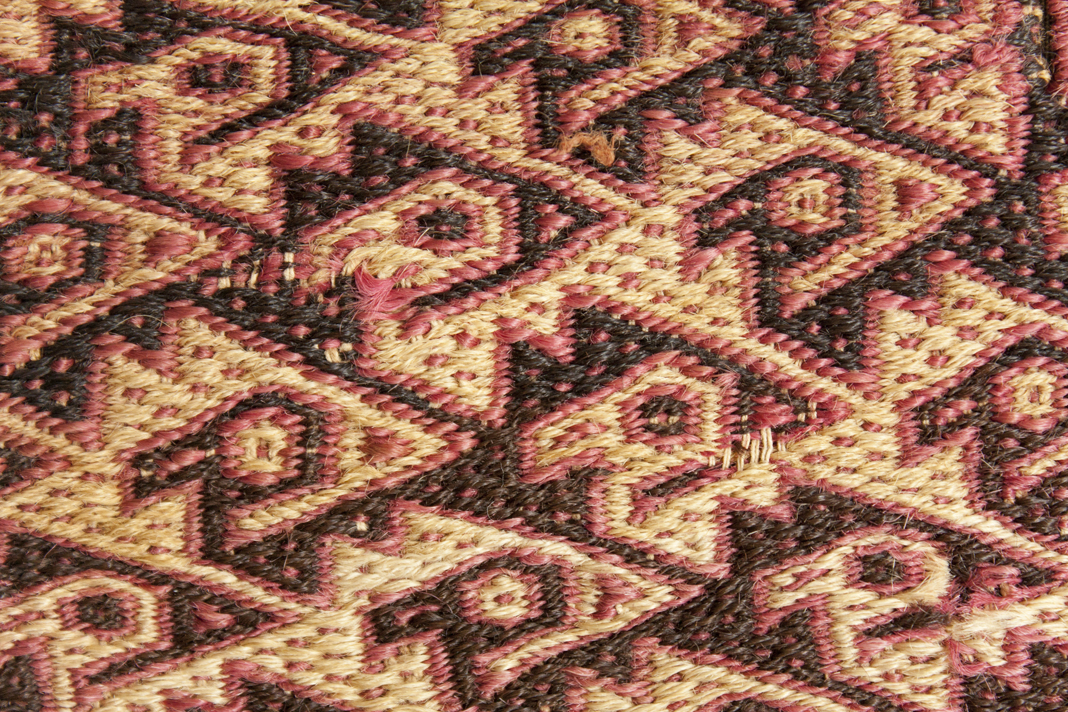
\includegraphics[width=6cm]{../images/VAM009.jpg}
		\caption{Tissage à dominante trame, provenant de Chancay (côte centrale du Pérou), période Intermédiaire Tardive. \\ Référence dans la base de données : VAM009.}
		\label{fig:VAM009}
	\end{center}
    \end{minipage}
    \hspace{5pt}
    \begin{minipage}[c]{.5\linewidth}
        \begin{center}
        		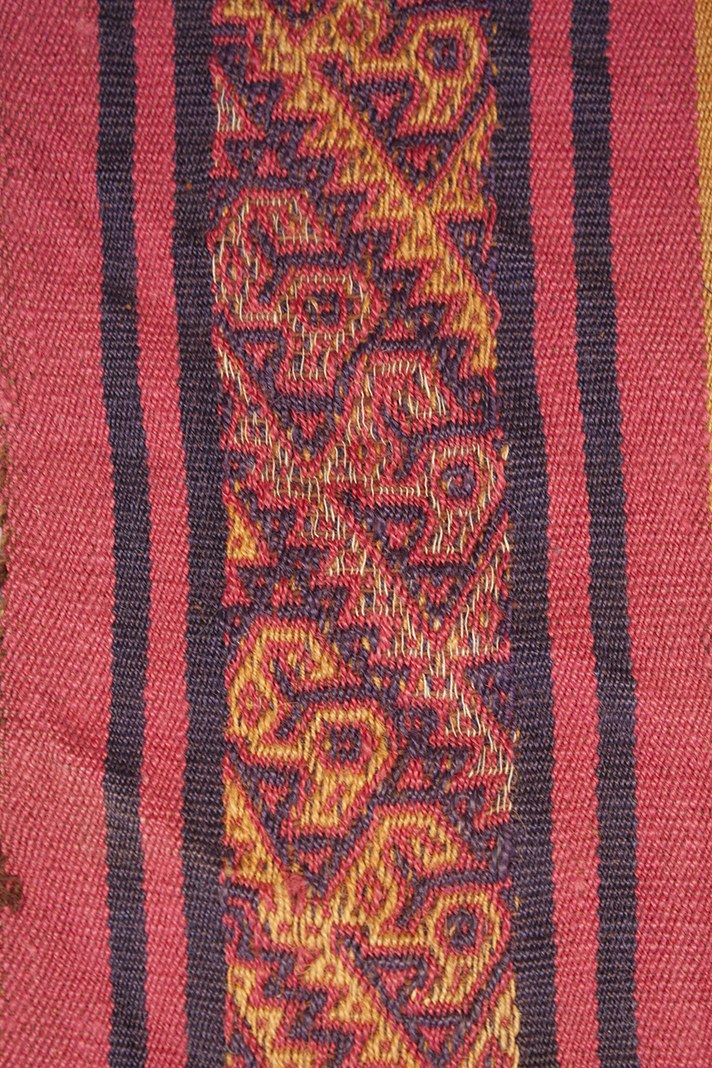
\includegraphics[height=6cm]{../images/BML032.jpg}
		\caption{Tissage à dominante chaîne, provenant de Chancay (côte centrale du Pérou), période Intermédiaire Tardive. \\ Référence dans la base de données : BML032.}
		\label{fig:BML032}
	\end{center}
    \end{minipage}
\end{figure}

Le \textit{cluster} 7 regroupe également des textiles côtiers aux traits iconographiques similaires. Le motif à têtes d'oiseaux que nous pouvons observer sur les tissages ci-dessous est présent dans 15 images de ce \textit{cluster}. Sa présence atteste d'une iconographie commune partagée, au moins, par les civilisations côtières de l'Intermédiaire Tardif : Chancay, Ica et Chimú. Le regroupement de textiles Chancay et Chimú est intéressante puisque nous avons, dans notre base  de données, des traces d'échanges entre ces civilisations ainsi que le partage de traits communs, avec l'analyse des poupées inhumées. Dans ce même \textit{cluster}, on retrouve le textile brodé de l'Intermédiaire Ancien (voir \ref{fig:VAM005}), indice d'une perdurance de ce motif dans les broderies sur le long terme sur la côte centrale péruvienne. 

\begin{figure}[!h]
 \begin{minipage}[c]{.5\linewidth}
        \begin{center}
        		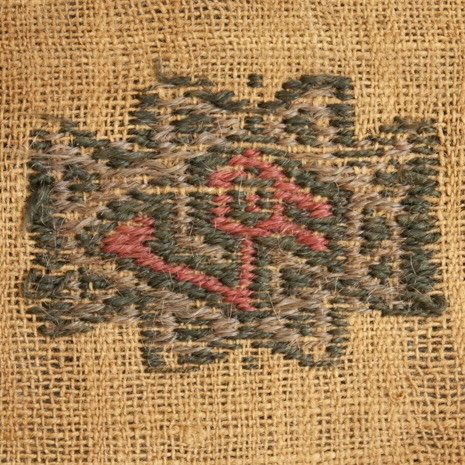
\includegraphics[width=5cm]{../images/VAM005_2.jpg}
		\caption{Détail du textile Nazca brodé de l'Intermédiaire Ancien. \\ Référence dans la base de données : VAM005.}
		\label{fig:VAM005_2}
	\end{center}
    \end{minipage}
    \hspace{5pt}
    \begin{minipage}[c]{.5\linewidth}
        \begin{center}
        		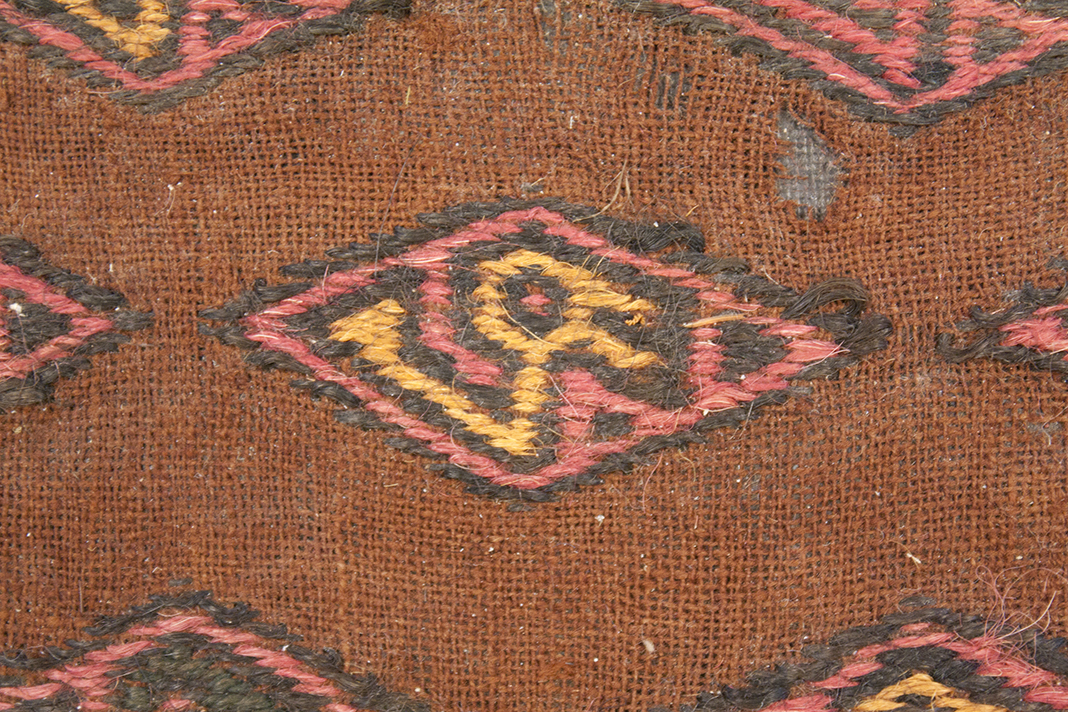
\includegraphics[height=5cm]{../images/BML048.jpg}
		\caption{Broderie Chancay, Intermédiaire Tardif.\\ Référence dans la base de données : BML048.}
		\label{fig:BML048}
	\end{center}
    \end{minipage}
\end{figure}

Un autre motif côtier présent dans ce \textit{cluster} illustre les phénomènes d'imitations ou de ré-interprétations. Un visage félin tissé en dominante trame est présent au sein de plusieurs textiles. Cet exemple est intéressant puisque contrairement aux motifs d'oiseaux, la base de données ne contient pas de tissage en dominante chaîne avec les mêmes motifs, à la même période et avec le même lieu de production. Pourtant, les motifs détiennent les traits caractéristiques d'un tissage à dominante chaîne, notamment la forme des yeux, de la bouche, les diagonales et la répartition régulière de points de couleurs différentes sur l'ensemble du textile. Il pourrait donc s'agir d'une ré-interprération en trame d'un motif, ou du moins d'un style, en dominante chaîne.

\begin{figure}[!h]
 \begin{minipage}[c]{.3\linewidth}
        \begin{center}
        		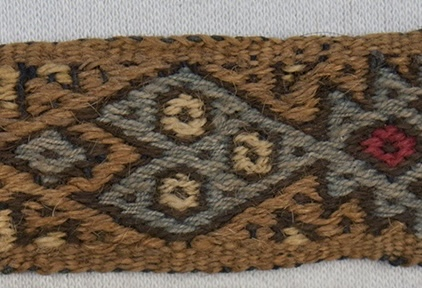
\includegraphics[width=5cm]{../images/BML072.jpg}
		\label{fig:BML072}
	\end{center}
    \end{minipage}
     \begin{minipage}[c]{.3\linewidth}
        \begin{center}
        		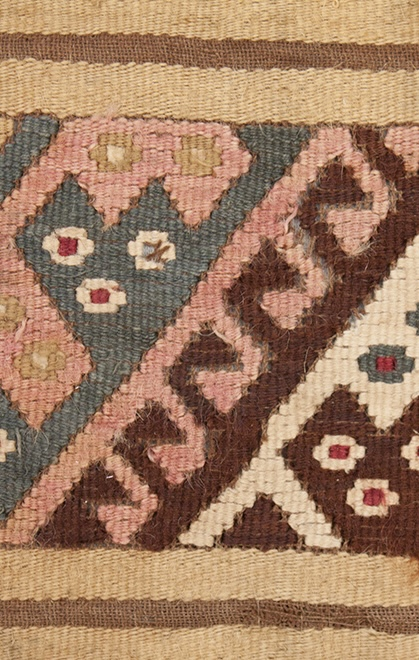
\includegraphics[width=4cm]{../images/BML045.jpg}
		\label{fig:BML045}
	\end{center}
    \end{minipage}
    \begin{minipage}[c]{.3\linewidth}
        \begin{center}
        		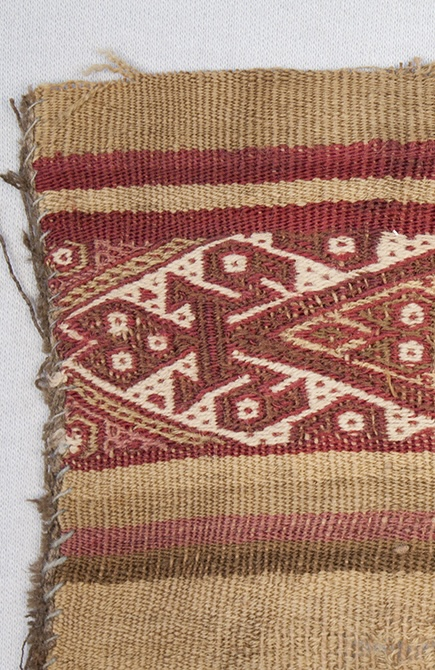
\includegraphics[width=4cm]{../images/BML083.jpg}
		\label{fig:BML083}
	\end{center}
    \end{minipage}
    \caption{Détails de tissages à dominante trame, Chancay, Intermédiaire Tardif. \\ Référence dans la base de données : BML072, BML045 et BML083.}
\end{figure}

Le \textit{cluster} 27, voisin du \textit{cluster} 7 contient également plusieurs visages félins. En outre, on y retrouve des textiles reprenant les motifs de serpents entremêlés que nous avons abordés dans le premier chapitre. Toutefois, ce cluster nous permet d'élargir la perspective que nous avons de ce motif car il apparaît à la fois comme imitation d'un tissage à dominante chaîne et comme ré-interprétation, plus tardive, de l'organisation des entités qui le composent.
\begin{figure}[!h]
    \begin{minipage}[c]{.5\linewidth}
            \begin{center}
                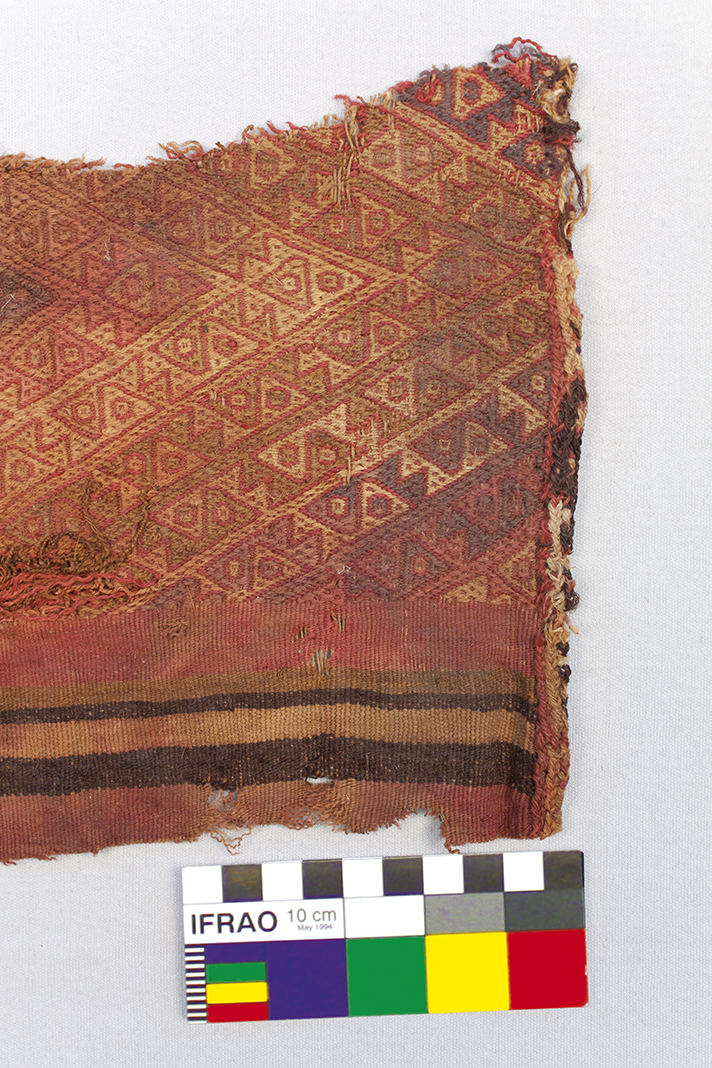
\includegraphics[height=8cm]{../images/BML069_avant.jpg}
                    \caption{Fragment de tapisserie avec trames \\ supplémentaires, Chancay, Intermédiaire Tardif. \\ Référence dans la base données : BML069.}
                \label{fig:BML069}   
            \end{center}
    \end{minipage}
    \hspace{5pt}
        \begin{minipage}[c]{.5\linewidth}
        \begin{center}
        		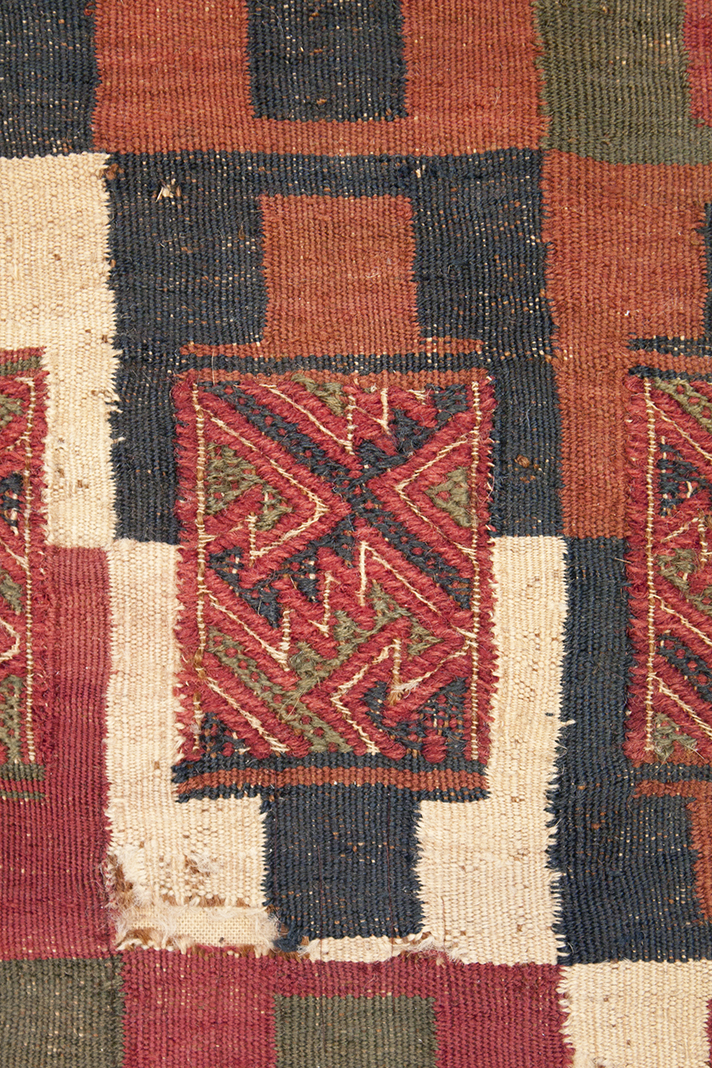
\includegraphics[height=8cm]{../images/BML094_detail.jpg}
		 \caption{Détail d'une tapisserie en style inca provincial (côte sud du Pérou), Horizon Tardif.\\ Référence dans la base données : BML094.}
		 \label{fig:BML094}
	\end{center}
    \end{minipage}
\end{figure}
\noindent La frontière entre ces deux \textit{clusters} est très poreuse puisque le cas de serpents entremêlés étudié au chapitre 1 (voir \ref{fig:BML044_avant}) se trouve dans le \textit{cluster} 7 alors que le reste des motifs de serpents se trouve dans le \textit{cluster} 27. Au vue de ses caractéristiques, ce motif semble prendre son origine d'un textile dominante chaîne, ré-interprété en trame. Mais il s'est diffusé sur la côte et peu à peu il semble avoir perdu les traits caractéristiques qui le rattachaient à sa technique initiale. En effet, dans sa ré-interprétation en trames supplémentaires dans une tapisserie inca, les points alternés ont disparu, ne restent que les diagonales et l'organisation des éléments triangulaires. On obtient ainsi une amorce de généalogie de ce motif que l'on observe à travers plusieurs civilisations, sur près de 500 ans.\\

La classification non-supervisée fournit une partition intéressante des textiles. Bien que certains \textit{clusters} soient très dépendants de la composition initiale des photographie, notamment du fond, les \textit{clusters} composés de détails de textiles fournissent des indices sur les imitations entre civilisations. La distinction entre la côte et les hautes-terres reste forte, avec des cas d'imitations. Toutefois, les \textit{clusters} qui se trouvent entre les \textit{clusters} \og haute-terre \fg \:et les \textit{clusters} \og côtiers \fg \:ne déterminent pas de traits communs entre les deux zones géographiques (\textit{clusters} 1 et 17), bien qu'on y trouve des pièces au croisement des hautes-terres et de la côte comme la tunique Nazca-Huari aux motifs de serpents entremêlés présentée dans le second chapitre (\ref{fig:VAM012}). Ils sont trop grands pour y trouver des éléments clairs de compréhension des échanges et des imitations textiles dans les Andes. Néanmoins, la répartition des textiles confirme la circulation côtière que nous avons observée à partir des informations géographiques présentes dans la base de données. Les échanges relevés dans le chapitre précédent (voir \ref{fig:distance_map}) sont confirmés par la proximité iconographique de certaines pièces. \\

Le recours à des outils d'intelligence artificielle nous permet de répondre à certaines de nos interrogations initiales. Les méthodes contemporaines de classification supervisée semblent adéquates à la détection d'armures textiles andines, renseignement majeur pour le traitement de grand corpus de textiles comme c'est le cas pour les Andes. Outre la détection des armures textiles, les outils de \textit{computer vision} nous permettent également de confirmer certaines hypothèses de circulation des textiles. La classification non-supervisée des textiles illustre la grande variété des textiles andins, et souligne les similarités entre civilisations côtières, notamment iconographiques. Malgré le peu de textiles coloniaux présents dans la base de données et leur simplicité, la classification non-supervisée tend à nous indiquer une rupture des textiles coloniaux par rapport aux textiles archéologiques, mais souligne également la continuité entre les \textit{mantas} coloniales et les \textit{mantas} républicaines.
